\documentclass[a4paper,11pt]{book}
\usepackage[utf8]{inputenc}
\usepackage[spanish]{babel}
\usepackage{graphicx}
\usepackage{listings}
\usepackage{cite}
\usepackage{url}

\decimalpoint
\usepackage{dcolumn}

\usepackage{colortbl,longtable}
\usepackage[stable]{footmisc}

\usepackage{fancyhdr}
\pagestyle{fancy}
\fancyhf{}
\fancyhead[LO]{\leftmark} % En las páginas impares, parte izquierda del encabezado, aparecerá el nombre de capítulo
\fancyhead[RE]{\rightmark} % En las páginas pares, parte derecha del encabezado, aparecerá el nombre de sección
\fancyhead[RO,LE]{\thepage} % Números de página en las esquinas de los encabezados
\renewcommand{\chaptermark}[1]{\markboth{\textbf{\thechapter. #1}}{}} % Formato para el capítulo: N. Nombre
\renewcommand{\sectionmark}[1]{\markright{\textbf{\thesection. #1}}} % Formato para la sección: N.M. Nombre

\renewcommand{\headrulewidth}{0.6pt} % Ancho de la línea horizontal bajo el encabezado
\renewcommand{\footrulewidth}{0.6pt} % Ancho de la línea horizontal sobre el pie (que en este ejemplo está vacío)
\setlength{\headheight}{1.5\headheight} % Aumenta la altura del encabezado en una vez y media


%\RequirePackage{verbatim}
%\usepackage{fancyhdr}
%\usepackage{graphicx}
%\usepackage{afterpage}
%\usepackage{longtable}
%\usepackage[pdfborder={000}]{hyperref} %referencia


% ********************************************************************
% Re-usable information
% ********************************************************************
\newcommand{\myTitle}{Visualización de datos en procesamiento masivo de Big Data\xspace}
\newcommand{\myDegree}{Grado en Ingeniería Informáticaxspace}
\newcommand{\myName}{Adrián Medina González (alumno)\xspace}
\newcommand{\myProf}{José Manuel Benítez Sánchez (tutor1)\xspace}
\newcommand{\myOtherProf}{Manuel Jesús Parra Royón (tutor2)\xspace}
\newcommand{\myFaculty}{Escuela Técnica Superior de Ingenierías Informática y de
	Telecomunicación\xspace}
\newcommand{\myFacultyShort}{E.T.S. de Ingenierías Informática y de
	Telecomunicación\xspace}
\newcommand{\myDepartment}{Departamento de Ciencias de la Computación e Inteligencia Artificial\xspace}
\newcommand{\myDepartmentShort}{Departamento de DECSAI\xspace}
\newcommand{\myUni}{\protect{Universidad de Granada}\xspace}
\newcommand{\myLocation}{Granada\xspace}
\newcommand{\myTime}{\today\xspace}
\newcommand{\myVersion}{Version 0.1\xspace}

\usepackage{pdfpages}

%Para conseguir que en las páginas en blanco no ponga cabecerass
\makeatletter
\def\clearpage{%
	\ifvmode
	\ifnum \@dbltopnum =\m@ne
	\ifdim \pagetotal <\topskip
	\hbox{}
	\fi
	\fi
	\fi
	\newpage
	\thispagestyle{empty}
	\write\m@ne{}
	\vbox{}
	\penalty -\@Mi
}
\makeatother

%\setlength{\parindent}{1.5em}
%\setlength{\parskip}{5pt}

%\setlength{\parskip}{1em} 
%\renewcommand{\baselinestretch}{2.0}

\setlength{\parskip}{15pt plus 1pt minus 2pt}

\begin{document}

\begin{titlepage}

	\newlength{\centeroffset}
	\setlength{\centeroffset}{-0.5\oddsidemargin}
	\addtolength{\centeroffset}{0.5\evensidemargin}
	\thispagestyle{empty}
	
	\noindent\hspace*{\centeroffset}\begin{minipage}{\textwidth}
		
		\centering
		
\includegraphics[width=0.9\textwidth]{imagenes/logo_ugr.jpg}\\[1.4cm]
		
		\textsc{ \Large TRABAJO FIN DE GRADO\\[0.2cm]}
		\textsc{GRADO EN INGENIERÍA INFORMÁTICA}\\[1cm]
		% Upper part of the page
		% 
		% Title
		{\Huge\bfseries Visualización de datos\\
		}
		\noindent\rule[-1ex]{\textwidth}{3pt}\\[3.5ex]
		{\large\bfseries Visualización de datos en procesamiento masivo de Big Data}
	\end{minipage}
	
	\vspace{2.5cm}
	\noindent\hspace*{\centeroffset}\begin{minipage}{\textwidth}
		\centering
		
		\textbf{Autor}\\ {Adrián Medina González}\\[2.5ex]
		\textbf{Directores}\\
		{José Manuel Benítez Sánchez\\
			Manuel Jesús Parra Royón}\\[2cm]
		
\includegraphics[width=0.3\textwidth]{imagenes/etsiit_logo.png}\\[0.1cm]
		\textsc{Escuela Técnica Superior de Ingenierías Informática y de Telecomunicación}\\
		\textsc{---}\\
		Granada, Septiembre de 2017
	\end{minipage}
	%\addtolength{\textwidth}{\centeroffset}
	%\vspace{\stretch{2}}
\end{titlepage}

\chapter*{}
\thispagestyle{empty}

\noindent\rule[-1ex]{\textwidth}{2pt}\\[4.5ex]

Yo, \textbf{Adrián Medina González}, alumno de la titulación de la \textbf{Escuela Técnica Superior
de Ingenierías Informática y de Telecomunicación de la Universidad de Granada}, con DNI 76627532L, autorizo la
ubicación de la siguiente copia de mi Trabajo Fin de Grado en la biblioteca del centro para que pueda ser
consultada por las personas que lo deseen.

\vspace{6cm}

\noindent Fdo: Adrián Medina González

\vspace{2cm}

\begin{flushright}
Granada, Septiembre de 2017 .
\end{flushright}


\chapter*{}
%\thispagestyle{empty}

\noindent\rule[-1ex]{\textwidth}{2pt}\\[4.5ex]

D. \textbf{José Manuel Benítez Sánchez}, Profesor del Departamento Ciencias de la Computación e Inteligencia Artificial de la Universidad de Granada.
%\vspace{0.5cm}

D. \textbf{Manuel Jesús Parra Royón}, Profesor del Departamento Ciencias de la Computación e Inteligencia Artificial de la Universidad de Granada.
%\vspace{0.5cm}

\textbf{Informan:}
%\vspace{0.5cm}

Que el presente trabajo, titulado \textit{\textbf{Visualización de datos en procesamiento masivo de Big Data}},
ha sido realizado bajo su supervisión por \textbf{Adrián Medina González}, y autorizamos la defensa de dicho trabajo ante el tribunal
que corresponda.

%\vspace{0.5cm}

Y para que conste, expiden y firman el presente informe en Granada, Septiembre de 2017 .

%\vspace{1cm}

\textbf{Los directores:}

\vspace{5cm}

\noindent \textbf{José Manuel Benítez Sánchez \ \ \ \ \ Manuel Jesús Parra Royón}

\chapter*{Agradecimientos}
\thispagestyle{empty}

\vspace{1cm}


Quiero agradecer a los tutores José Manuel Benítez Sánchez y Manuel Jesús Parra Royón por el tiempo y el esfuerzo invertidos en la realización de este proyecto. 

También agradezco a la ETSIIT por permitirme trabajar con parte de los servidores para poder ejecutar la aplicación. 

Por último, agradezco toda la paciencia y el apoyo mostrados durante este tiempo a mi familia, especialmente a Verónica que ha convivido diariamente con los buenos y malos momentos durante la realización del proyecto. 



\tableofcontents


\chapter{Introducción}

\section{Motivación}

En todo el mundo se recopila y almacena una gran cantidad de información, a través de las nuevas tecnologías, nuevos productos, aplicaciones, etc, la conectividad entre personas de cualquier parte del planeta, o incluso, la comunicación entre dispositivos. Todo ello, genera una cantidad de información de dimensiones que rondan los \textit{petabytes} o los \textit{exabytes}, teniendo en cuenta además, que la procedencia de los datos es muy variable y, por tanto, la estructura en la que se recibe. 

Poder controlar la información y la posibilidad de utilizarla en su beneficio, es el pilar principal de todas las grandes y medianas empresas del mundo. Sin embargo, a raíz de este aumento de los datos, las herramientas clásicas para analizarlos, se han quedado inutilizadas al no tener la capacidad de manejarlos. Por tanto, existe la necesidad de diseñar nuevas herramientas que sean capaces de abordar el conocido problema del \textit{BigData}. 

Una vez conseguido manejar y controlar de manera eficiente la información, hay que considerar que los datos en sí, pueden no aclarar su significado realmente. Las representaciones gráficas de los mismos, ayudan a entender su comportamiento de una forma sencilla, incluso para aquellos que no tengan el suficiente conocimiento de análisis. Algunos de los gráficos clásicos como el histograma, el diagrama de cajas o bigotes, o el diagrama de puntos, son básicos en las herramientas de exploración de datos. El límite está, como se ha explicado anteriormente, que son herramientas que no están preparadas para procesar un gran volumen de datos. Por ello, es necesario el diseño de una herramienta que sea capaz de extrapolar la visualización de los datos para una enorme cantidad de datos.

\section{Objetivos}
El objetivo principal de este proyecto es crear una biblioteca capaz de generar representaciones gráficas a partir de grandes conjuntos de datos, conocidos como 'Big Data'. Para conseguirlo, se ha desglosado en varios objetivos distintos:
\begin{itemize}
	\item Crear una biblioteca que, dados unos datos de entrada de tipo 'Big Data', sea capaz de procesar tal cantidad de información, para obtener como resultado variables o datos que necesita cada uno de los gráficos para su representación, como pueden ser valores máximos o mínimos del conjunto de datos, cuartiles, medias, agrupaciones de variables discretas, etc. La complejidad de este objetivo es obtener estos valores a partir de datos que superan fácilmente el millón de registros.
	\item Dotar a la herramienta de una API RESTful, que permite obtener información de cada una de las funciones que se han implementado, con la posibilidad de ejecutarlas de forma individual.
	\item Construir una interfaz web que permita el acceso y la utilización de la herramienta de manera sencilla, eficaz y accesible desde cualquier plataforma o dispositivo.
\end{itemize}

\section{Estructura del documento}

La estructura que sigue este documento se basa en explicar por apartados cada uno de los pasos y procedimientos que sigue la API diseñada. 

En el apartado número 2 del índice se habla sobre la situación en la que se encuentra la computación en Big Data ahora mismo, se explican las herramientas principales para construir la API, como \textit{Hadoop} o \textit{Spark}, y también se habla sobre la visualización de los datos aplicada a la gran cantidad de datos y el proceso que conlleva para obtener un gráfico sencillo de interpretar a partir de toda esa información. 

En el siguiente apartado, se desarrollan la planificación que se han seguido para crear la API, la metodología y los distintos lenguajes de programación que se han implementado.

En los apartados 4 y 5 del documento, se habla de las especificaciones técnicas de la aplicación, requisitos funcionales y no funcionales, y sobre el diseño del sistema, explicando su arquitectura, la conexión entre los distintos módulos, etc.

En el sexto módulo, se explican cada uno de los métodos de visualización que se han empleado, el procedimiento en cada uno de ellos para resumir la información entrante, y obteniendo un resultado que realmente refleje el comportamiento de los datos.

Por último, hay un apartado de conclusiones donde se explica cuales de los objetivos principales se han conseguido lograr o la finalidad de la API.

\chapter{Computación en BigData y Visualización de Datos}

En este capítulo se van ha explicar algunos temas más generales como el Big Data y la implicación que tiene en la sociedad, las herramientas utilizadas principalmente para gestionar tanta información guardada, y el proceso de adaptar las técnicas clásicas para generar diagramas al nuevo enfoque sobre Big Data.

\section{BigData}

En la actualidad, las grandes empresas del mundo gestionan grandes cantidades de información. Cuando se define que cantidad de datos va relacionada con \textit{BigData}, se habla de terabytes, petabytes, o incluso, exabytes. Aparte del gran volumen de información, también es importante tener en cuenta la variedad de los datos, su estructura y procedencia, por ejemplo, redes sociales, telefonía móvil, geolocalización, etc. No solo se genera información entre personas y ordenadores, sino que la comunicación entre distintos dispositivos, para mantener todas las herramientas interconectadas, genera una inmensa cantidad de datos de gran valor \cite{BigDataIntro}. 

Por eso, surge la necesidad de controlar y gestionar toda esta información tan diversa a través de nuevas técnicas, ya que los procesos y herramientas tradicionales son incapaces de procesar y analizar esta gran cantidad de información. Cuando el simple hecho de aumentar la capacidad hardware de los servidores de almacenamiento es insuficiente, es necesario utilizar algoritmos capaces de realizar esta tarea de manera rápida, sencilla y precisa. Por eso, uno de los principales paradigmas de programación de la actualidad, capaz de procesas la información \textit{BigData}, es el conocido MapReduce. MapReduce es el algoritmo capaz de procesar esas grandes cantidades de datos, y las herramientas utilizadas en este proyecto que implementan dicho algoritmo han sido Hadoop y Spark, de las que se va a tratar con mayor profundidad en los apartados siguientes.

Además del algoritmo MapReduce, la visualización de los datos también es un enfoque importante para ayudar a Big Data a obtener una visión completa de los datos y descubrir sus valores. Tanto el análisis como la visualización de \textit{BigData} deben integrarse perfectamente para su correcto funcionamiento en distintas aplicaciones. La visualización representa datos de una forma sistemática que permite a las grandes empresas mezclar fuentes de datos dispares para crear vistas analíticas personalizadas \cite{BigDataVisualization}. La analítica visual en \textit{BigData} se enfrenta a una serie de retos que vienen definidos por la “Regla de las 4 V’s”. Los retos de las 4 V’s serían los siguientes \cite{OverviewBigDataVis}: 

\begin{itemize}
	\item Volumen: Los métodos se desarrollan para trabajar con grandes volúmenes de datos y permiten derivar el significado de grandes volúmenes de datos.
	\item Variedad: Los métodos se desarrollan para combinar tantas fuentes de datos como sea necesario (estructurados y no estructurados).
	\item Velocidad: Con los métodos de visualización, las empresas pueden reemplazar los procesos batch por procesamiento en tiempo real.
	\item Valor: los métodos no sólo permiten a los usuarios crear infogramas llamativos, sino también aumentar el valor de negocio mediante la obtención de conocimientos a partir de \textit{BigData}.
\end{itemize}

\section{MapReduce}

El paradigma MapReduce es un modelo de programación enfocado en resolver los problemas de computación de grandes cantidades de datos, de manera paralela y distribuida. Este estilo de programación se creó inspirado en dos funciones de programación funcional: Map y Reduce. El objetivo de MapReduce es resolver problemas con conjunto de datos muy grandes, y por eso, se centra en la paralelización de los cálculos. 

\begin{figure}
	\centering
	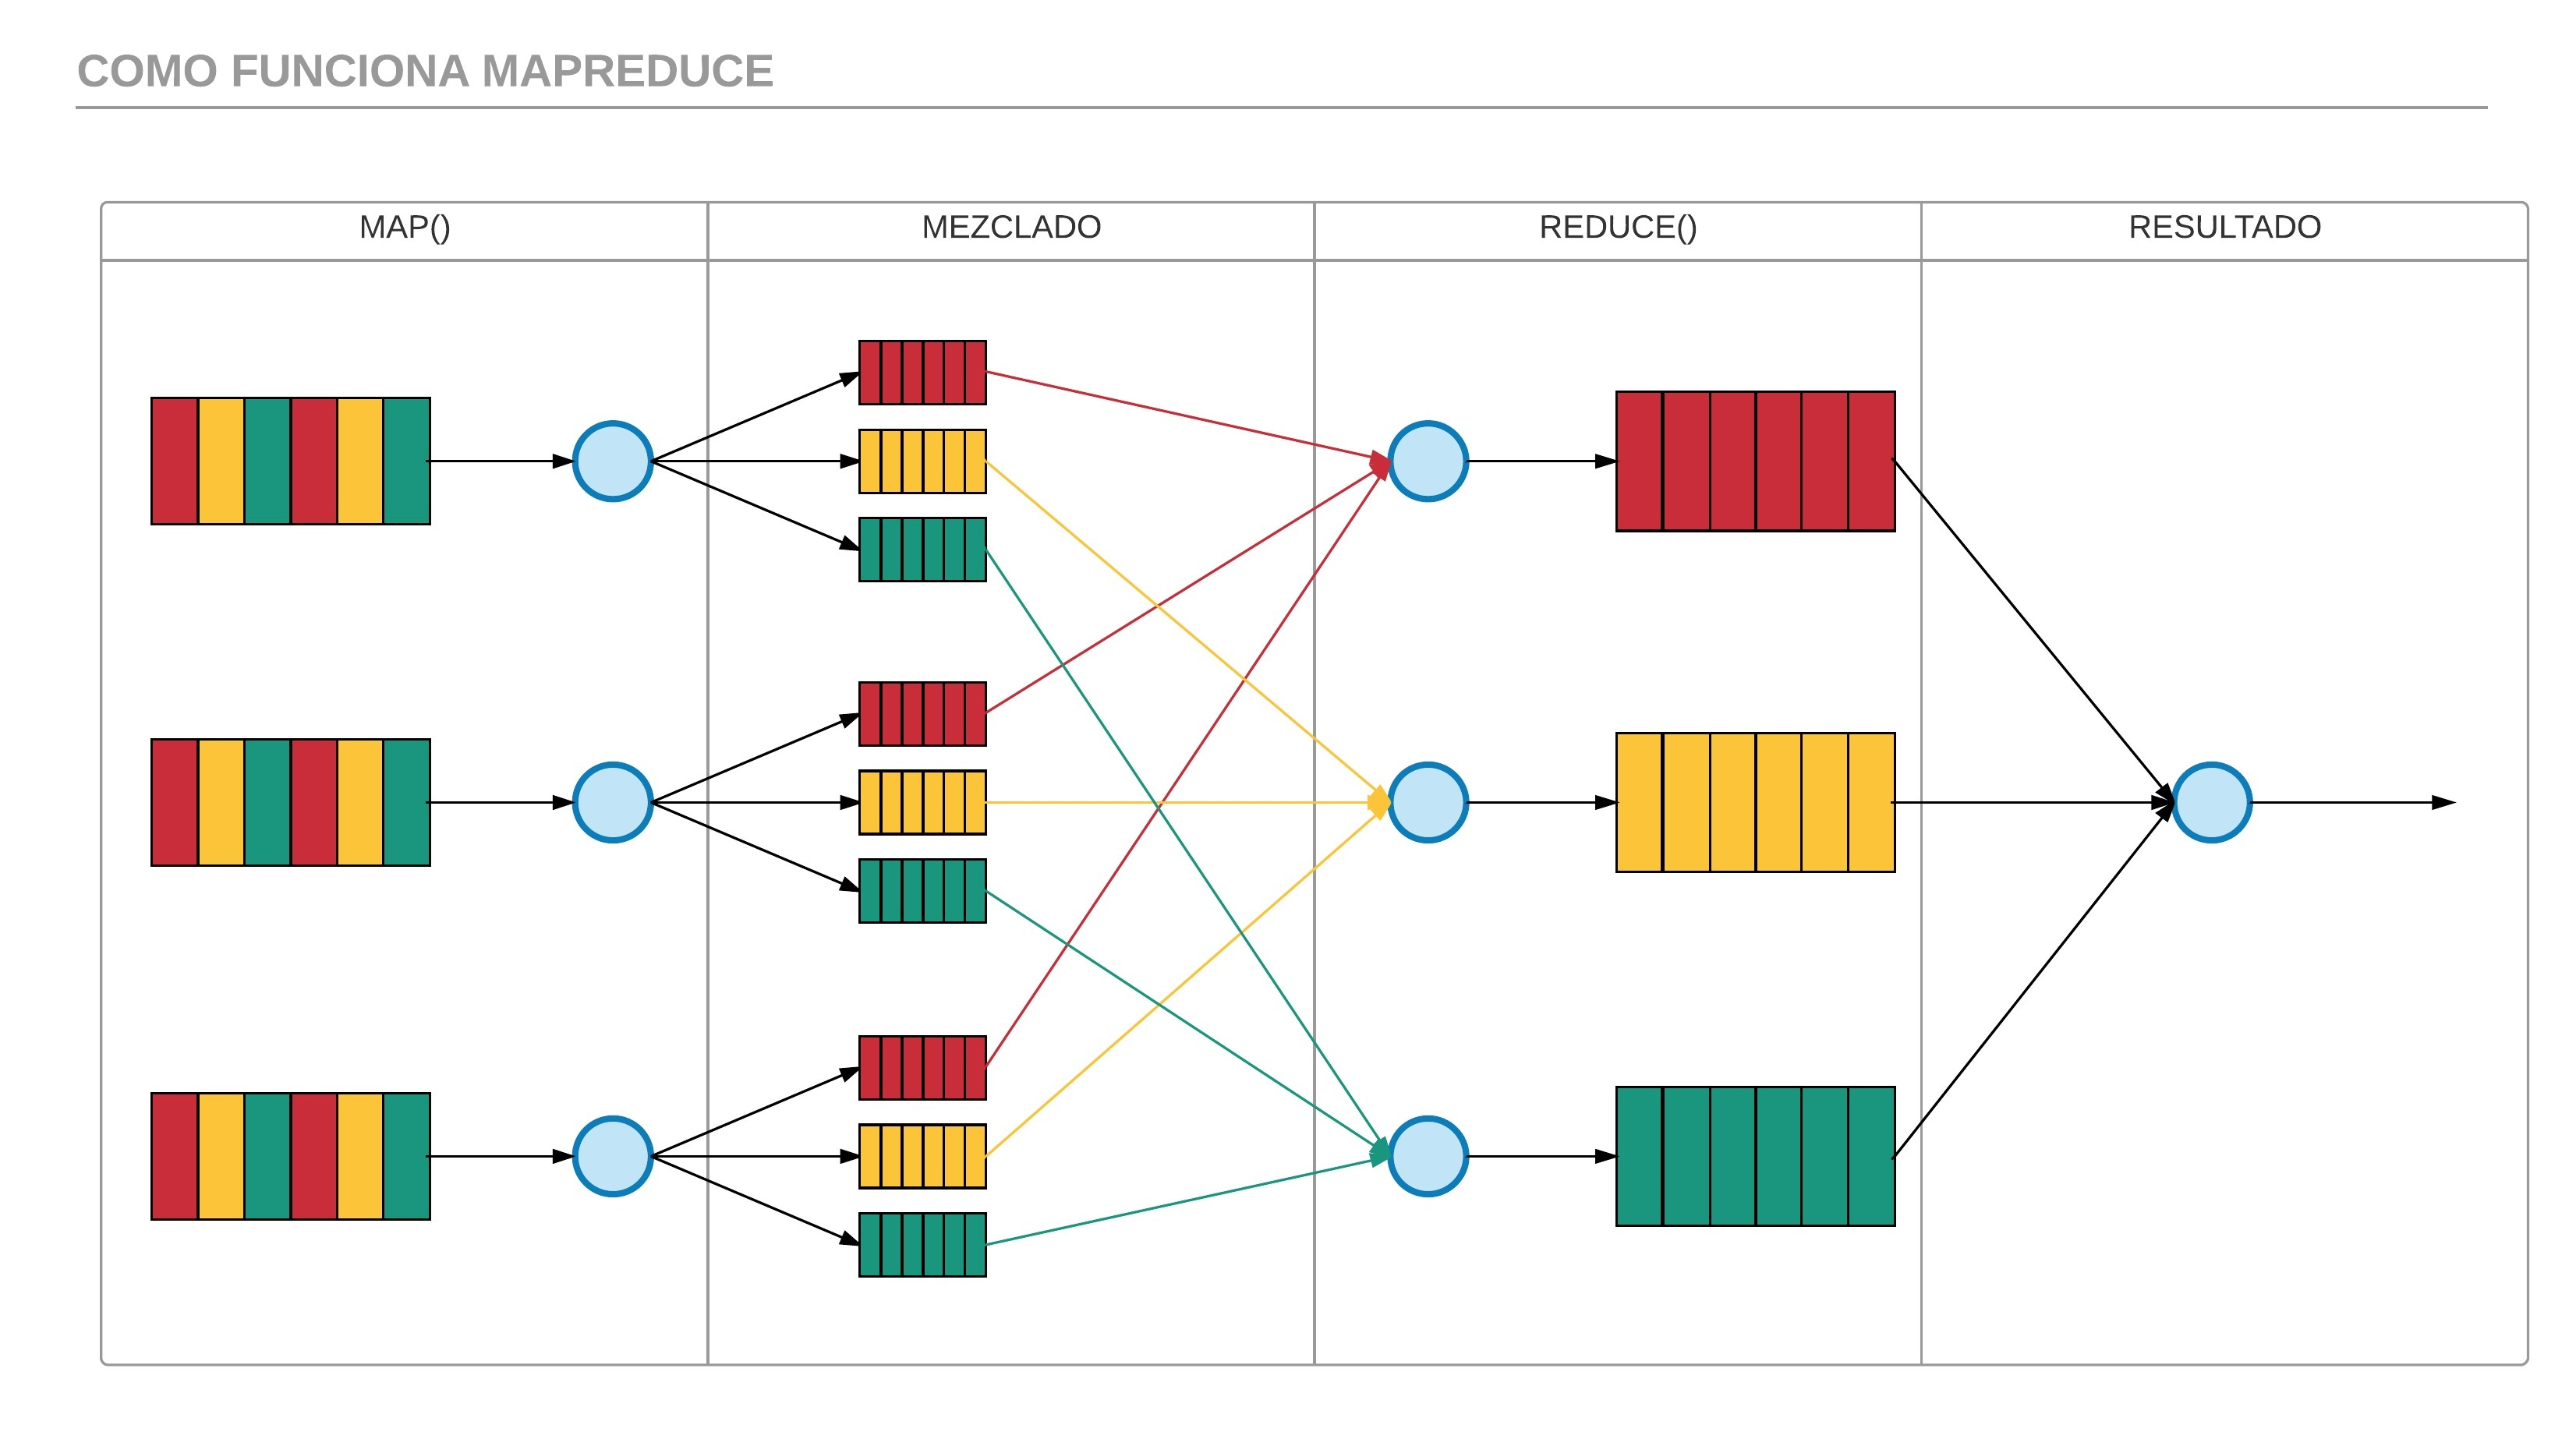
\includegraphics[width=1\linewidth]{imagenes/Como_funciona_MapReduce}
	\caption{Funcionamiento de MapReduce}
	\label{fig:comofuncionamapreduce}
\end{figure}

Se puede explicar el funcionamiento de MapReduce como una división del cálculo en distintas fases, como se aprecia gráficamente en la figura \ref{fig:comofuncionamapreduce}.
Primero una fase de mapeo o transformación de datos, la cual se encarga de aplicar una función de cómputo sobre los mismos, manteniéndose dentro de la misma fase el resultado del procesamiento. Este resultado no se almacena en el momento de ejecutar la función, sino que se acumulan todas las transformaciones hasta la segunda fase. En esta segunda fase se realizan las llamadas acciones o funciones de reducción, que se encargan de calcular un resumen de los datos, como puede ser una sumatoria, como se muestra en la figura \ref{fig:flujodedatosenmapreduce}.

\begin{figure}
	\centering
	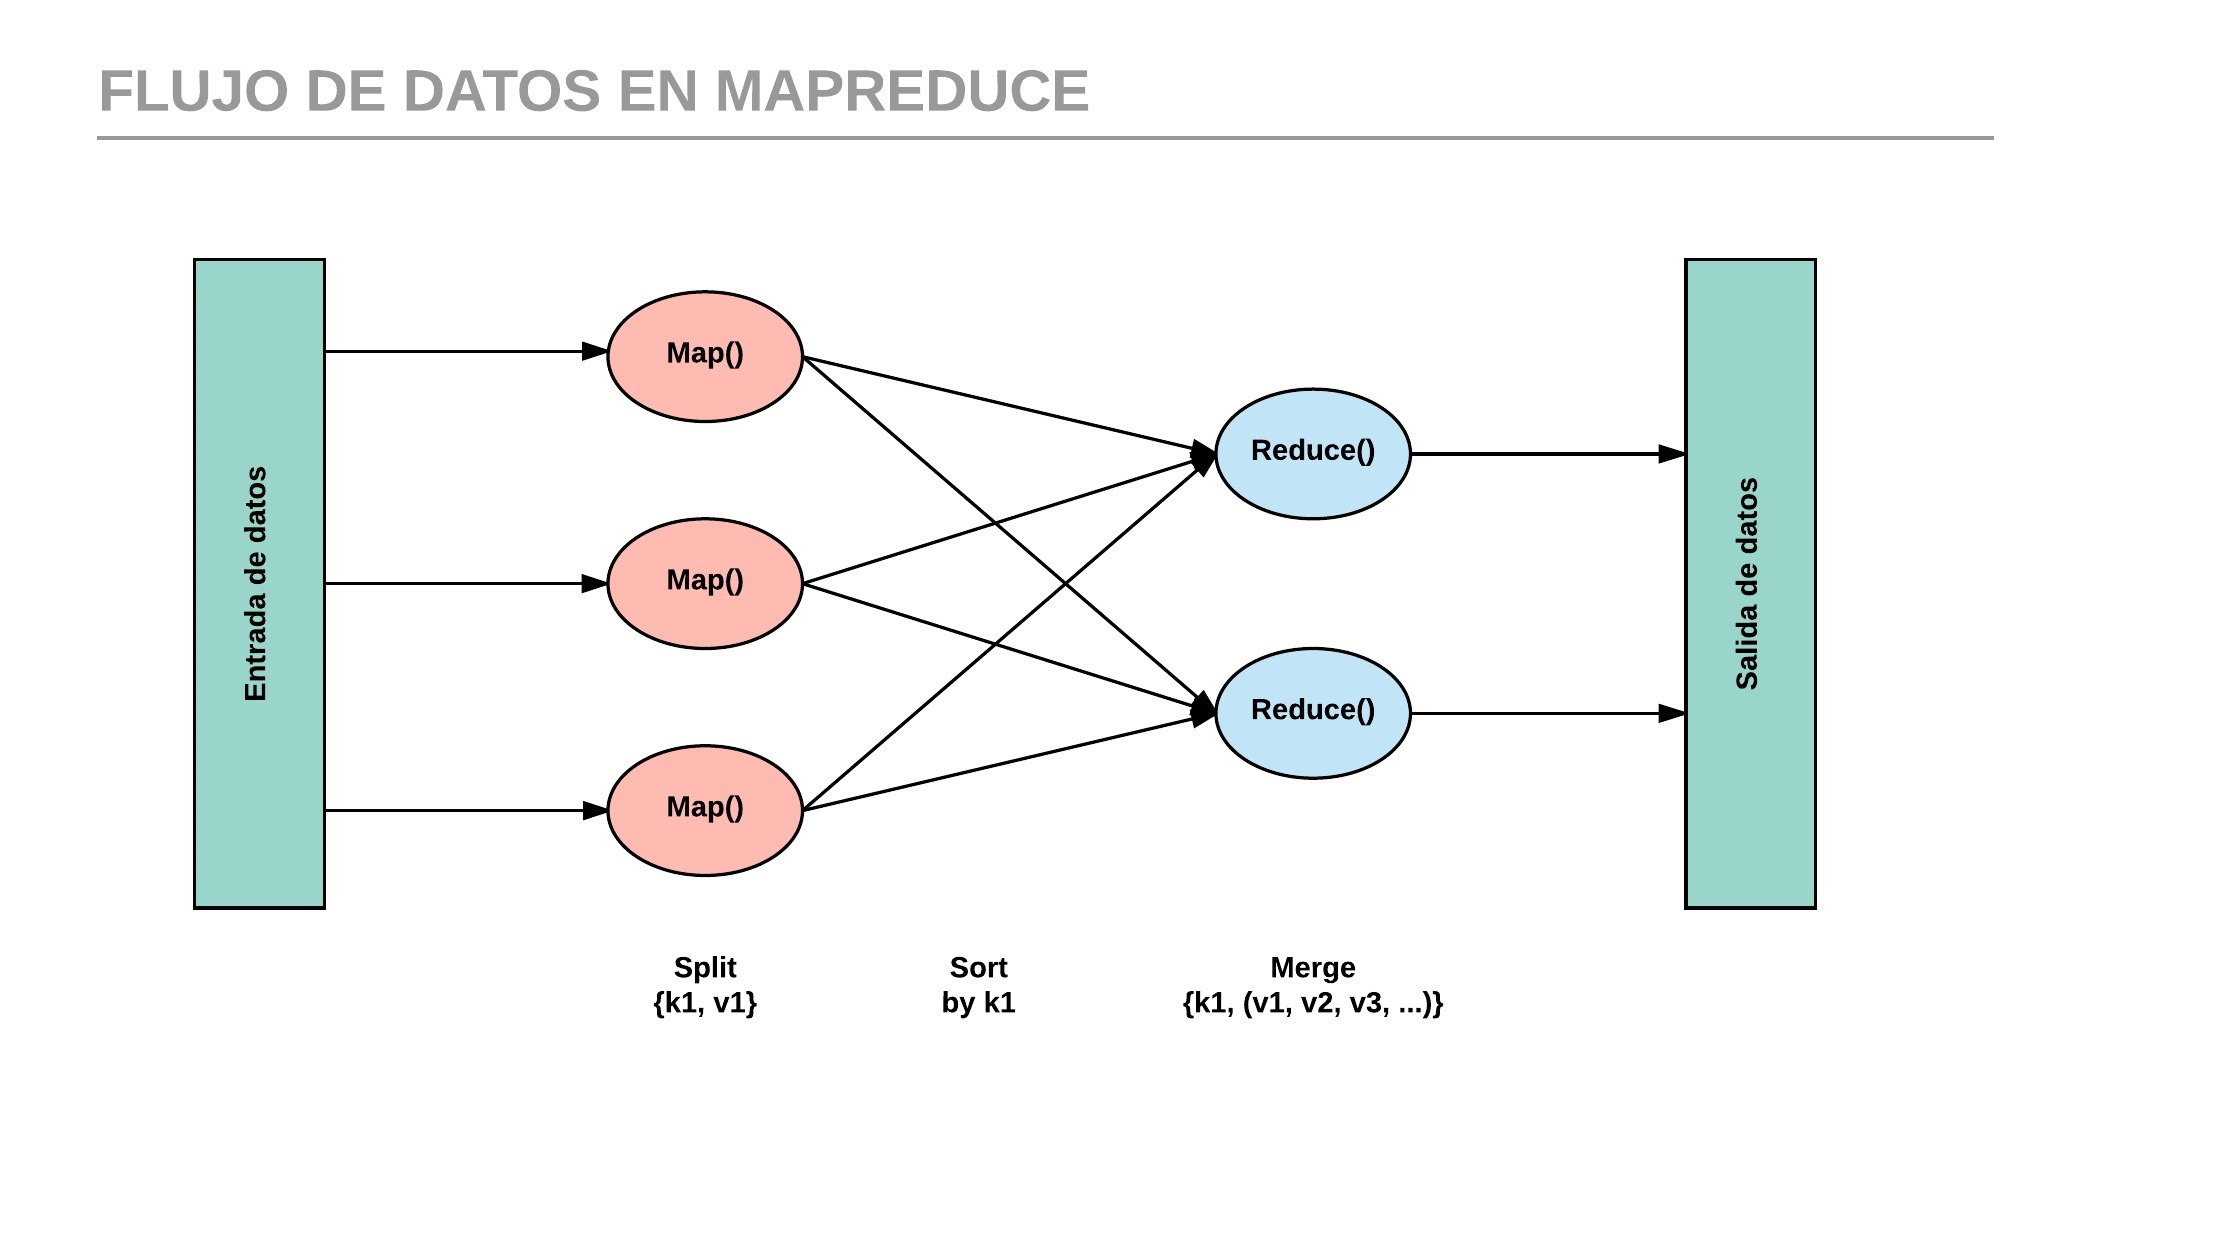
\includegraphics[width=1\linewidth]{imagenes/Flujo_de_datos_en_MapReduce}
	\caption{Flujo de datos en MapReduce}
	\label{fig:flujodedatosenmapreduce}
\end{figure}

En cada una de las fases se elige una o varias funciones correspondientes de la misma. Los datos se adaptan a una estructura ‘key-value’ para poder subdividir una tarea entre los distintos recursos disponibles \cite{MRHadoopLibro}. 

\section{Hadoop}
\begin{minipage}{\textwidth}
	\centering
	
\includegraphics[width=0.4\textwidth]{imagenes/hadoop_logo.png}\\[0.1cm]
\end{minipage}

\textbf{Apache Hadoop} \cite{HadoopInicial} es un entorno de trabajo Open-Source que ofrece computación escalable y distribuida, sobre grandes conjuntos de datos. Hadoop permite la escalabilidad desde un servidor, hasta cientos de ellos, solamente ajustando unos pocos parámetros \cite{HadoopInicial}. Este framework ofrece una amplia gama de funcionalidad gracias a tres grandes cualidades que posee:
\begin{itemize}
	\item La escalabilidad, permitiendo guardar y distribuir enormes conjuntos de datos en cientos de servidores que funcionan en paralelo. 
	\item La flexibilidad que ofrece con respecto al tipo de datos que almacena, es una de las grandes ventajas del sistema, ya que no importa el tipo de fichero que se quiere guardar o la fuente de la que provienen. 
	\item Su tolerancia a fallos lo hace uno de los más robustos del mercado, ya que el propio sistema siempre mantiene copias de los datos en los distintos nodos de los clusters, permitiendo la posibilidad de recuperarse en caso de errores.	
\end{itemize}

La estructura de Hadoop está basada en cuatro grandes módulos, que se detallan a continuación:
\begin{itemize}
	\item Hadoop Common: Este módulo es la base de Hadoop. Proporciona los ficheros fuente del sistema, necesarios para su ejecución sobre los cluster. También proporciona la documentación necesaria para la instalación y ejecución.
	\item Hadoop Distributed File System (HDFS): Se trata de un sistema de archivos que permite acceder a los datos guardados en el servidor. Tiene un gran nivel de abstracción, lo que permite acceder a los archivos de datos de manera fácil, sin la necesidad de conocer la ubicación real, es decir, en que cluster se encuentran los datos. Es tal abstracción, que si los ficheros están fraccionados y ubicados en distintas localizaciones internamente, seguiría visualizándose como un único archivo y procesándose como tal.
	
	La estructura HDFS se divide en dos conceptos clave, un ‘Namenode’ y múltiples ‘Datanode’. Este concepto se basa en la estructura clásica maestro-esclavo, donde el Namenode sería la de maestro, cuya función es gestionar el espacio de nombres del sistema de archivos y controlar el acceso por parte de los clientes a los archivos. Los Datanodes, por el contrario, son la parte esclava de la estructura. Suele haber uno por cluster en el servidor donde se ejecuta HDFS. 
	La función de esta estructura es dividir los ficheros de datos en varios bloques, que se almacenan en los distintos Datanodes, replicando algunos de estos mismos bloques en varios Datanodes para ofrecer una tolerancia a fallos mayor. En el caso del Namenode, se encarga de dirigir que Datanode almacena cada parte del archivo, teniendo siempre constancia de cada una de la ubicación.
	
	Por parte del cliente, permite realizar operaciones como abrir, modificar, borrar archivos, etc, sin la necesidad de conocer la localización del mismo \cite{HDFSHadoopLibro}.  Se puede apreciar, de manera más gráfica, el sistema HDFS en la figura \ref{fig:hdfsestructura}.
	\item Hadoop YARN: Es un framework que permite gestionar los recursos disponibles para la instalación y ejecución de Hadoop. Se trata de una herramienta para gestionar los clusters disponibles, configurar el comportamiento de cada uno de ellos, y poder balancear la carga de trabajo de cada uno de ellos. Suele utilizarse una estructura Maestro-Esclavo en los sistemas Hadoop.
	\item Hadoop MapReduce: La base de Hadoop es el paradigma MapReduce, explicado anteriormente. Está orientado a resolver problemas con grandes conjuntos de datos, por lo que utiliza el sistema de archivos distribuido (HDFS).
\end{itemize}

\begin{figure}
	\centering
	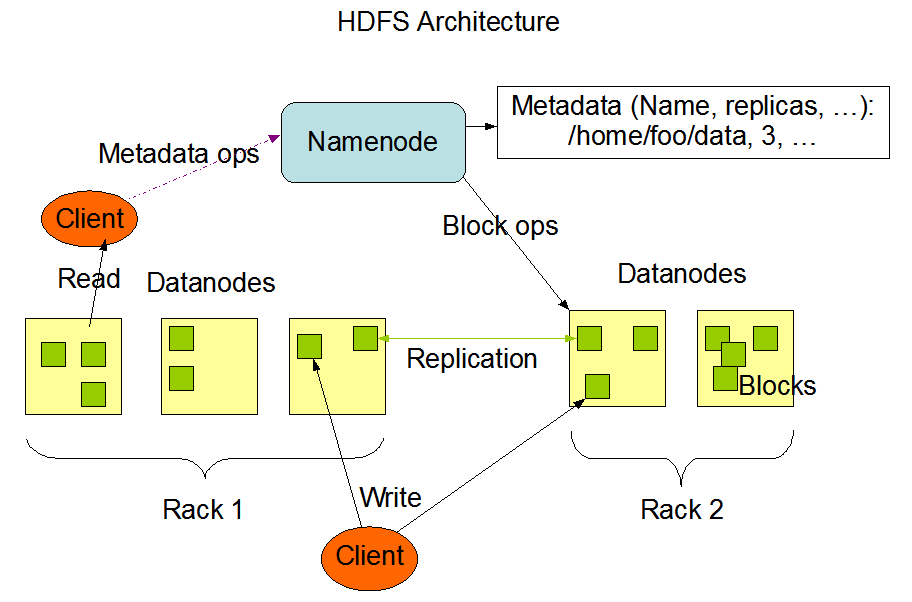
\includegraphics[width=1\linewidth]{imagenes/hdfs_estructura}
	\caption{Arquitectura del HDFS \cite{HadoopHDFS}}
	\label{fig:hdfsestructura}
\end{figure}

En la API, la idea de usar Hadoop es como almacenamiento y gestión de los ficheros de datos, gracias a las ventajas que ofrece para detectar y gestionar fallos. Otra de las grandes ventajas es su fácil y precisa conexión con la herramienta Apache Spark. Esta nueva herramienta, permite suprimir algunas de las carencias de Hadoop, como por ejemplo, tener una API sencilla con la que trabajar en lenguajes como Scala (su lenguaje nativo), Java, Python o SparkSQL. Otra de las debilidades de Hadoop es su rendimiento, ya que todos los datos están en disco, pero Spark cubre esta carencia pudiendo trabajar en memoria. Como resultado de esto, todos los cálculos se aceleran considerablemente, y hablando de grandes volúmenes de datos, es imprescindible la rapidez. 
En la siguiente sección, se explica con detalle la funcionalidad de Spark.

\section{Spark}

\begin{minipage}{\textwidth}
	\centering
	
\includegraphics[width=0.3\textwidth]{imagenes/spark_logo.png}\\[0.1cm]
\end{minipage}

\textbf{Apache Spark} \cite{SparkInicial} es un entorno de trabajo Open-Soruce diseñador para procesar grandes cantidades de datos de una manera sencilla, rápida y con grandes capacidades de analítica. En los últimos años, se ha alzado como un referente en la computación de Big Data, al solucionar algunas carencias que tiene Hadoop, y mejorar otros aspectos fundamentales. Principalmente, mejora el paradigma MapReduce haciéndolo más rápido y con procesamiento de datos en tiempo real, gracias al cómputo de los mismos en memoria \cite{SparkInicial}.

Una de las grandes ventajas de Spark es su soporte para compilar código en varios lenguajes, como Scala, Java, Python o R. Esto confiere a la herramienta una gran versatilidad cuando se trabaja con ella.

Las aplicaciones diseñadas en Spark se ejecutan como conjuntos independientes de procesos sobre un cluster. El encargado de coordinar estos procesos es el objeto SparkContext \cite{SparkClusterOverview}.

Para ejecutarse en un cluster, el objeto SparkContext se conecta a los gestores de cada uno de los clusters, como por ejemplo Spark Mesos o YARN. Estos son los encargados de asignar los recursos disponibles entre las aplicaciones. Una vez ejecutado, Spark obtiene el control de los procesos ejecutores, encargados de gestionar los cálculos y el almacenamiento de datos de la aplicación. Por último, Spark envía el código de la aplicación (contenido en archivos JAR o Python controlados por SparkContext) a los ejecutores, para que estos lo ejecuten.

Cada una de las aplicaciones que se ejecutan en Spark, tienen su propio proceso ejecutor. Esto quiere decir, que son independientes entre sí, tanto en el lado de la programación como en el ejecutor. Están completamente aisladas, por lo que cada una tiene sus propios recursos del sistema. Sin embargo, esto significa también que no se comparten los datos entre las distintas instancias de los objetos SparkContext, a menos que estén localizados en un sistema de almacenamiento externo a Spark. 

\begin{figure}
	\centering
	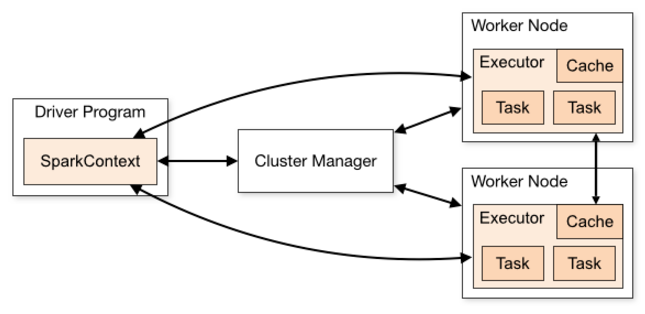
\includegraphics[width=1\linewidth]{imagenes/spark_estructura}
	\caption{Estructura del funcionamiento interno de Spark \cite{SparkClusterOverview}}
	\label{fig:sparkestructura}
\end{figure}

En un nivel de abstracción alto, cada una de las aplicaciones de Spark consiste en un programa controlador, que ejecuta el código diseñado por el usuario, encargándose el propio Spark de dividir y ejecutar las funciones paralelas dentro del mismo código sobre el cluster.
La principal abstracción que proporciona Spark es el conocido RDD (Resilient Distributed Dataset) \cite{SparkRDD}. RDD es una colección de elementos divididos a través de los nodos del cluster que pueden funcionar en paralelo. Una de las maneras de crear un RDD es con un archivo dentro del sistema de archivos de Hadoop (HDFS), por ejemplo. La recuperación automática que ofrece un RDD ante fallos en los nodos, es una de las grandes características que tienen. 

Otra característica de Spark son sus variables compartidas entre las funciones que se ejecutan en paralelo. Cuando se ejecutan estas funciones, Spark envía una copia de todas las variables utilizadas en la función a cada una de las tareas, ya que a veces una variable necesita ser compartida entre distintas tareas, o entre las tareas y el programa administrador. Hay dos tipos de variables compartidas distintas:
\begin{itemize}
	\item Variables de difusión: Se utilizan para almacenar en caché un valor compartido en todos los nodos.
	\item Acumuladores: Se utilizan para guardar resultados de operaciones de tipo \textit{reduce}.
\end{itemize}

\begin{figure}
	\centering
	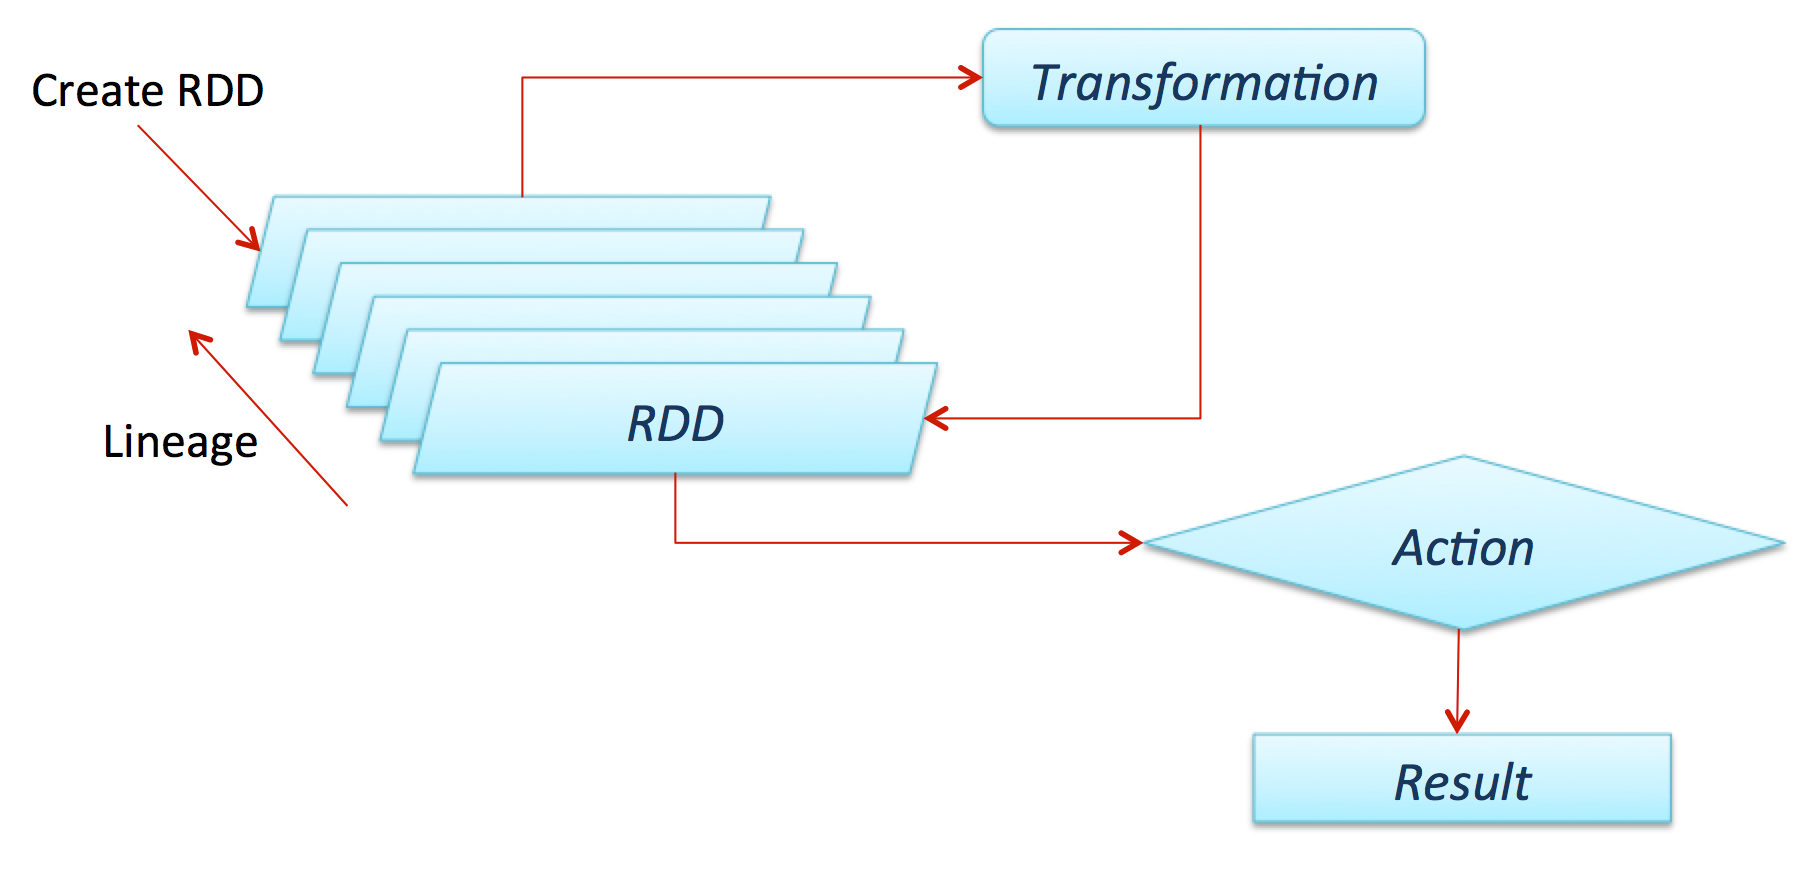
\includegraphics[width=1\linewidth]{imagenes/spark_rdd}
	\caption{Funcionamiento de un RDD \cite{SparkRDDFuncionamiento}}
	\label{fig:sparkrdd}
\end{figure}

La combinación de Hadoop y Spark, crea una potente herramienta para el cómputo y análisis de grandes cantidades de datos. En la API, la principal función de Spark es de conexión con los ficheros almacenados en cluster con HDFS, la aplicación de técnicas de reducción y agrupación de los mismos, y el cómputo de los datos para obtener un resultado que pueda ser interpretado y representado gráficamente.
Además, permite la ejecución paralela de varios procesos, dándole una potencialidad mayor a la API.

\section{MongoDB}
\begin{minipage}{\textwidth}
	\centering
	
\includegraphics[width=0.4\textwidth]{imagenes/mongoDB_logo.png}\\[0.1cm]
\end{minipage}

Antes de hablar de \textbf{MongoDB}, es necesario explicar que significa una base de datos NoSQL y de donde procede. La idea de una base de datos NoSQL nace de la necesidad de gestionar la gran cantidad de información que se genera a partir de la web 2.0. Las limitaciones de las bases de datos relacionales con respecto al volumen de datos o la escalabilidad de los mismos, hace de las NoSQL una solución eficiente.
La principal diferencia entre ambas es que las NoSQL no siguen el esquema ‘Entidad-Relación’ ni tampoco almacenan los datos en estructuras de tablas, sino que utilizan el formato ‘Key-Value’, mapeo de columnas o grafos \cite{MongoDBNoSQL}. 

En la actualidad, MongoDB es el referente mundial en bases de datos NoSQL \cite{MongoDBRanking}. Esto significa que en vez de basarse en tablas, explicado anteriormente, almacena los datos en documentos dinámicos conocidos como BSON, una mejora de la estructura de datos JSON pero con el añadido de que puede almacenar datos binarios. Esta estructura aporta escalabilidad sobre los datos y un gran rendimiento, al procesar los accesos de lectura y escritura en memoria \cite{MongoInicial}.

Su funcionalidad en la API es la de almacenamiento de los resultados obtenidos a través de Spark y el estado de los mismos. De esta manera, es más rápido y sencillo obtener los datos necesarios para la representación gráfica, permitiendo el lanzamiento y obtención, de manera paralela, de los mismos. 
La idea es mantener una base de datos con dos colecciones distintas, una que mantenga el estado actual de cada uno de los gráficos generados con la herramienta, generando un identificador cuando se solicite una petición de representar un gráfico. La otra colección es la que almacena los resultados proporcionados por Spark, que son necesarios para dibujar el gráfico seleccionado. Dentro de esta colección, se usará el identificador generado anteriormente para conocer qué resultado de todos los almacenados es el que se ha solicitado.

\section{Visualización de Datos}

Llegar a entender que ocurre con los datos puede ser una tarea realmente costosa y muy difícil. Por esta razón, es necesario convertirlos a otro tipo de información, en este caso visual, para facilitar su comprensión. A parte de obtener las visualizaciones, es necesario tener el conocimiento de interpretarlas y tener la habilidad de aplicar los resultados obtenidos con un propósito final. 

La teoría es extrapolable a lo que se conoce como \textit{Big Data}, con la salvedad del problema que existe a la hora de almacenar, obtener, calcular e interpretar la inmensa cantidad de datos que pueden llegar a solicitarse para su visualización. Para lograr el objetivo de obtener el resultado de una forma rápida, sencilla y que sea accesible para todos en cualquier lugar, es necesario tener dos cuestiones en cuenta:
\begin{itemize}
	\item Hay que mantener la visualización perceptiblemente independiente del número de datos (de su volumen).
	\item Tener la posibilidad de interacción en tiempo real para el análisis exploratorio del conjunto de datos (de forma visual).
\end{itemize}

\subsection{Técnicas de reducción de datos}
La escalabilidad tanto en la visualización e interactividad debería estar limitada por la resolución elegida y no por el número de registros (independencia del número de datos). Por consecuente, es necesario aplicar técnicas de reducción de datos que nos permitan obtener un resumen más manejable de los mismos, lo que es mejor para su representación. Se realiza un muestreo o filtrado de los datos con el objetivo de mostrar un subconjunto representativo de los datos. Esto tiene un problema fundamental y es que es posible que se pierdan o se desechen valores atípicos o valores interesantes, es decir, que se puede perder elementos interesantes en la visualización.

También se pueden agregar los datos. Por ejemplo, subdividiendo los rangos de datos en secciones discretas y luego visualizar el número de puntos del sector con un mapa de densidad. De esta manera, se hacen menos suposiciones sobre cómo será el conjunto de datos y ayuda a preservar los patrones generales y los outliers, si hubiese.

\subsection{Elección de esquema de agrupación}
Es necesario tener una idea más o menos clara del tamaño de los contenedores, es decir, de los segmentos de igual tamaño en que se subdivide el rango de los datos. Hay que saber que el límite natural para representar unos datos, es el número de píxeles de la pantalla (o realmente del espacio de visualización física: pantalla, web, etc.). Es decir, la limitación que existe en el número de segmentos o de divisiones va a ser como máximo el número de píxel de pantalla (o entorno, etc). Para obtener más detalle de los datos, será necesaria una implementación interactiva del gráfico, que permita ampliar zonas concretas para profundizar en la información que representa.

\subsection{Agregación de los datos}
Una vez decidido los segmentos, es decir, el tamaño de los contenedores para los grupos de datos, es necesario realizar una operación de agregado para crear un resumen de esos datos en los contenedores. El agregado proporciona una forma de estimación de la densidad dentro de los límites del contenedor. Para ello, se pueden utilizar múltiples funciones como por ejemplo la media, la suma, el máximo, el mínimo, la moda etc. y otras funciones más complejas que suavizan la unión de contenedores contiguos.

\subsection{Suavizado de los datos}
También es posible realizar un suavizado de los datos, por ejemplo, una convolución con un kernel (matriz que representa el filtro, se aplica la convolución a cada pixel/dato centrado en el punto central, etc.), y se podría obtener una mejor aproximación con una serie de datos continuos. Sin embargo, este método puede tener un riesgo de concentración o valores atípicos de interés al realizar la evaluación de calidad de los datos.

\subsection{Visualizado de los datos}
Para la visualización de gráficos de datos masivos se recomienda el uso de principios de percepción (cómo se ven los plots) por ejemplo, para datos dimensionales. Cuando se tratan plots de una dimensión (1D, como histograma) podemos utilizar un eje para presentar y otro eje para representar los valores agregados. Para los datos en dos dimensiones (2D), se dificulta la representación. Para ello, se puede utilizar hasta los dos ejes simplemente mostrando los contenedores, pero para mostrar los cómputos globales se requiere utilizar una variable de codificación visual diferente como, por ejemplo, el tamaño o el color.

Las visualizaciones pueden ser estáticas o dinámicas. Las visualizaciones interactivas a menudo permiten hacer descubrimientos y un mejor trabajo que las herramientas de datos estáticos. Las visualizaciones interactivas pueden ayudar a obtener un gran conocimiento de Big Data. Los gráficos interactivos y la unión entre enfoques de visualización y redes o herramientas basadas en la Web pueden facilitar el proceso científico. La visualización basada en la Web ayuda a obtener datos dinámicos apropiados y mantener las visualizaciones actualizadas.

La extensión de algunos enfoques de visualización convencionales para manejar Big Data está lejos de ser eficiente. Es necesario desarrollar nuevos métodos y herramientas de visualización de Big Data para diferentes aplicaciones. En este proyecto se presentan avances en la visualización de Big Data y se ha llevado a cabo un análisis SWOT de herramientas de visualización actual para visualización de Big Data. Esto ayudará a desarrollar nuevos métodos y herramientas para la visualización de Big Data. La analítica y la visualización Big Data pueden integrarse perfectamente para funcionar mejor con las aplicaciones de Big Data. La realidad virtual inmersiva (VR) es un nuevo y poderoso método para manejar la alta dimensionalidad y la abstracción. Esto facilitará enormemente la visualización de Big Data.



\chapter{Ingeniería del Software y Herramientas}

\section{Metodología de Ingeniería del Software}

Para el desarrollo de este software, era clave establecer un orden ante las múltiples tareas a realizar. En base a esto, el modelo de desarrollo incremental fue la mejor metodología a seguir. La idea era subdividir las tareas en procesos, teniendo cada una sus correspondientes fases de análisis, diseño, código y prueba, como se puede apreciar en la figura \ref{fig:modeloincremental}.

\begin{figure}
	\centering
	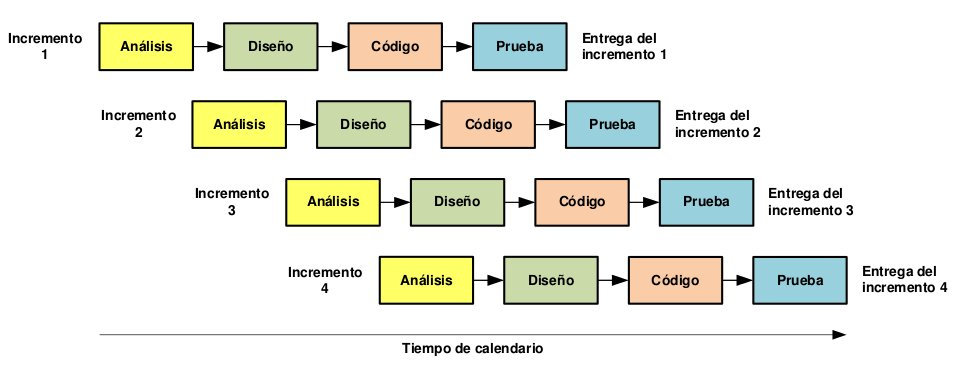
\includegraphics[width=1\linewidth]{imagenes/modelo_incremental}
	\caption{Imagen de la estructura del modelo incremental \cite{modeloIncremental}}
	\label{fig:modeloincremental}
\end{figure}

Este tipo de metodología permite realizar desarrollos o tareas en paralelo, para al final unirlo todo y que funcione correctamente. Una estructura así era necesaria, ya que para implementar cada uno de los gráficos disponibles, necesitaba su propio análisis, su adaptación del diseño original al de la aplicación, aplicar las técnicas de reducción apropiadas para cada gráfico, y su correspondiente tiempo de pruebas.

\section{Planificación}

Como se ha explicado en el apartado anterior, al seguir una metodología incremental durante el desarrollo de la API, permite agrupar las tareas en desarrollos independientes.

La primera tarea fue realizar el diseño base del circuito funcional de la herramienta, es decir, cual era la función de cada una de las herramientas que se iban a implementar y como se conectaban con el resto, para así lograr obtener un flujo de interacción entre todas. Establecido el diseño, el siguiente paso sería implementarlo y comprobar que el flujo de datos entre todas las aplicaciones y el resultado obtenido era el correcto.

Otra de las tareas que se desarrollaron el paralelo con el resto era el diseño de la lista de gráficos disponibles. Con el uso de la librería de gráficos D3JS, que se explicará más adelante, el siguiente paso era elegir que gráficos se iban a implementar, adaptarlos a la API y comprobar que se dibujaran correctamente.

También otra tarea importante fue el desarrollo de la interfaz web de la API. Diseñar una buena interfaz capaz de aprovechar la máxima potencia del núcleo de la aplicación, era una de las prioridades básicas. Con ella se puede acceder a todas las funciones de la API, configurar las distintas conexiones con las herramientas principales como \textit{MongoDB} \cite{MongoInicial}, \textit{Spark} o \textit{Hadoop} de manera sencilla, o tener la posibilidad de visualizar varios gráficos resultados para poder comparar entre ellos y mejorar el análisis de los datos.

La parte de testeo de la aplicación para comprobar los límites de la misma, fueron casi tres semanas de pruebas. En ella hubo que probar el rendimiento de la aplicación en situaciones reales, con grandes cantidades de datos, y comprobando el tiempo que podía tardar en procesarlo, si no había ningún error.

\section{Lenguajes de Programación y Herramientas}

Durante cada una de las tareas en cada fase, ha habido que aprender a utilizar herramientas y aprender programar en lenguajes, como es el caso de HTML, CSS y Javascript, para poder crear una interfaz web que se adapte a las funciones de la API, o como el caso de \textit{Scala}, lenguaje para programar las funciones de \textit{Spark}.

\subsection{Scala}
\begin{minipage}{\textwidth}
	\centering
	
\includegraphics[width=0.3\textwidth]{imagenes/scala_logo.jpg}\\[0.1cm]
\end{minipage}

Uno de los lenguajes más novedosos es \textbf{Scala}. Es un lenguaje de programación multi-paradigma cuya base está diseñada para programar con patrones. Además integra características de los lenguajes orientados a objetos y funcionales como Java \cite{ScalaInicial}. Al ser un lenguaje funcional, Scala permite desarrollar en una sintaxis ligera, definiendo funciones para realizar las operaciones e incluso anidarlas. 

Scala está basado en el paradigma MapReduce, que se comentó al comiendo del documento. Esto quiere decir que todos los procesamientos los puede realizar de manera paralela, aumentando la velocidad de cómputo.

Por todas las grandes características que ofrece, es el lenguaje elegido para programar las funciones de Spark, de entre todos los disponibles de la herramienta. Está perfectamente integrado con Spark y permite que la programación que se realice, sea muy escalable, tanto si se ejecuta sobre un ordenador como sobre un cluster, sin necesidad de cambiar nada de lo programado. 

En la API, se han programado en Scala todas las funciones de análisis de los datos que provienen de Hadoop, aplicando las técnicas de reducción de datos y esquemas de agrupación elegidos para el gráfico que se está desarrollando. Se adapta muy bien a la lectura de datos de tipo CSV o JSON, tipos de datos principales en la base de datos. 


\subsection{NodeJS}
\begin{minipage}{\textwidth}
	\centering
	
\includegraphics[width=0.4\textwidth]{imagenes/nodejs_logo.png}\\[0.1cm]
\end{minipage}

En la parte intermedia del diseño se encuentra \textbf{NodeJS} \cite{NodeJSInicial}. Está desarrollado en el lenguaje Javascript. Es un entorno de ejecución que gestiona las llamadas que se producen de manera asíncrona \cite{NodeJSAbout}. Esto permite manejar varias conexiones de manera concurrente sin la necesidad de que el usuario esté vigilando el bloqueo de procesos, como ocurre en las operaciones de redes basadas en hilos o hebras. Debido a que no hay bloqueos, es muy sencillo crear aplicaciones escalables en NodeJS.

Node mejora el modelo de eventos diseñados en otros sistemas, tratando el bucle de eventos como un entorno en vez de una librería. Su comportamiento se define a través de funciones callbacks, las cuales al inicio y final del script se inicia el servidor. En otros lenguajes, en las funciones callback se realiza una llamada de bloqueo, pero en NodeJS la añade al bucle de eventos después de ejecutar el script de entrada. Sale del bucle cuando no hay más funciones callbacks que ejecutar. Se puede apreciar un gráfico explicativo en la figura \ref{fig:nodejseventloop}.

\begin{figure}
	\centering
	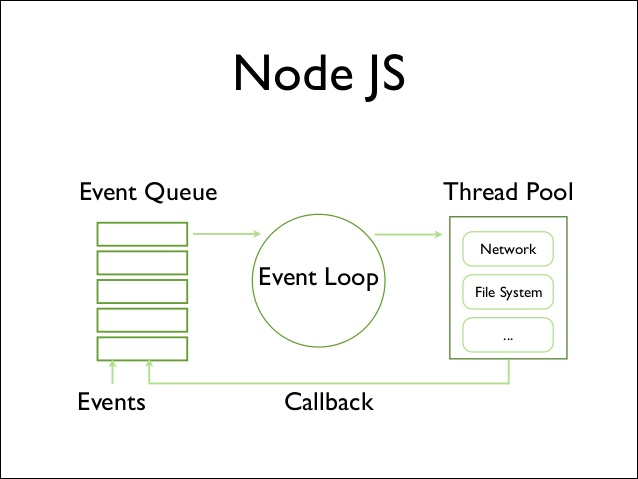
\includegraphics[width=0.9\linewidth]{imagenes/NodeJS_Event_Loop}
	\caption{Esquema del bucle de eventos de NodeJS \cite{NodeJSEventLoop}}
	\label{fig:nodejseventloop}
\end{figure}

Para la API desarrollada, NodeJS es una parte importante del sistema. Es la capa intermedia de la aplicación, donde se encarga de la comunicación entre la interfaz web del usuario con Hadoop, Spark y MongoDB. 
Además, se encarga también de configurar el servidor virtual donde se gestionan todas las peticiones. En este servidor se recogen las peticiones de representar un gráfico concreto, para unos datos y con unos parámetros específicos. Después se encarga de mandar a Spark la información solicitada por el usuario y, a continuación, espera a que el resultado esté disponible en MongoDB. Este se almacena en una base de datos en formato JSON, como ya se explicó en el apartado correspondiente a Mongo. Una vez obtenido, se encarga de dibujar el gráfico usando la librería D3JS.

\subsection{D3JS}
\begin{minipage}{\textwidth}
	\centering
	
\includegraphics[width=0.5\textwidth]{imagenes/d3js_logo.png}\\[0.1cm]
\end{minipage}

\textbf{D3JS} \cite{D3JSGithub} es una librería escrita en Javascript encargada de producir gráficos interactivos a partir de documentos basados en datos, como los ficheros de tipo CSV, TSV o JSON. La base para representar los gráficos de la librería D3JS es utilizar SVG, Canvas y HTML. Al estar escrito en Javascript, el lenguaje para darle funcionalidad a las páginas web, D3JS tiene la potencia para poder interactuar con los gráficos diseñados. De esta manera, las funciones de la librería permiten crear objetos de tipo SVG, darle efectos dinámicos o agregar información sobre el gráfico, o incluso seleccionar algunos de los elementos del infograma, pudiendo obtener otro como resultado de esa selección. 

D3JS se ha implementado como la librería para crear los gráficos de la API. En este caso, cada uno de los gráficos se genera a partir de obtener los resultados de los cálculos por parte de Spark, que están almacenados en MongoDB. Si bien, cada uno de los gráficos tiene puntos fuertes y débiles, por lo que es imprescindible la mano de un usuario experto en análisis de datos, para saber qué gráfico es el adecuado para los datos seleccionados a representar y con qué parámetros. Así se podrá obtener buenos resultados, que sean capaces de expresar lo que están contando los datos, ya que también es parte fundamental saber interpretar los infogramas.

\subsection{HTML, CSS y Javascript}
\begin{minipage}{\textwidth}
	\centering
	
\includegraphics[width=0.3\textwidth]{imagenes/HTML5_CSS_JavaScript_logo.png}\\[0.1cm]
\end{minipage}

Al estar escrita en Javascript la librería D3JS, lo mejor para aprovechar toda su potencia es crear una interfaz web para los usuarios finales. Esto permite poder acceder al sistema desde cualquier parte del mundo, desde cualquier dispositivo, de manera rápida y sencilla, a la vez que escalable. 

Con esta idea en mente, lo primordial es crear una interfaz que aproveche el máximo rendimiento de la aplicación, con un diseño elegante y sencillo. Para ello, se utilizó la plantilla \textbf{Gentelella} \cite{GentelellaGithub}, la cual incorpora muchas posibilidades para diseñar la web y una amplia gama de funcionalidad para cada uno de los paneles. 
Es una de las plantillas gratuitas que mejor se adapta a dispositivos tanto móviles como tablets. Además, trae varia funcionalidad para gestionar usuarios, lo que permite implementarlo en un futuro como una gran mejora del programa.


\subsection{GitHub}
\begin{minipage}{\textwidth}
	\centering
	
\includegraphics[width=0.4\textwidth]{imagenes/github_logo.png}\\[0.1cm]
\end{minipage}

Una de las herramientas fundamentales para todos los proyectos, es el gestor de versiones \textbf{GitHub}. Con ello se puede controlar cada una de las actualizaciones que se realizan del sistema, dando la posibilidad de volver atrás para comprobar cualquier estado anterior del mismo. Además permite gestionar las tareas a desarrollar mediante los \textit{Milestones}, reportar errores de funcionalidad, añadir mejoras a la aplicación o documentar cada una de las tareas. Pero la gran ventaja es que permite que otra gente pueda colaborar en el proyecto o controlar el proceso de desarrollo. 

Todas estas características han sido utilizadas durante el desarrollo de la API, haciendo más sencilla el control sobre la misma. También cabe destacar, que GitHub ha servido de puente para las actualizaciones entre los desarrollos en el ordenador local y el servidor donde se aloja el sistema.

\subsection{Docker}
\begin{minipage}{\textwidth}
	\centering
	
\includegraphics[width=0.4\textwidth]{imagenes/docker_logo.png}\\[0.1cm]
\end{minipage}

\textbf{Docker} \cite{DockerInicial} es una plataforma abierta, usada por desarrolladores y administradores de sistemas, para desplegar aplicaciones dentro de contenedores aislados del sistema operativo.
Para realizar el desarrollo y pruebas correspondientes de la API, se ha utilizado Docker como herramienta para desplegar el sistema en los servidores de la ETSIIT durante todo el proceso.

\subsection{Lucidchart}
\begin{minipage}{\textwidth}
	\centering
	
\includegraphics[width=0.4\textwidth]{imagenes/lucidchart_logo.png}\\[0.1cm]
\end{minipage}

\textbf{Lucidchart} \cite{LucidchartInicial} es una herramienta para el diseño de diagramas de flujo a nivel profesional. Permite compartir los diseños para colaborar entre usuarios en tiempo real. Se pueden crear desde diagramas de flujo hasta diseños UML, pasando por una amplia variedad de tipos de diagramas. 

En esta ocasión, se ha utilizado Lucidchart para el diseño de la mayoría de las figuras de este documento donde se explica algunos de los funcionamientos del sistema. 

\subsection{LaTeX}
\begin{minipage}{\textwidth}
	\centering
	
\includegraphics[width=0.3\textwidth]{imagenes/latex_logo.png}\\[0.1cm]
\end{minipage}

\textbf{LaTeX} es un sistema de composición de textos orientado a la gran calidad tipográfica. Debido a esta característica y sus amplias posibilidades (por ejemplo, facilidad de escritura de expresiones matemáticas) es muy usado en el ámbito científico y académico. Por esta razón,  TeXstudio \cite{TexstudioInicial} ha sido el editor de texto seleccionado para escribir este documento LaTeX.




\chapter{Especificación de Requisitos Funcionales y No Funcionales}

\section{Requisitos funcionales}
Los requisitos funcionales de una herramienta o aplicación, describen cualquier comportamiento o funcionalidad concreta de la misma, bajo ciertas circunstancias. De una manera genérica, los requisitos funcionales deben incluir las acciones que realizan las pantallas específicas de la interfaz o describir cada uno de los flujos de datos y computo de cada una de las capas de la herramienta.

En este apartado, se van a dividir los requisitos funcionales en distintos grupos según la capa del software.

\subsection{Requisitos funcionales de cómputo (Nivel inferior)}
Lo primero de todo es comprobar que funcionalidad se realiza en el nivel más inferior del sistema. Esto permitirá tener una idea global de lo que hace el sistema. 
\begin{itemize}
	\item Cuando se ejecuta uno de los paquetes que contienen el código fuente para realizar los cálculos de cada uno de los gráficos, o el paquete para obtener un resumen sobre un fichero, lo primero que hace Spark es buscar dicho archivo, en la ruta especificada, dentro del HDFS.
	\item Los archivos que contiene los datos deben ser tipo CSV.
	\item La conexión Spark-Hadoop se realiza mediante una librería específica para realizar estas acciones, dentro de Spark.
	\item Una vez recuperado el archivo, el siguiente paso es transformarlo en un Dataframe, la estructura con la que trabaja Spark para tratar los datos.
	\item Antes de continuar con los cálculos, se crean las estructuras que almacenarán los datos resultados en formato JSON, dependiendo del paquete que se esté ejecutando.
	\item A continuación, se aplica el esquema de agrupación y la técnica de reducción de datos elegida para cada uno de los gráficos.
	\item En el caso de la librería encargada de extraer los datos resumen o ‘summary’, se encarga de obtener datos propios del archivo como el número de columnas, el número de filas, el peso del archivo o los nombres de todas las columnas.
	\item Una vez obtenidos los resultados, estos se almacenan en las estructuras indicadas anteriormente. 
	\item Después, se realiza la comunicación entre Spark y MongoDB para guardar estos resultados dentro de una base de datos y colección indicados en los parámetros.
\end{itemize}

\subsection{Requisitos funcionales de comunicación (Nivel intermedio)}
\begin{itemize}
	\item El sistema se encargará de crear el servidor virtual donde se gestionarán todas las peticiones por parte de la interfaz web.
	\item Todas las peticiones que recibe se gestionan de manera asíncrona, lo que permite realizar múltiples acciones a la vez.
	\item Los parámetros de conexión con Hadoop, Spark y MongoDB están configurados en este nivel y, por el momento, solo son accesibles a través de código.
	\item Cuando el sistema solicite obtener el contenido de un path especifico dentro del HDFS de Hadoop, NodeJS enviará una solicitud a la API RESTful de Hadoop, donde se obtiene como resultado un listado, en formato JSON, de todos los documentos y directorios que existen dentro del indicado, con información importante de cada uno.
	\item Esta información devuelta será mostrada en los campos indicados para ello en la interfaz web.
	\item Cuando se solicite un nuevo gráfico en la interfaz web, se recogerá como una petición asíncrona de tipo 'get'.
	\item Justo después, se creará un identificador para cada una de las solicitudes de gráficos, compuesta por la ruta del archivo, el peso del mismo, el gráfico seleccionado y los parámetros.
	\item Cada una de las variables que componen el identificador, se encripta utilizando MD5. 
	\item Se debe crear un documento de tipo JSON, que se almacenará en una colección dentro de la base de datos de MongoDB, el cual servirá para mantener información, como la hora de inicio y fin de la ejecución o el gráfico indicado, sobre los documentos solicitados y los resultados de los gráficos y de los datos proporcionados por ‘summay’. 
	\item Este identificador también se envía como parámetro al nivel inferior, para que pueda ser identificado el resultado de la agrupación devuelto por Spark.
	\item Según indique el usuario en la interfaz, este mismo resultado puede ser representado de manera gráfica o directamente visualizar los datos en formato JSON. 
	\item Si el usuario solicita un gráfico que ya ha sido generado anteriormente, el sistema no volverá a realizar el cálculo sobre el fichero indicado, sino que buscará primero con el identificador si ya está cargado en la base de datos de MongoDB el resultado, o si otro usuario lo ha solicitado pero todavía no está completado. En cuyo caso, deberá esperar hasta que esté disponible para recoger el resultado y pintar el gráfico.
\end{itemize}

\subsection{Requisitos funcionales de la interfaz gráfica (Nivel superior)}
Como se puede apreciar en la figura \ref{fig:interfazinicial}, la interfaz del usuario final es bastante sencilla y simple de usar. Toda la funcionalidad gráfica se muestra en una sola pantalla, para simplificar la búsqueda de los elementos.
\begin{figure}
	\centering
	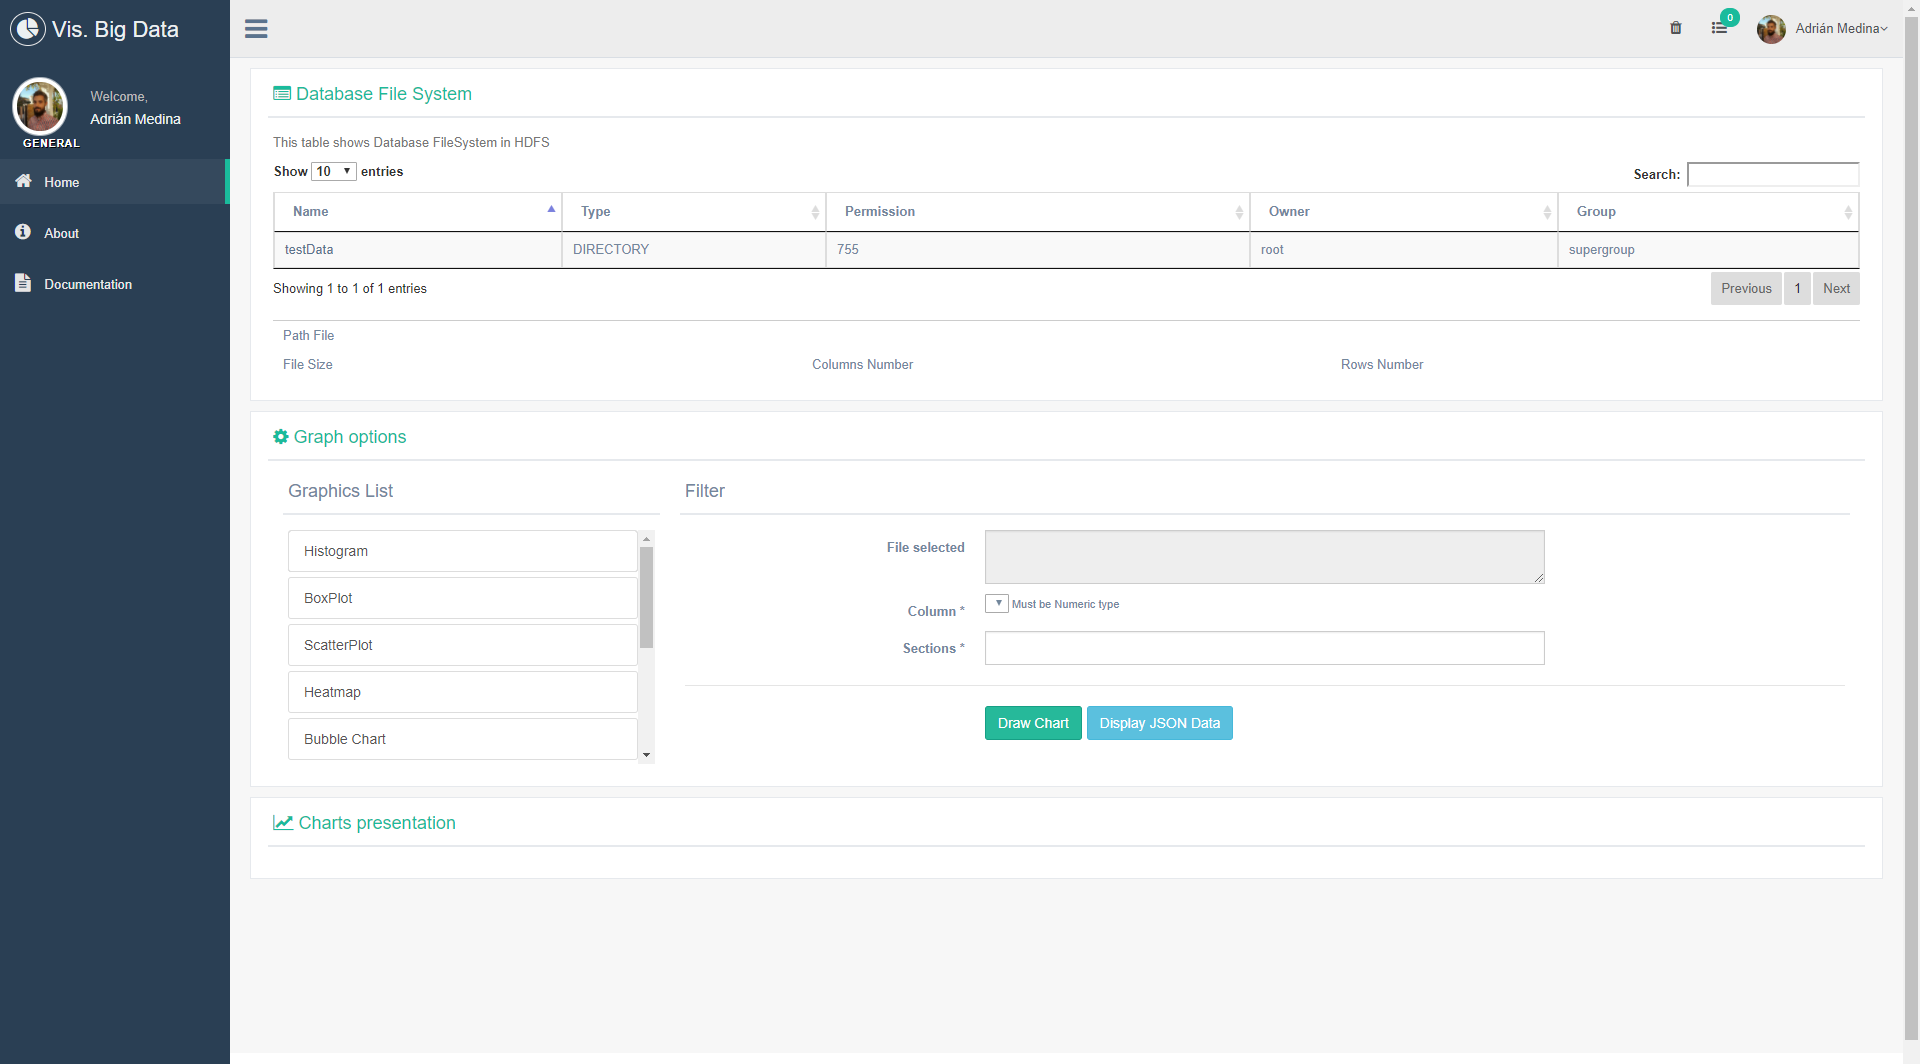
\includegraphics[width=1\linewidth]{imagenes/interfaz_inicial}
	\caption{Vista inicial de la interfaz web de la API}
	\label{fig:interfazinicial}
\end{figure}
\begin{figure}
	\centering
	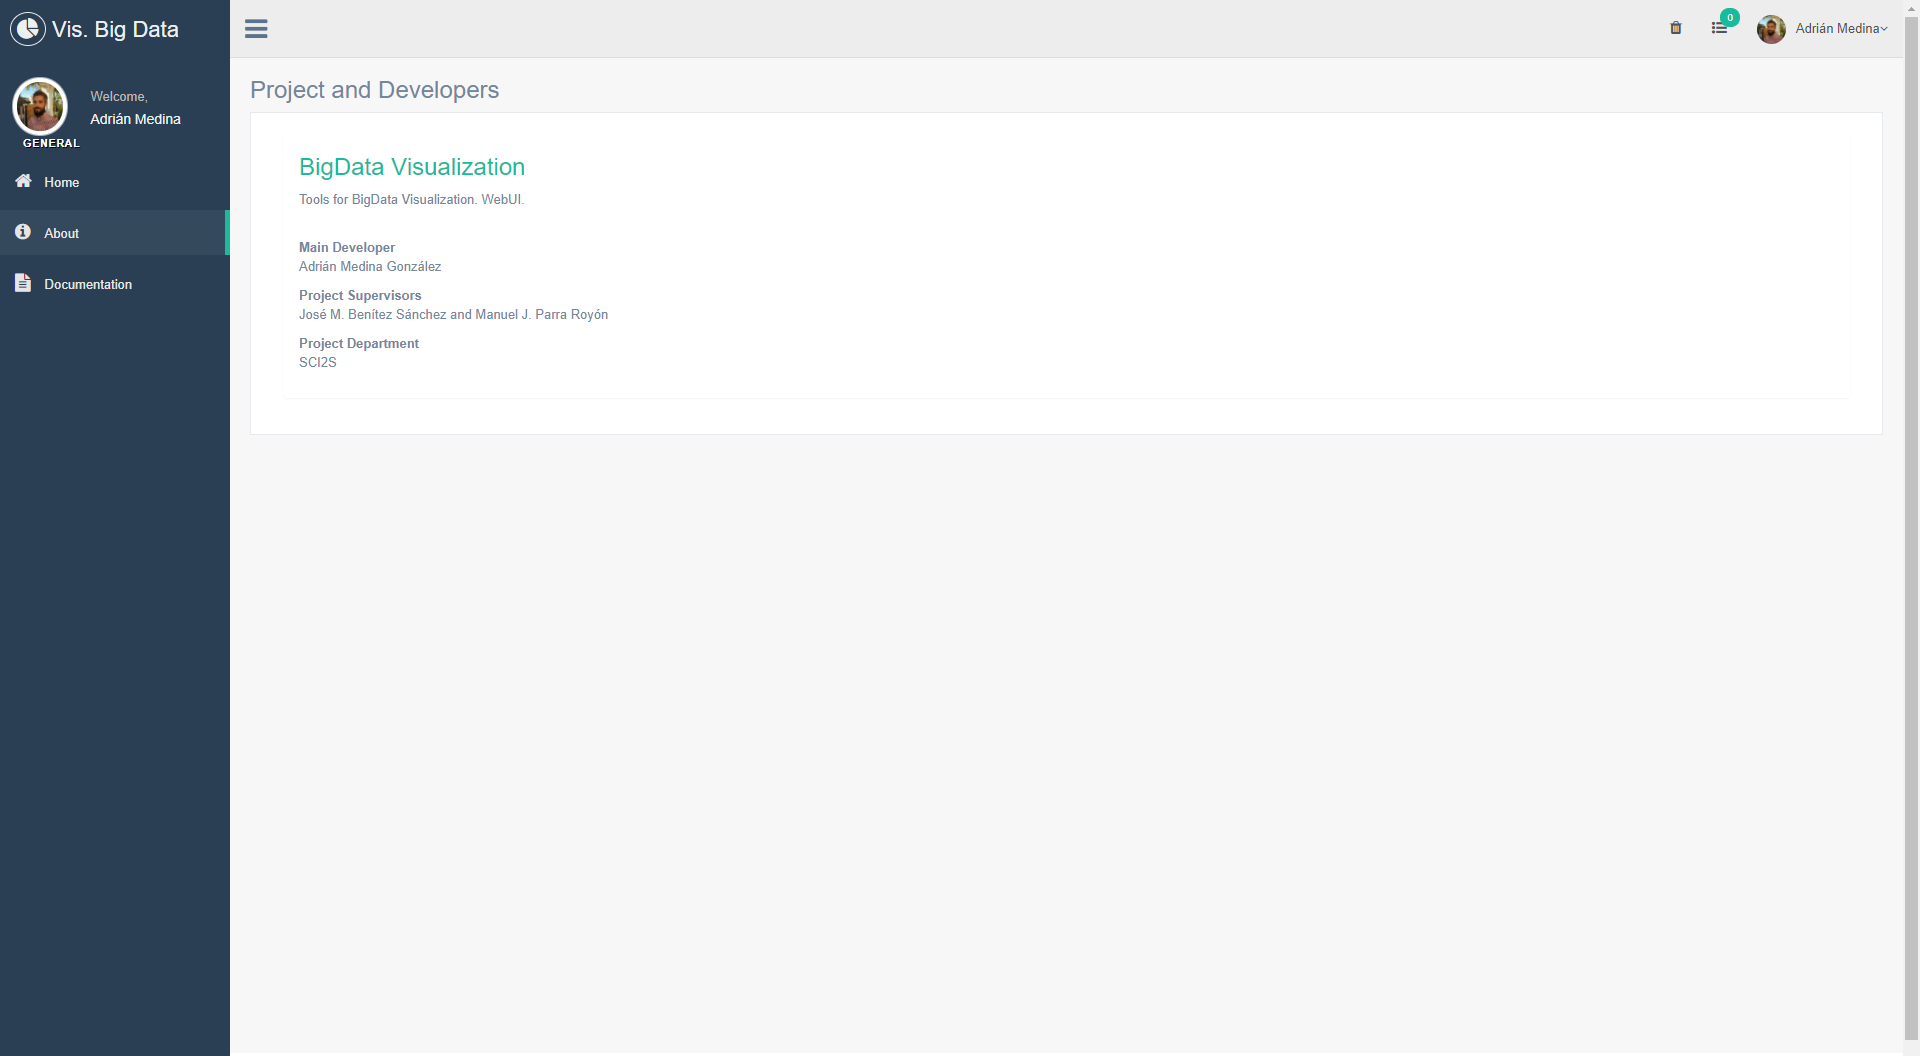
\includegraphics[width=1\linewidth]{imagenes/boton_about}
	\caption{Información sobre el proyecto}
	\label{fig:botonabout}
\end{figure}
\begin{figure}
	\centering
	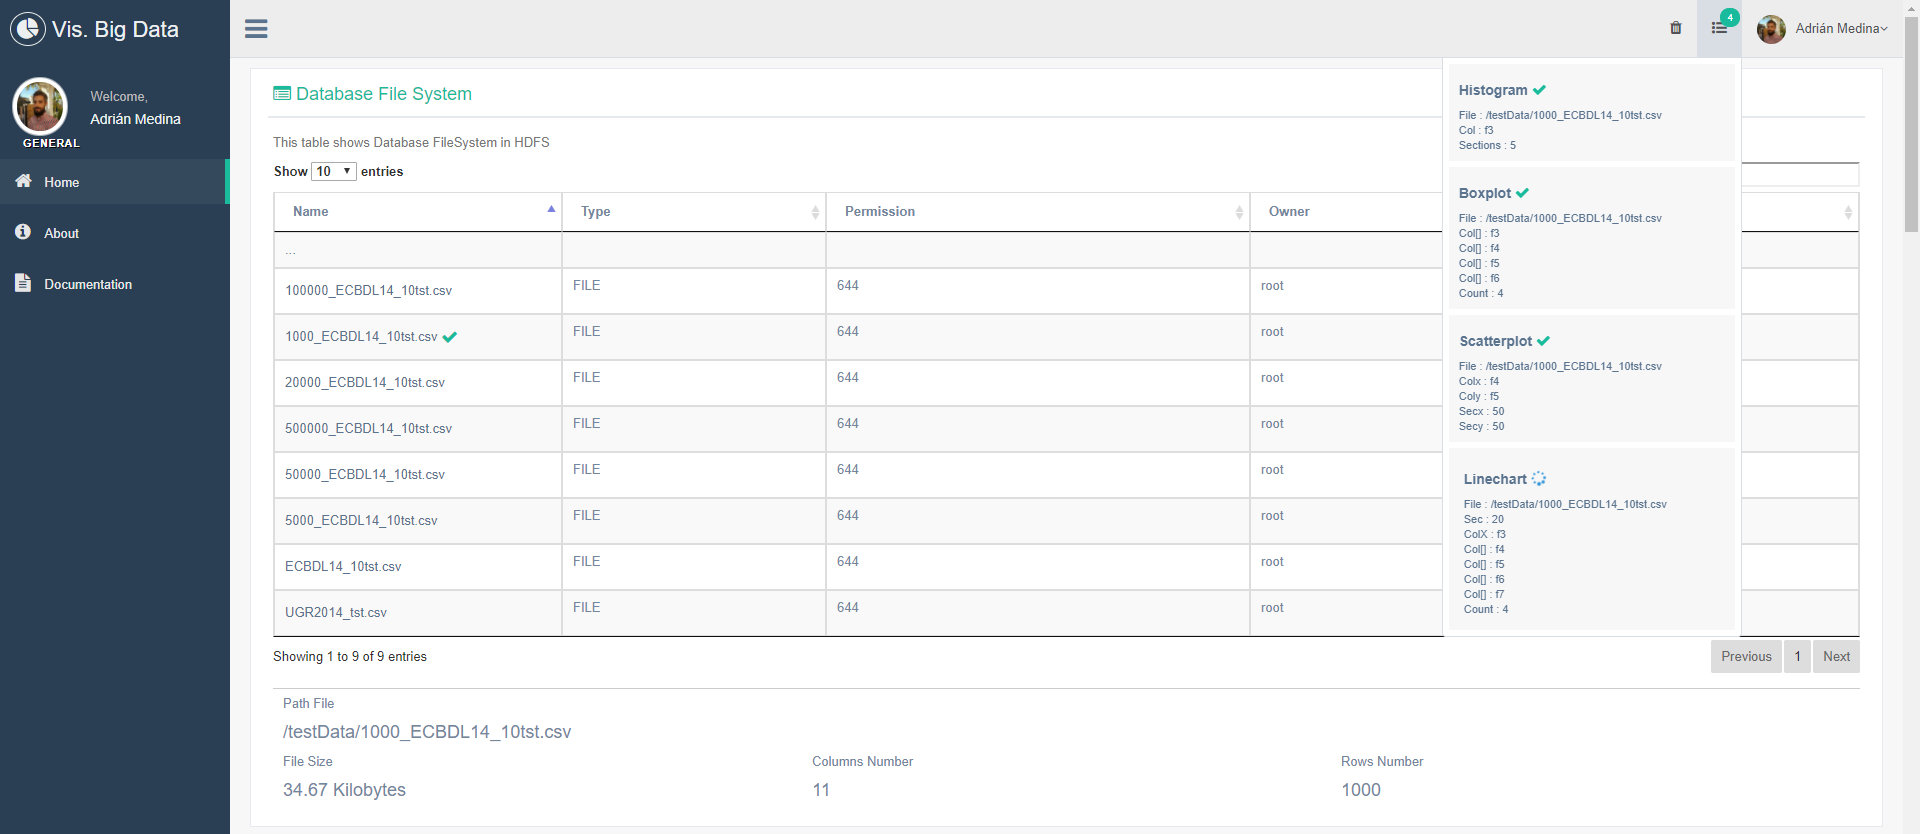
\includegraphics[width=1\linewidth]{imagenes/lista_ultimos_graficos}
	\caption{Listado de los últimos gráficos generados}
	\label{fig:listaultimosgraficos}
\end{figure}

\begin{itemize}
	\item Al cargar la interfaz, el sistema cargará automáticamente el contenido del directorio raíz del HDFS, en la sección indicada para ello.
	\item En esta tabla se muestra información de los archivos y directorios de la ruta actual, como el nombre, si es un directorio o un archivo, los permisos que tiene dentro del HDFS, el usuario propietario y el grupo al que pertenece.
	\item Cada uno de los botones de la cabecera de la tabla permite ordenar el contenido de manera ascendente o descendente.
	\item Hay un menú desplegable donde se puede indicar el número de documentos que se desean visualizar en la tabla.
	\item Si hubiera más elementos de los indicados, el gestor de páginas de la tabla permite navegar entre las distintas listas de registros.
	\item En el campo ‘Search’, se puede buscar un registro concreto haciendo coincidir parte de la cadena que se escriba en el campo con algún contenido de los registros, de cualquier columna, ya sea el nombre, propietario o grupo, por ejemplo. Solo buscará los ficheros o directorios que se encuentren en el directorio actual que se está mostrando.
	\item Si el registro es un directorio, al hacer click en él, el sistema se encargará de obtener el contenido del mismo y actualizar la tabla con los nuevos registros.
	\item Por el contrario, si se trata de un fichero de tipo CSV, mandará a NodeJS la petición de obtener el resultado de ejecutar ‘summary’.
	\item Si se trata de un fichero de otro tipo o el fichero seleccionado se encuentra vacío, el sistema mostrará un mensaje de error indicando que es un fichero invalido.
	\item El resultado de ‘summary’ se mostrará en los campos habilitados para ello (justo debajo de la tabla donde se muestran los registros del HDFS).
	\item En el panel ‘Graph options’, el sistema muestra una lista de todos los gráficos disponibles en la herramienta. 
	\item Al seleccionar uno, el sistema habilitará un formulario para rellenar con los parámetros que necesita ese gráfico para calcular el resultado del nivel inferior.
	\item El sistema rellenará automáticamente los campos de ‘File selected’ y los campos de las columnas y ejes, con los datos obtenidos al seleccionar un fichero en la tabla del HDFS.
	\item Una vez relleno el formulario, al pinchar en el botón ‘Draw Chart’, se le comunicará a NodeJS la petición con los parámetros indicados, y devolverá el gráfico resultado en el panel ‘Charts presentation’. 
	\item Si por el contrario seleccionamos el botón ‘Display JSON Data’, en vez de dibujar el gráfico, mostrará los datos en formato JSON.
	\item En este último panel, se pueden acumular tantos gráficos como se ejecuten, con la posibilidad de comparar varios a la vez, teniendo la posibilidad de cerrar alguno haciendo click en el símbolo ‘X’ de la esquina superior derecha.
	\item En la parte superior de la pantalla, el sistema almacena una lista tanto con los últimos gráficos que se han generado como los que se están ejecutando actualmente, como se puede apreciar en la figura \ref{fig:listaultimosgraficos}. De esta manera, si se selecciona uno que ya esté finalizado, el sistema ejecutará de nuevo el gráfico con los mismos parámetros sin la necesidad de volver a introducirlos a mano.
	\item El botón justo a la izquierda, con el icono del cubo, ejecuta la función de limpiado de la lista, si después de ejecutar muchos gráficos, el usuario necesita tenerla vacía.
	\item También arriba a la derecha se encuentra información sobre el usuario y algunas de las acciones que se podrán hacer, cuando se implemente en un futuro la gestión de usuarios.
	\item En el menú lateral izquierdo, el botón ‘Home’ y el título del proyecto justo encima, ejecuta la pantalla principal con el contenido descrito anteriormente.
	\item El botón ‘About’, muestra información acerca del proyecto, como una breve descripción de la funcionalidad de la API, su desarrollador principal o supervisores del proyecto, tal y como se muestra en la figura \ref{fig:botonabout}.
	\item El botón 'Documentation' abre una nueva ventana con la API RESTful que proporciona Swagger, donde se puede obtener información acerca de todas las funcionalidades del sistema, como se puede apreciar en la figura \ref{fig:swaggerfunciones}.
	\item Si se selecciona una de las funciones, se puede ejecutar para obtener el resultado en formato JSON, indicándole los parámetros necesarios, tal y como se puede ver en un ejemplo sobre la función encargada del histograma en la figura \ref{fig:swaggerhistograma}.
	\item Al hacer click en cualquiera de los botones del menú lateral izquierdo, el sistema hace una recarga de la página para mostrar su contenido.
\end{itemize}

\begin{figure}
	\centering
	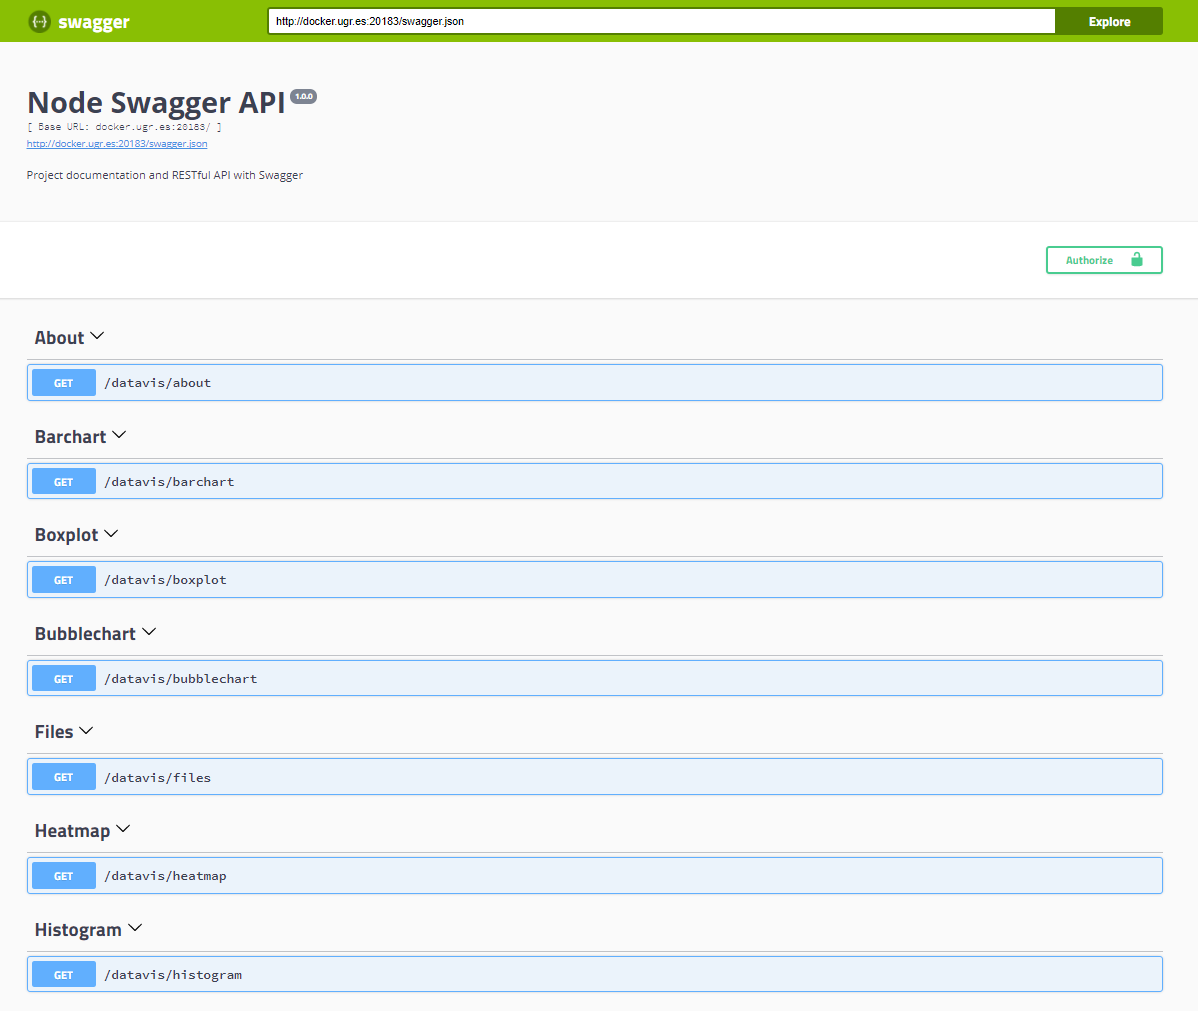
\includegraphics[width=1\linewidth]{imagenes/swagger_funciones}
	\caption{Funciones a través de Swagger}
	\label{fig:swaggerfunciones}
\end{figure}
\begin{figure}
	\centering
	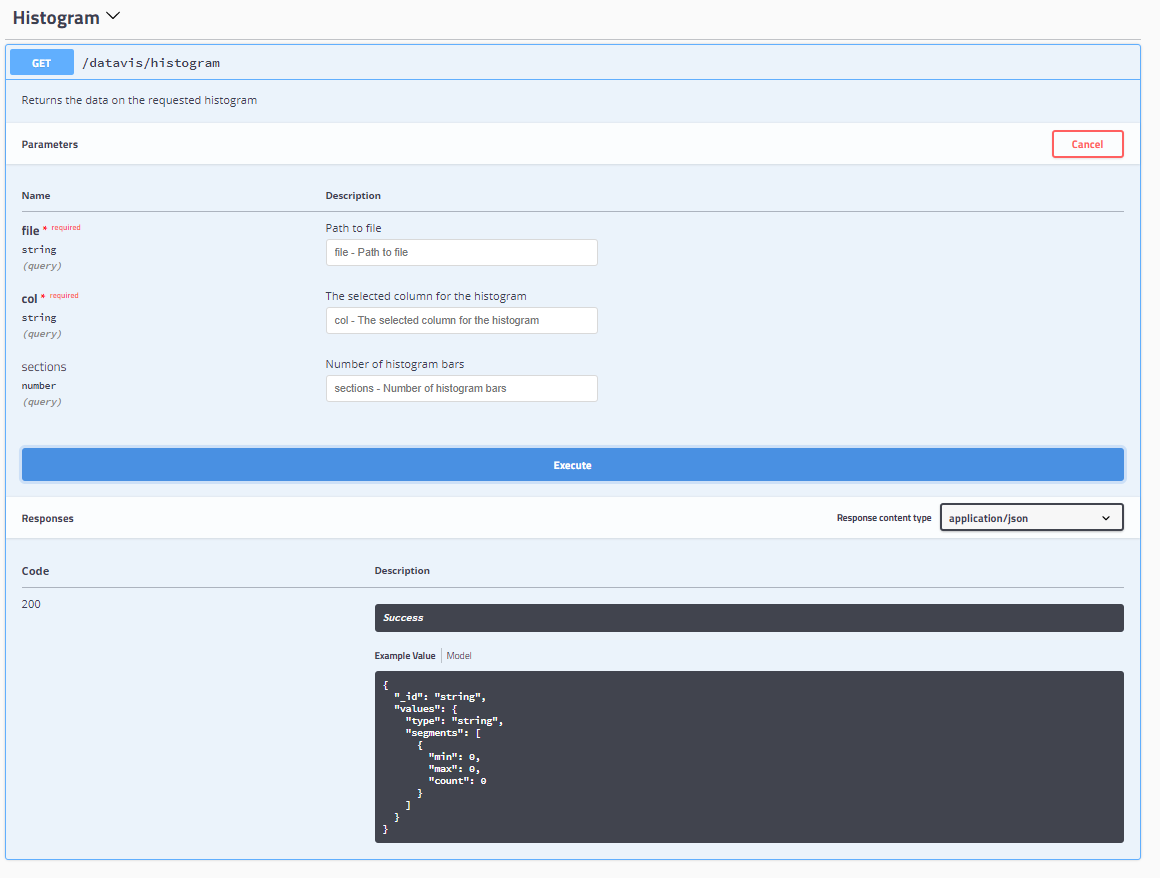
\includegraphics[width=1\linewidth]{imagenes/swagger_histograma}
	\caption{Función histograma en Swagger}
	\label{fig:swaggerhistograma}
\end{figure}

\section{Requisitos no funcionales}
Los requisitos no funcionales representan características de funcionamiento y algunas restricciones del sistema que se está implementando. Estos requisitos no se refieren al comportamiento específico de las funciones del sistema, sino características del propio sistema como la concurrencia, la escalabilidad o eficiencia. De esta forma, podemos agruparlos según las características.

\subsection{Eficiencia}
\begin{itemize}
	\item El sistema debe ejecutar las peticiones de manera asíncrona, por lo que permite usar la herramienta en varios dispositivos, obteniendo cada uno sus propios resultados.
	\item Por la misma razón, el sistema debe ser capaz de operar con muchos usuarios al mismo tiempo de manera fluida.
	\item Si el cálculo de un gráfico concreto, sobre el mismo fichero y con los mismos parámetros ya ha sido ejecutado anteriormente, entonces no volverá a realizar la misma operación, agilizando así la fluidez con la que se obtienen los resultados en la API.
	\item El sistema debe cargar de manera veloz los directorios del HDFS de Hadoop, para no aumentar los tiempos de espera de la API.
	\item Todos los cambios que se realicen sobre los ficheros en el HDFS, deben estar listos al instante para poder generar los gráficos con los nuevos datos.
	\item El sistema debe ser capaz de recibir y ejecutar varias peticiones a la vez sin problemas.
	\item Spark y Scala deben aprovechar al máximo los recursos del ordenador o cluster disponibles al permitir dividir y ejecutar los procesos en paralelo.
\end{itemize}

\subsection{Escalabilidad}
\begin{itemize}
	\item Al estar montado el sistema sobre herramientas fácilmente escalables como Hadoop o Spark, debe permitir instalarlo y ejecutarlo sobre cualquier ordenador o cluster, tanto en el aumento de nodos como en su decremento.
	\item Por el mismo motivo anterior, al cambiar de componentes hardware debe seguir funcionando perfectamente, siempre que cumpla los requisitos mínimos del sistema.
\end{itemize}

\subsection{Seguridad de los datos}
\begin{itemize}
	\item El sistema tiene copias de seguridad gracias a la estructura de almacenamiento de datos de Hadoop gracias a HDFS.
	\item Los datos resultados permanecen en MongoDB con su correspondiente documento con información acerca del estado de los mismos.
\end{itemize}

\subsection{Accesibilidad}
\begin{itemize}
	\item El sistema tiene compatibilidad con cualquier navegador web actualizado en sus últimas versiones.
	\item También la interfaz está diseñada para adaptarse a los tamaños de los dispositivos móviles o tablets, actualizados recientemente.
\end{itemize}

\subsection{Requisitos hardware}
\begin{itemize}
	\item Es necesario tener instaladas y configuradas las herramientas Hadoop, Spark, MongoDB y NodeJS
	\item El sistema debe poder lanzar el HDFS de Hadoop en el sistema, que requiere como mínimo 8 GB de RAM.
	\item Como mínimo, el sistema ocupa cerca de los 4GB de disco.
	\item En el caso de Spark y MongoDB, los requisitos hardware son los configurados para estas herramientas, ya que se puede ejecutar desde un ordenador hasta un cluster. 
\end{itemize}

\subsection{Versiones}
\begin{itemize}
	\item El sistema debe tener instalado una versión de Java JDK igual o superior a 1.7.0
	\item La versión de Scala debe ser 2.11
	\item Para Hadoop, tener instalado como mínimo la versión 2.6
	\item Se ha configurado Spark para utilizar una versión igual o superior a 2.0
	\item Debe instalarse y configurarse igual o superior de MongoDB a la 3.2
	\item Para NodeJS, la versión debe ser 6.9 o superior
	\item También es necesario tener otras aplicaciones secundarias como Sbt, Swagger y Forever para el correcto funcionamiento de la aplicación.
\end{itemize}



\chapter{Diseño del Sistema}

\section{Diseño de la arquitectura del sistema}
Establecer el ámbito de las tareas que realiza la API, es el primer paso para conseguir un buen diseño de la arquitectura. Conocer a priori en qué momento se ejecutan cada una, es lo que ayuda a clasificarlas de alguna manera. Dicho esto, se pensó que lo mejor era dividir el programa se divide en tres niveles o capas, superior o de interfaz, intermedia o de comunicación, e inferior o de procesamiento, como se puede apreciar en la figura \ref{fig:arquitecturadelsistema}. 

\begin{figure}
	\centering
	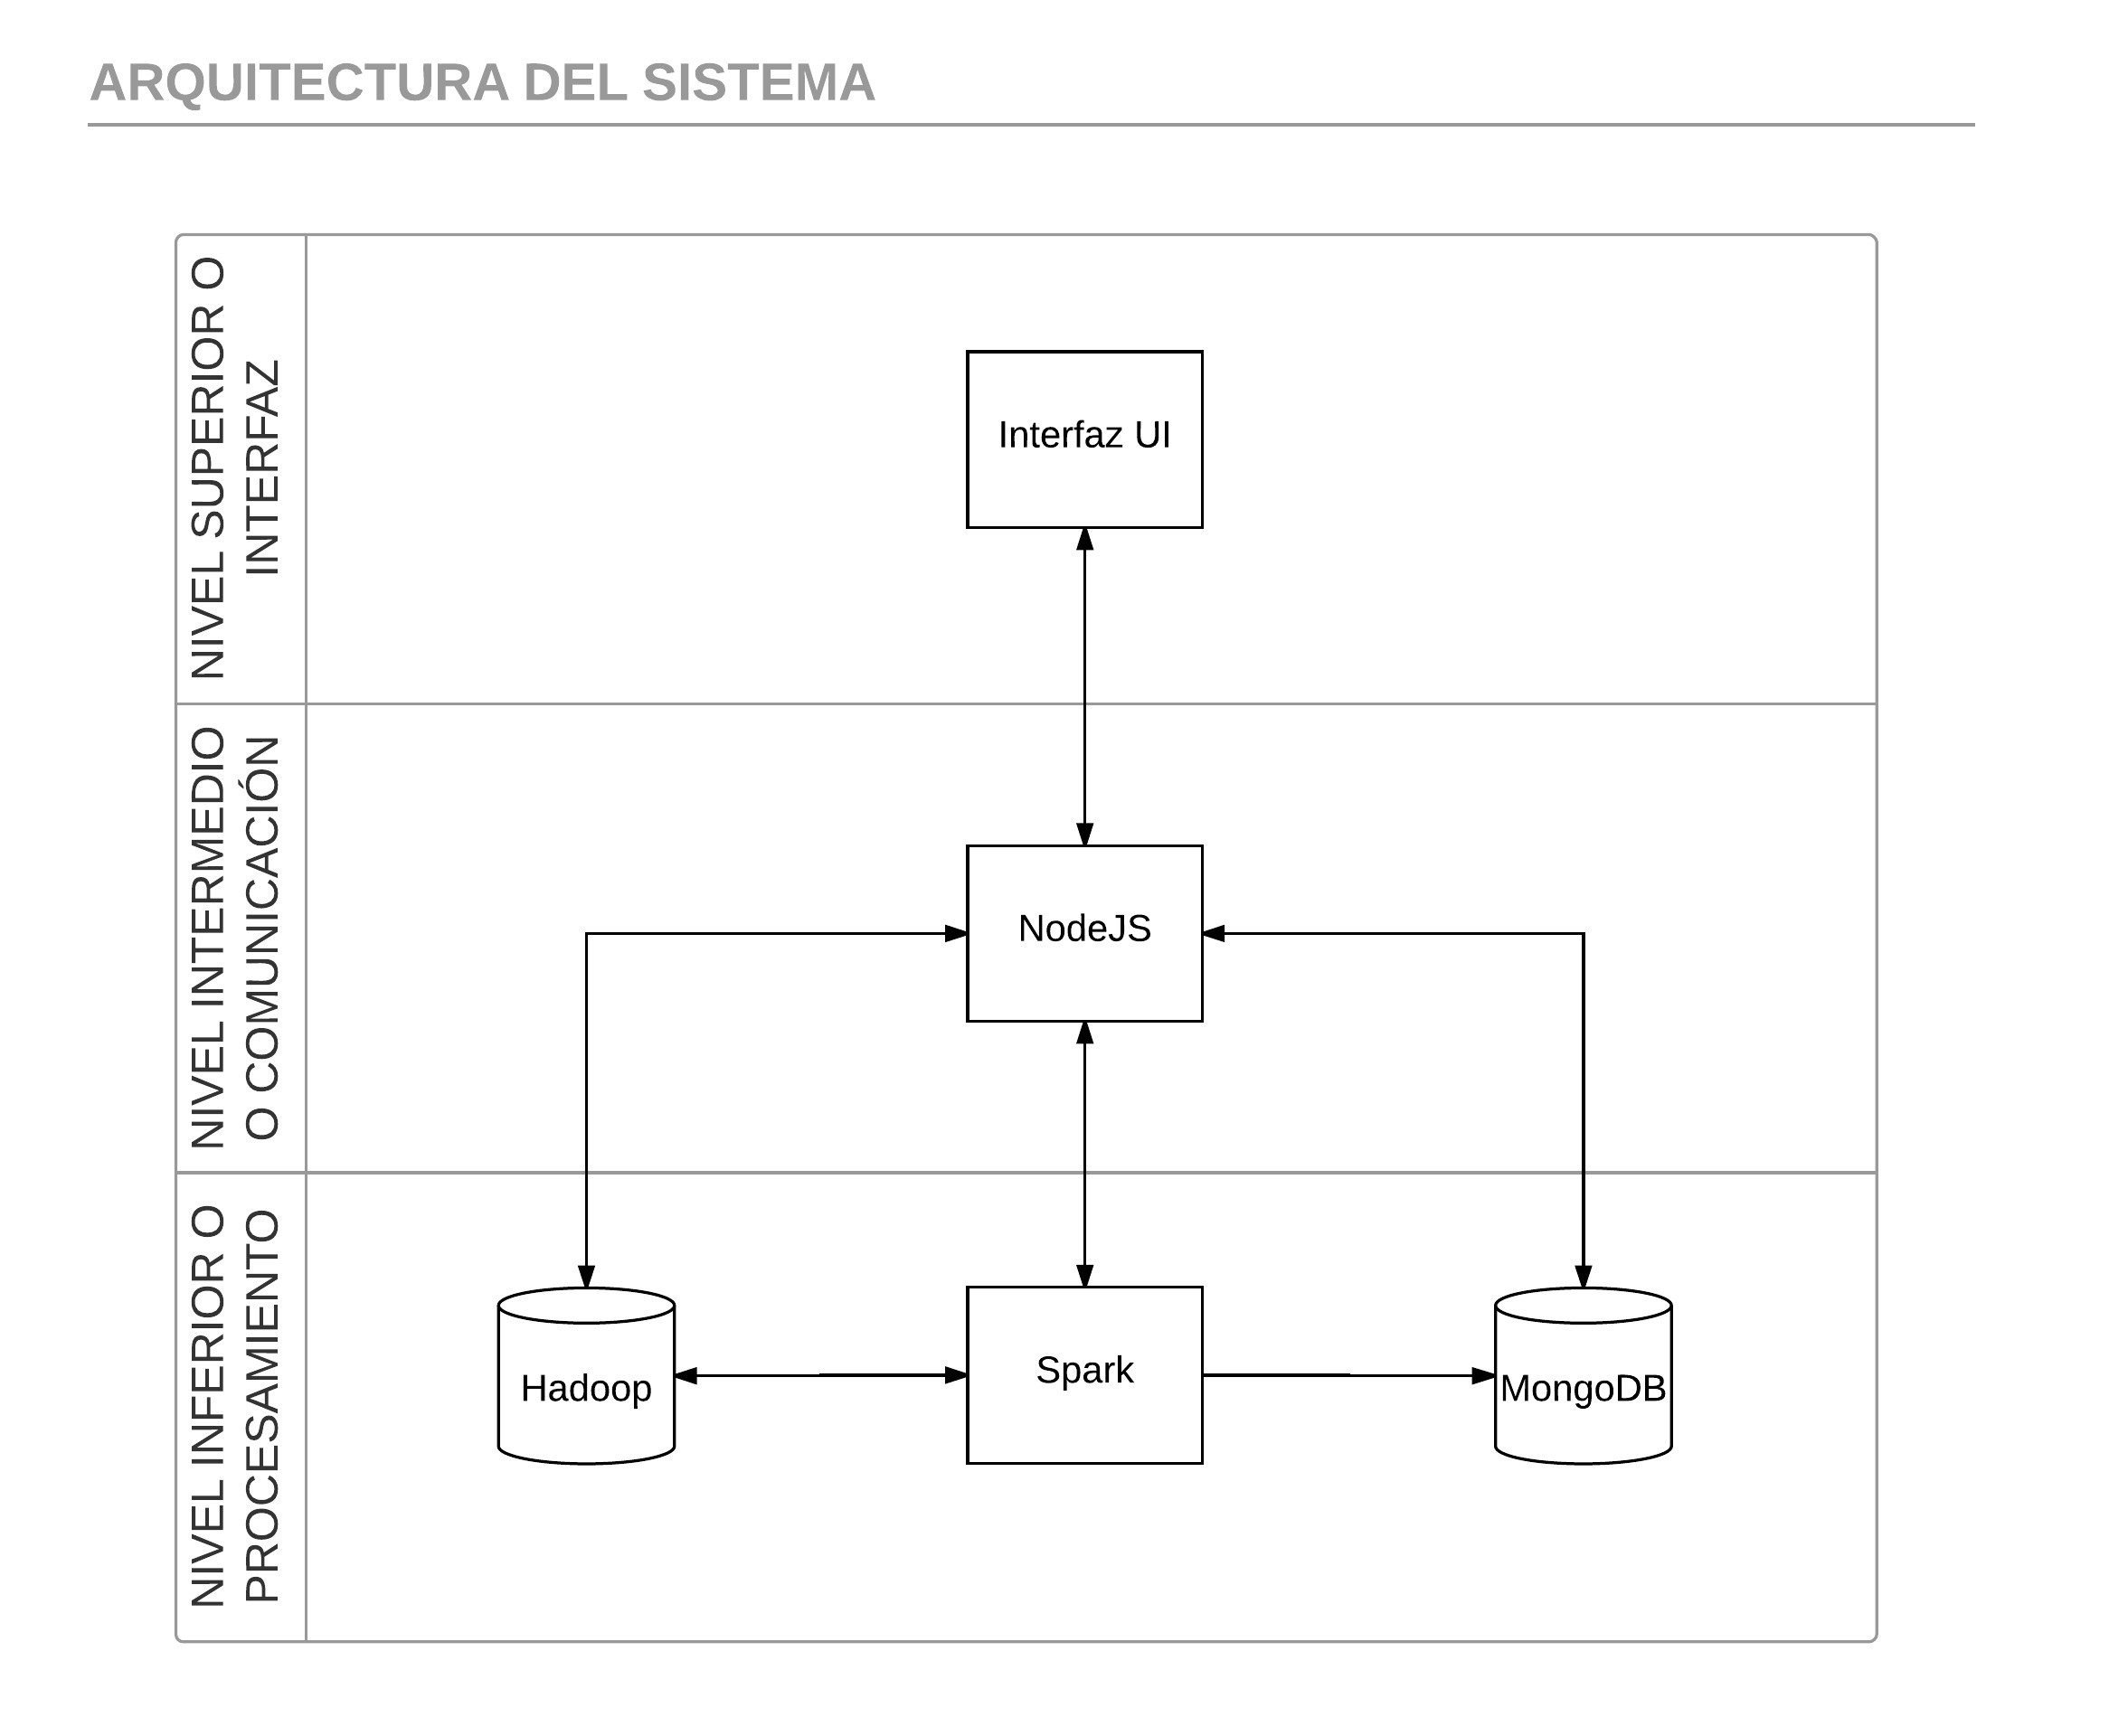
\includegraphics[width=1\linewidth]{imagenes/Arquitectura_del_sistema}
	\caption{Diseño de la arquitectura del sistema}
	\label{fig:arquitecturadelsistema}
\end{figure}

El nivel superior o nivel de interfaz, es el encargado de comunicarse directamente con el usuario de la aplicación. En él, se aloja la parte web con la que trabajan los usuarios, permitiendo recoger la información que solicitan, para después, enviarla al nivel intermedio. La interfaz de la API está diseñada para poder trabajar con varios usuarios de manera concurrente, o poder trabajar sobre varias pestañas o ventanas una sola persona. Toda la funcionalidad de esta capa está escrita en Javascript, haciendo que la interfaz sea dinámica. Como se pudo ver en el capítulo anterior, la figura \ref{fig:interfazinicial} muestra el diseño de esta interfaz.

En el nivel intermedio o de comunicación, es donde se realiza toda la comunicación entre las distintas herramientas y hace que el flujo de datos entre la capa superior y la inferior sea el correcto. Aquí es donde se ejecuta NodeJS, siendo el encargado de recoger todos los tipos de eventos y acciones que se producen en la capa superior, para a continuación, realizar la solicitud de procesamiento de la información recibida a la capa inferior donde se encuentra Spark. Se puede decir que es el corazón del sistema, donde se gestiona toda la información y también es el encargado de crear el servidor virtual permitiendo que la aplicación pueda funcionar a través de un navegador web. 
También se encarga de la comunicación con MongoDB para obtener los resultados devueltos por Spark, para a continuación, dibujar el gráfico solicitado y después mandarlo a la capa superior, utilizando para ello la librería D3JS. 

Por último, en el nivel inferior o de procesamiento, se aplican los esquemas de agrupación y las técnicas de reducción elegidas para cada uno de los gráficos disponibles en la API. En este nivel es donde se alojan las herramientas Hadoop, Spark y MongoDB. Cada una de ellas tiene su propia función dentro del nivel, siendo así Hadoop el encargado de almacenar y mantener los datos del sistema, Spark el encargado de coger el fichero del HDFS, procesando los datos aplicando los esquemas de agrupación y las técnicas de reducción elegidas para cada uno de los gráficos disponibles en la API, y por parte de MongoDB, guardar el resultado enviado del procesado de Spark, manteniendo información acerca del estado de cada uno de los resultados, como la fecha de inicio de solicitud, o la de finalizado el cálculo, además de información acerca de si se está ejecutando en un instante preciso o ha finalizado. Esto ayuda para conocer si se está procesando ya un gráfico con unos parámetros y fichero de datos concreto, y se vuelve a solicitar, no volver a realizar el cálculo, sino esperar a que ese termine para devolver el resultado a la capa de comunicación.

\section{Conexión entre módulos}
En esta sección se va a explicar cómo se han conectado cada uno de los diferentes módulos o programas para que puedan comunicarse entre sí y que realicen su función de manera autónoma. Para ello, se va a dividir y explicar cada una de las conexiones. Algunos de las librerías que se utilizan para conectar los sistemas, deben añadirse con ayuda del gestor de paquetes ‘Sbt’ para poder utilizarlo en el código, y en el caso de NodeJS, se utiliza el gestor ‘NPM’.

\subsection{Hadoop - Spark}
La conexión entre estas dos herramientas viene integrada en el propio Spark. Es tan sencillo como crear el sqlContext a partir del SparkConfig, que viene en el paquete ‘Spark-sql’ y utilizar el método ‘read’ que trae la propia aplicación, pasándole como parámetro la URL donde se aloja el fichero en el HDFS. En la figura \ref{fig:conexionhadoopspark}, se muestra el flujo de llamadas entre las dos herramientas.

\begin{figure}
	\centering
	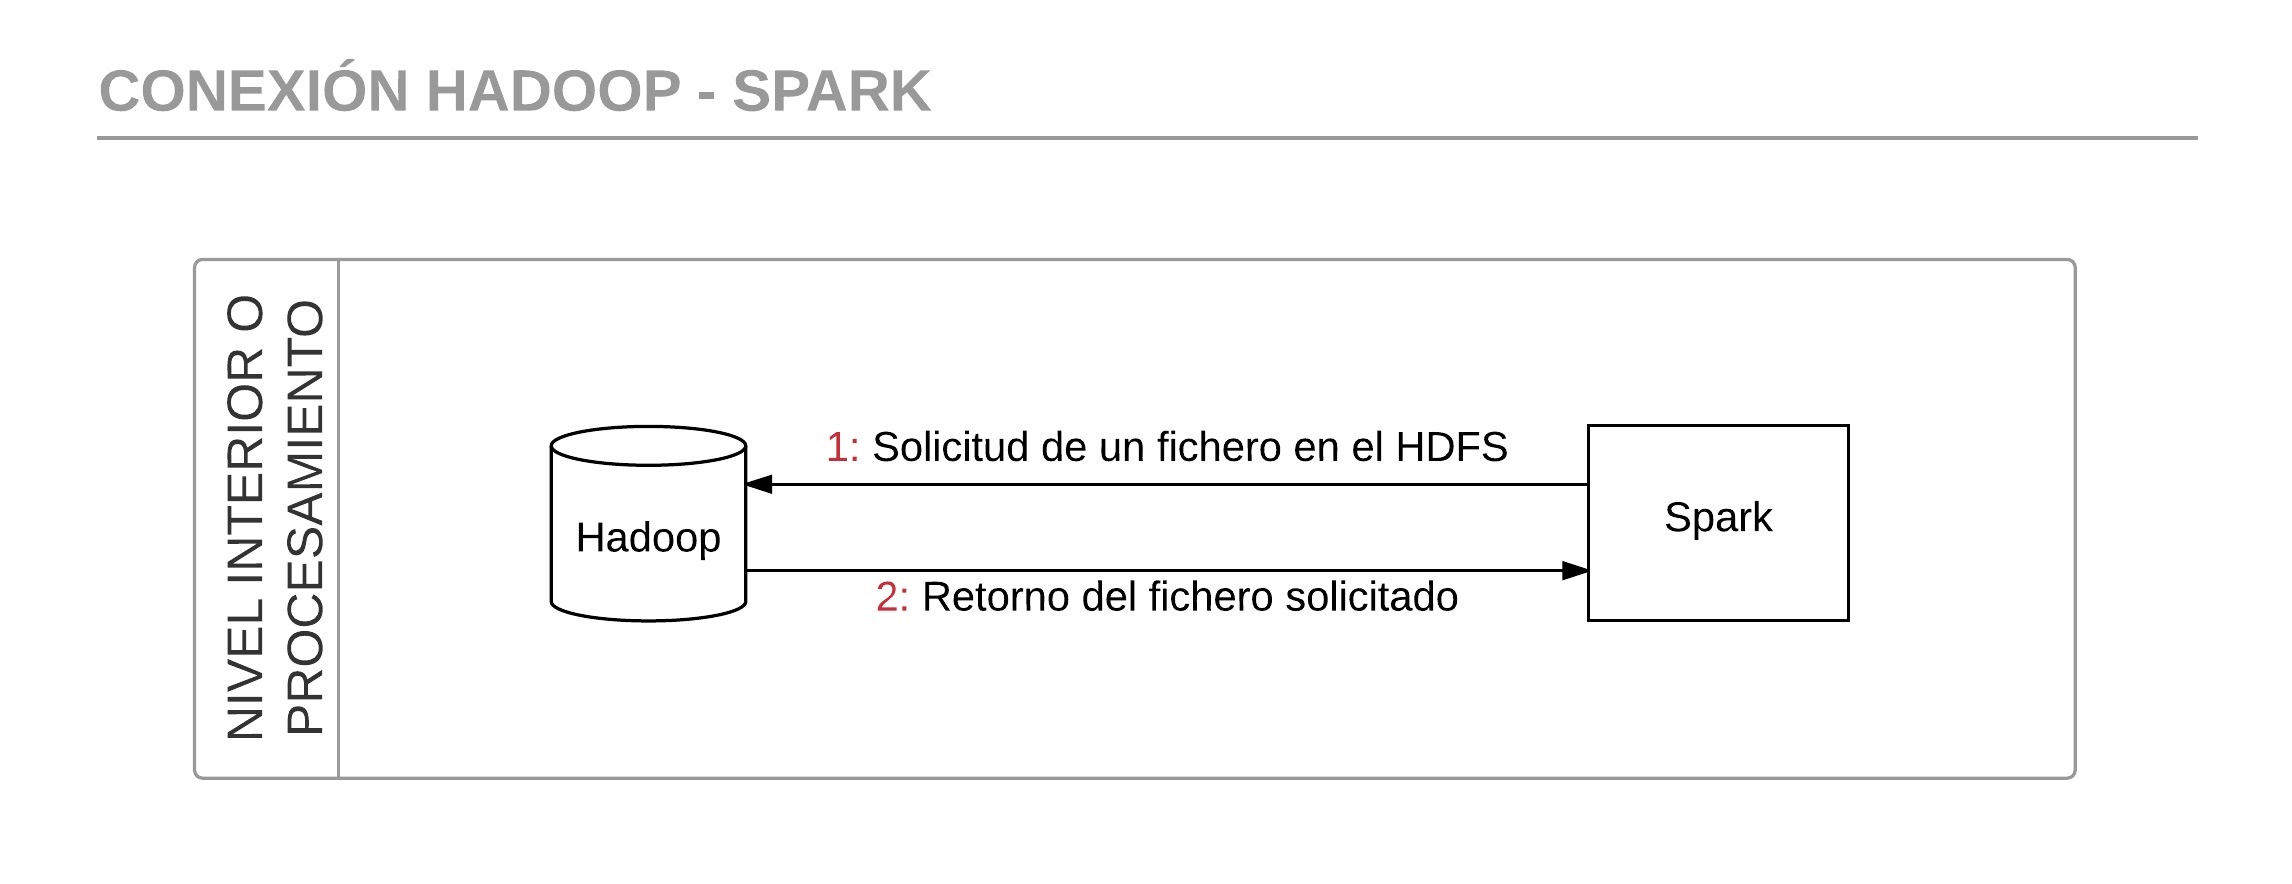
\includegraphics[width=1\linewidth]{imagenes/Conexion_Hadoop_Spark}
	\caption{Representación gráfica de la conexión Hadoop - Spark}
	\label{fig:conexionhadoopspark}
\end{figure}

\subsection{Spark - MongoDB}
Spark no trae integrada la conexión con MongoDB como ocurre en el caso de Hadoop. Para ello, la empresa de MongoDB provee una librería llamada ‘Mongo-Spark-Connector’ \cite{SparkMongoConexion}, que contiene las funciones necesarias para establecer comunicación entre estas dos herramientas. 

\begin{figure}
	\centering
	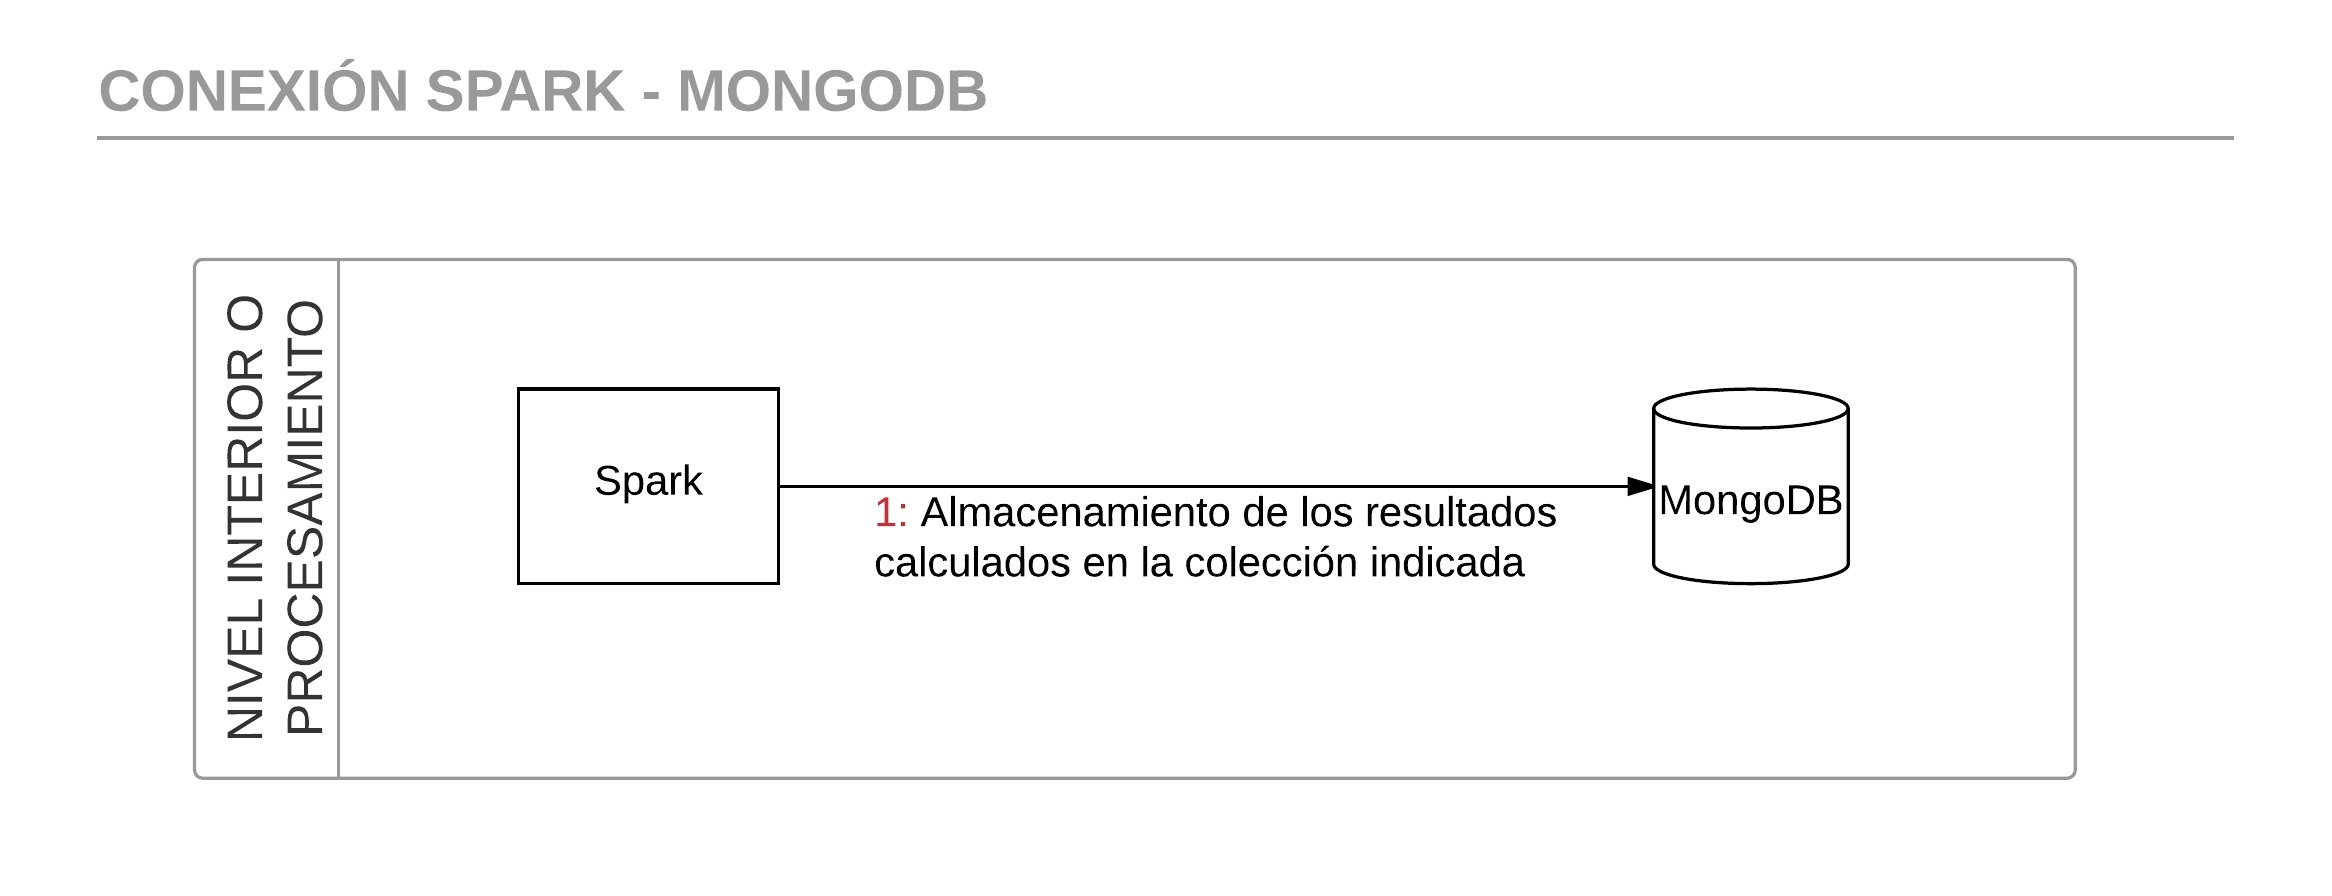
\includegraphics[width=1\linewidth]{imagenes/Conexion_Spark_MongoDB}
	\caption{Representación gráfica de la conexión Spark - MongoDB}
	\label{fig:conexionsparkmongodb}
\end{figure}

Conociendo la URL donde está mongo activo, la base de datos y la colección donde se quiere almacenar el resultado generado y el SparkContext, es suficiente para utilizar el método ‘WriteConfig’ que provee esta librería. Después, pasando el resultado a una estructura de secuencia de Spark y posteriormente a JSON, se guarda el mismo utilizando la función ‘save’ de ‘MongoSpark’. Con esto, ya estaría el resultado en MongoDB a través de Spark. En la figura \ref{fig:conexionsparkmongodb} se aprecia el flujo de almacenamiento de los datos resultados.

\subsection{NodeJS - Hadoop}
Para obtener el listado de los ficheros y directorios dentro de una URL específica, la mejor forma es utilizar la API RESTful \cite{HadoopRestful} que proporciona Hadoop. Para ello es necesario utilizar la librería ‘Request’ de NodeJS, que permite realizar peticiones de tipo ‘get’ o ‘post’ a una URL de una web, pudiendo guardar el resultado en una variable. Solamente indicando la dirección y el puerto que da Hadoop para la API RESTful, indicándole la ruta donde se encuentra el archivo dentro del HDFS, y la opción ‘?op=LISTSTATUS’, se obtiene el resultado de una manera muy rápida, como se muestra en la figura \ref{fig:conexionnodejshadoop}. En este caso, en vez de guardarla, se redirecciona a la interfaz web para poder visualizarla. Después se le da formato en la interfaz con funciones Javascript.

\begin{figure}
	\centering
	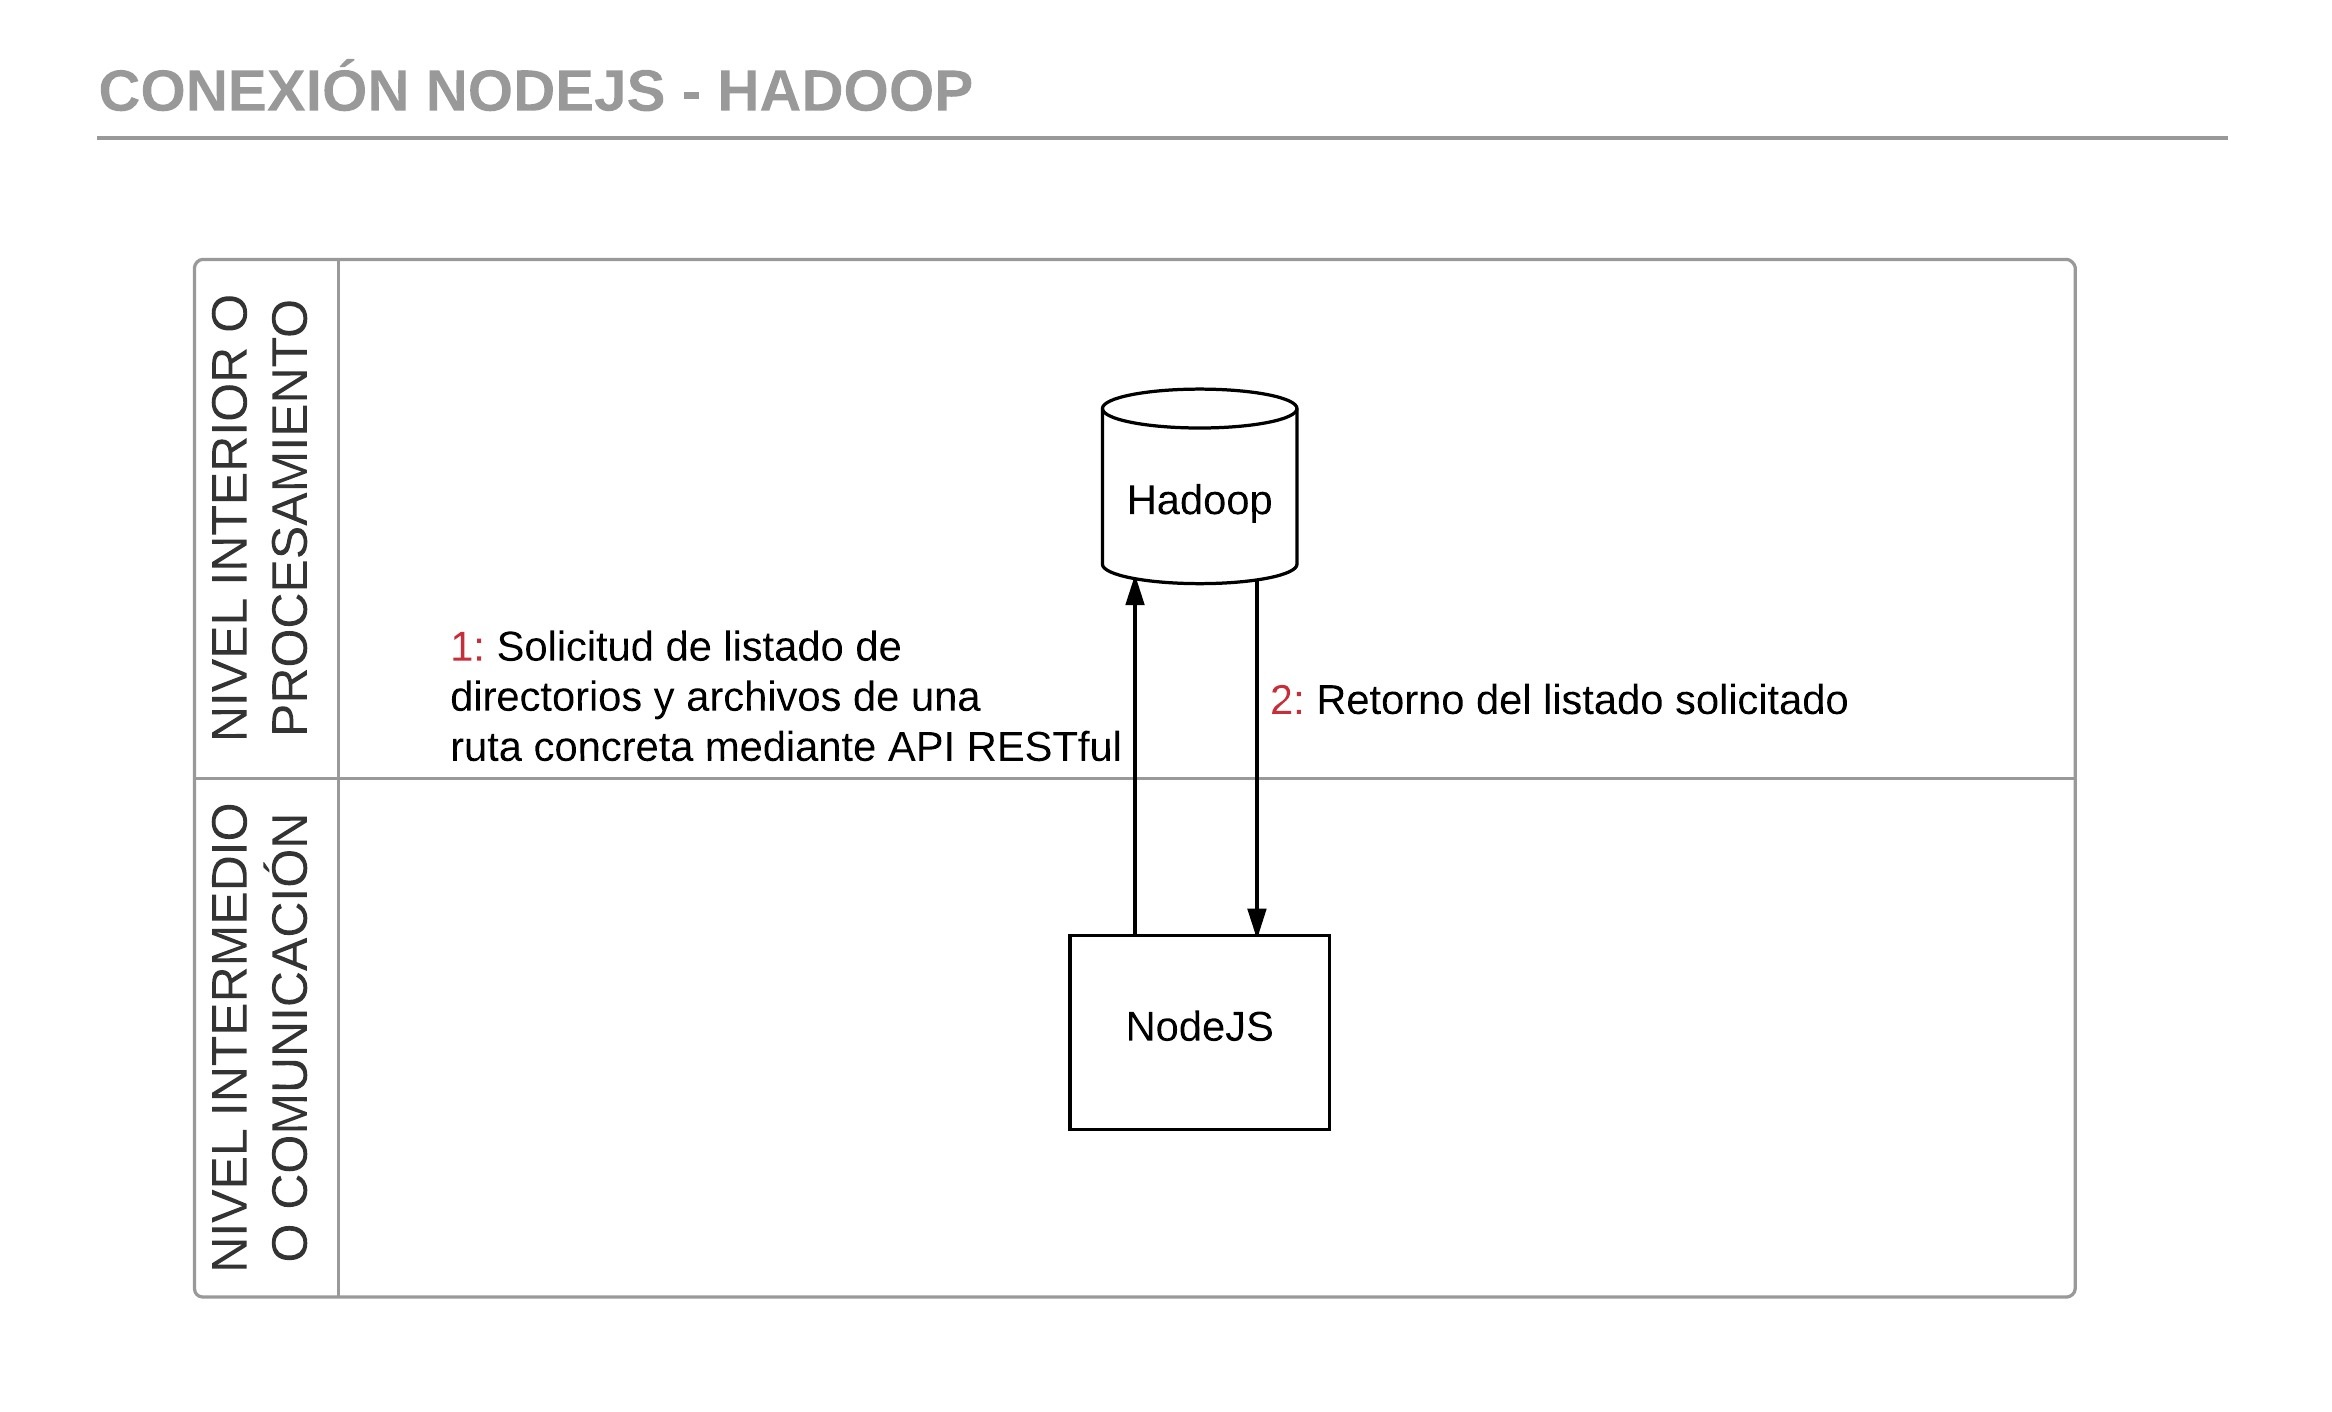
\includegraphics[width=1\linewidth]{imagenes/Conexion_NodeJS_Hadoop}
	\caption{Representación gráfica de la conexión NodeJS - Hadoop}
	\label{fig:conexionnodejshadoop}
\end{figure}


\subsection{NodeJS - Spark}

Existen varias formas de llamar a Spark desde NodeJS. Se puede lanzar un ejecutable a partir de la API RESTful que provee Spark, o lanzar el mismo ejecutable como si se lanzara desde un terminal, a través del comando ‘spark-submit’. Esta segunda opción ha sido la elegida, aunque se ha dejado como un desarrollo futuro la primera, ya que proporciona más información acerca de la ejecución de los códigos creados en Scala. 

\begin{figure}
	\centering
	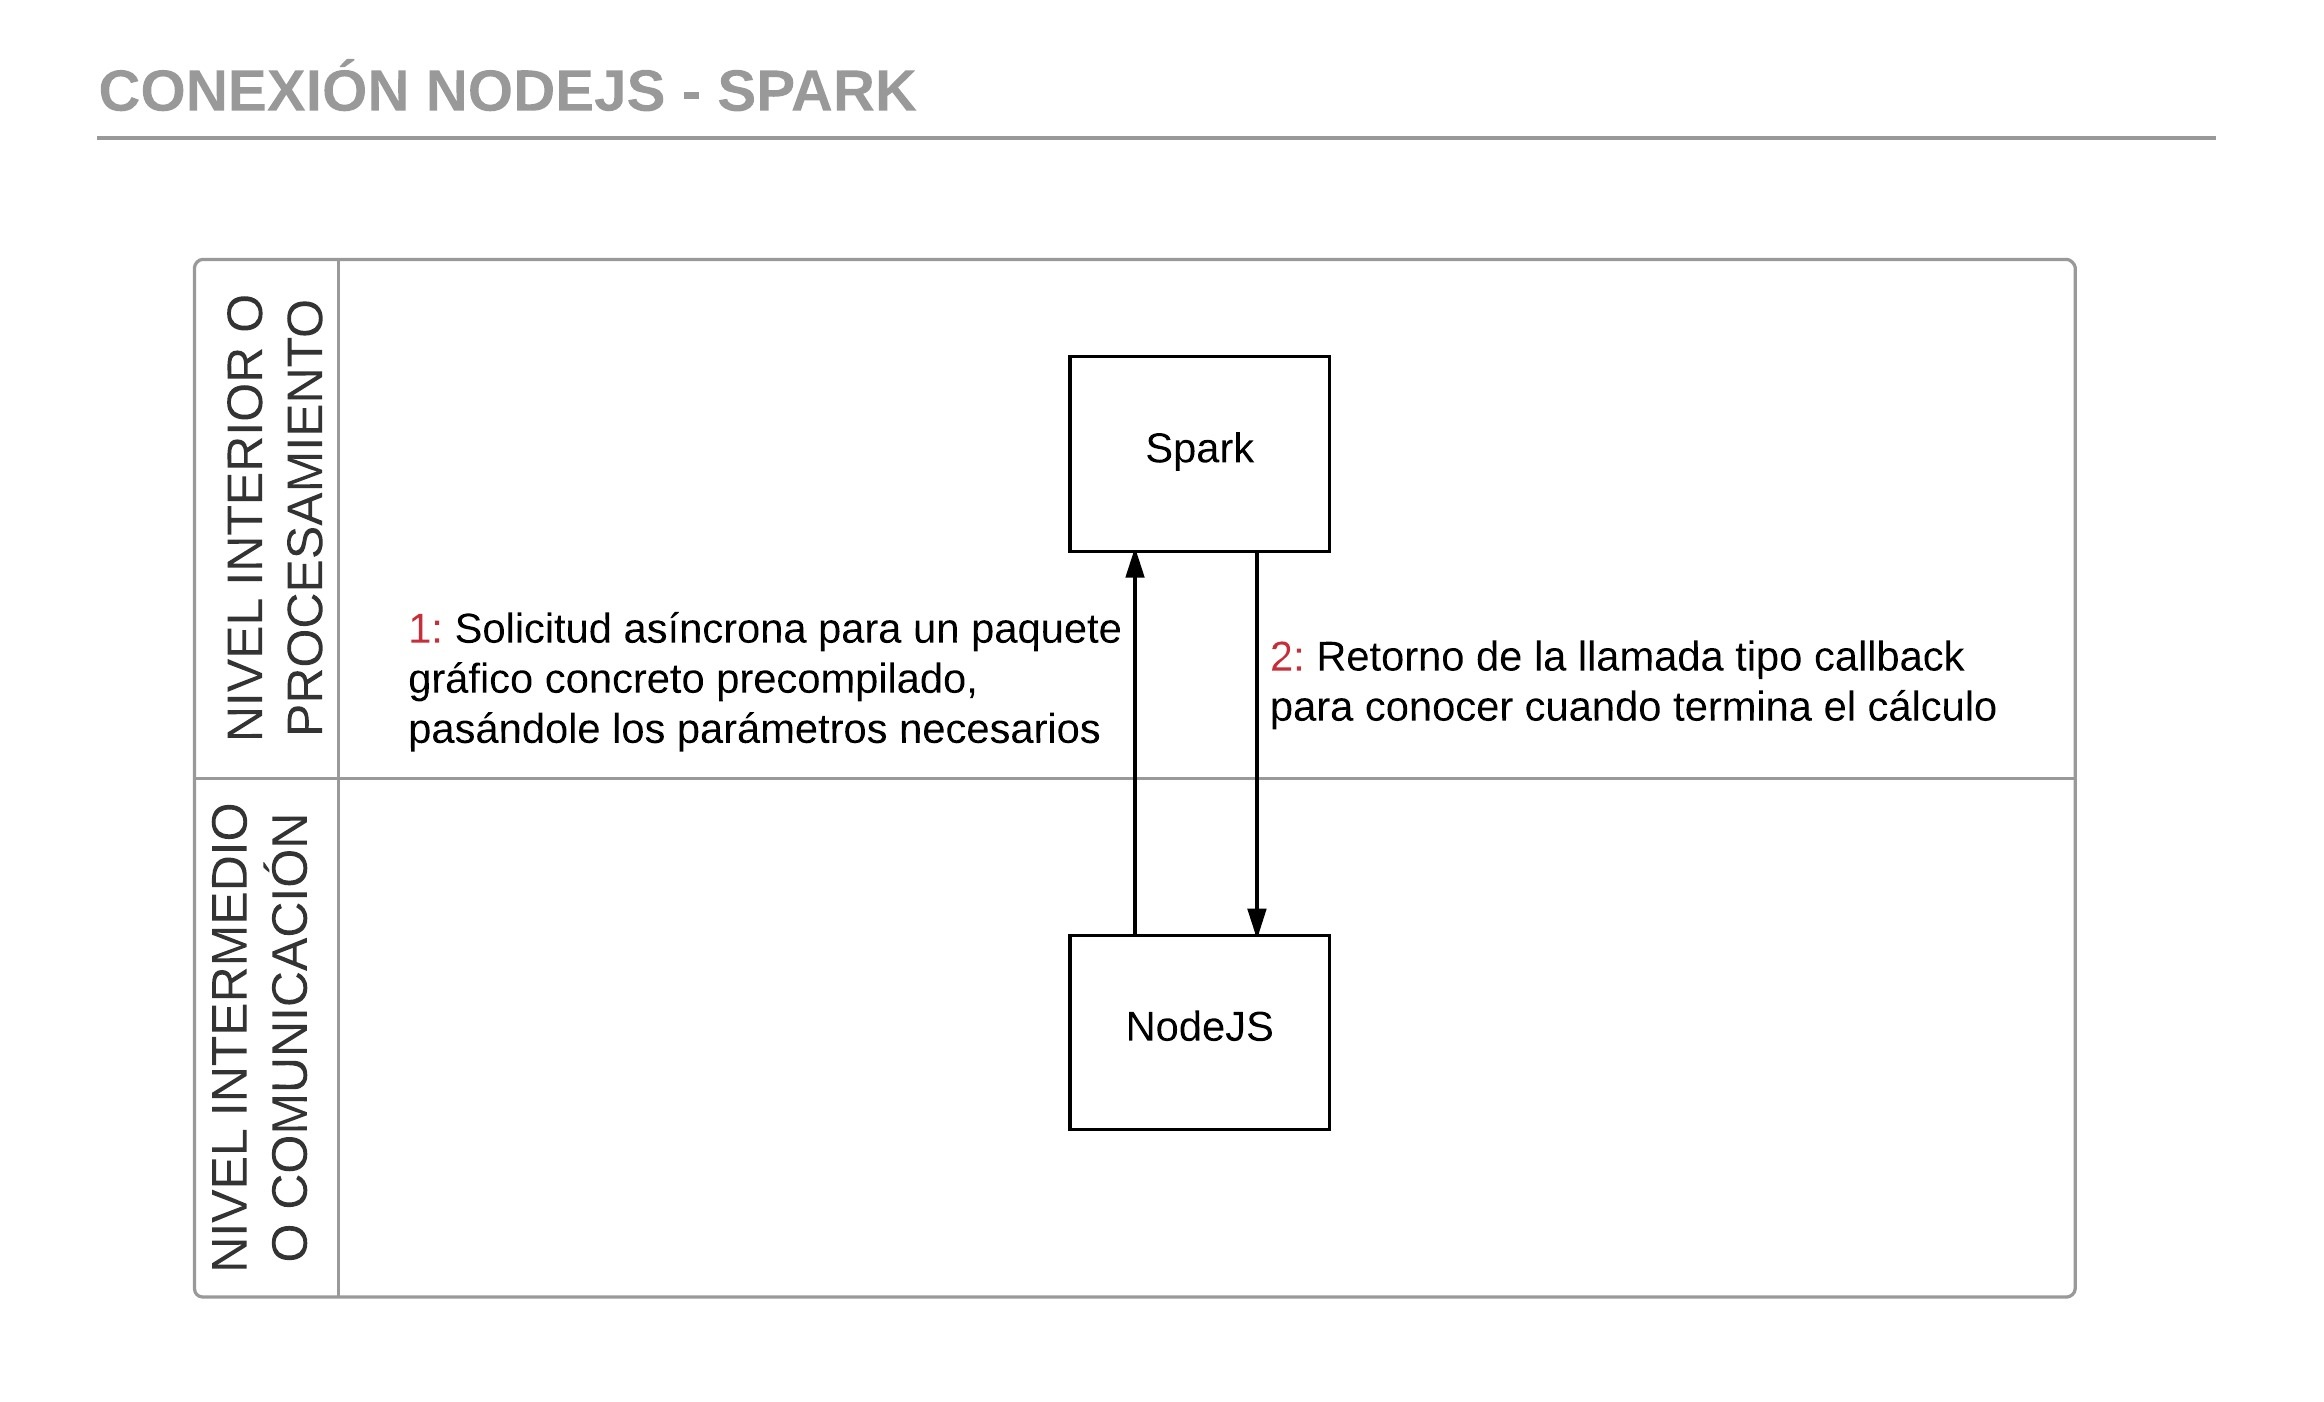
\includegraphics[width=1\linewidth]{imagenes/Conexion_NodeJS_Spark}
	\caption{Representación gráfica de la conexión NodeJS - Spark}
	\label{fig:conexionnodejsspark}
\end{figure}

Teniendo en cuenta esto, es necesario utilizar una librería diseñada para NodeJS llamada ‘node-cmd’ \cite{NodeCmd}, que permite ejecutar comandos como si de un terminal Linux se tratase. Se puede instalar desde el gestor NPM. Además, una de las grandes ventajas es que se puede ejecutar líneas de comandos de manera asíncrona y obtener la salida del mismo en formato String, para almacenarla en una variable si se necesitase. Tiene implementadas dos funciones, ‘run’ que ejecuta el comando y listo, o la función ‘get’, que además se puede indicar una función de tipo ‘callback’ para realizar alguna acción cuando termine la ejecución. En el sistema se ha utilizado la segunda, ya que proporciona más información para seguir trabajando después de la ejecución. 

Cuando se solicite un nuevo gráfico a través de la interfaz web, NodeJS recogerá la información y la pasará al comando ‘spark-submit’ junto con otros datos como la dirección del archivo en el HDFS o la dirección de MongoDB con el nombre de la base de datos y la colección para guardar el resultado. Se puede apreciar el flujo de llamadas en la figura \ref{fig:conexionnodejsspark}

\subsection{NodeJS - MongoDB}

Como ocurre con la conexión con Spark, NodeJS tampoco contiene funcionalidad para conectar con una base de datos en MongoDB. \textbf{Mongoose} \cite{MongooseInicial} es la librería que implementa las herramientas necesarias para lograr este objetivo. Trae consigo mucha funcionalidad para gestionar las bases de datos y las colecciones del sistema MongoDB que esté instalado en el ordenador o cluster. Haciendo una conexión muy sencilla con la función ‘createConnection’, indicándole solamente la URL donde se encuentra la base de datos y la colección, entonces se podrá obtener los documentos en formato JSON que se encuentran alojados en la misma, teniendo la posibilidad de realizar filtros o selecciones concretas sobre los datos. Con esta función se pueden realizar varios accesos de manera concurrente a la base de datos, gestionando ella misma la exclusión mutua. En la figura \ref{fig:conexionnodejsmongodb} se puede ver la conexión entre las herramientas en distintos niveles.

\begin{figure}
	\centering
	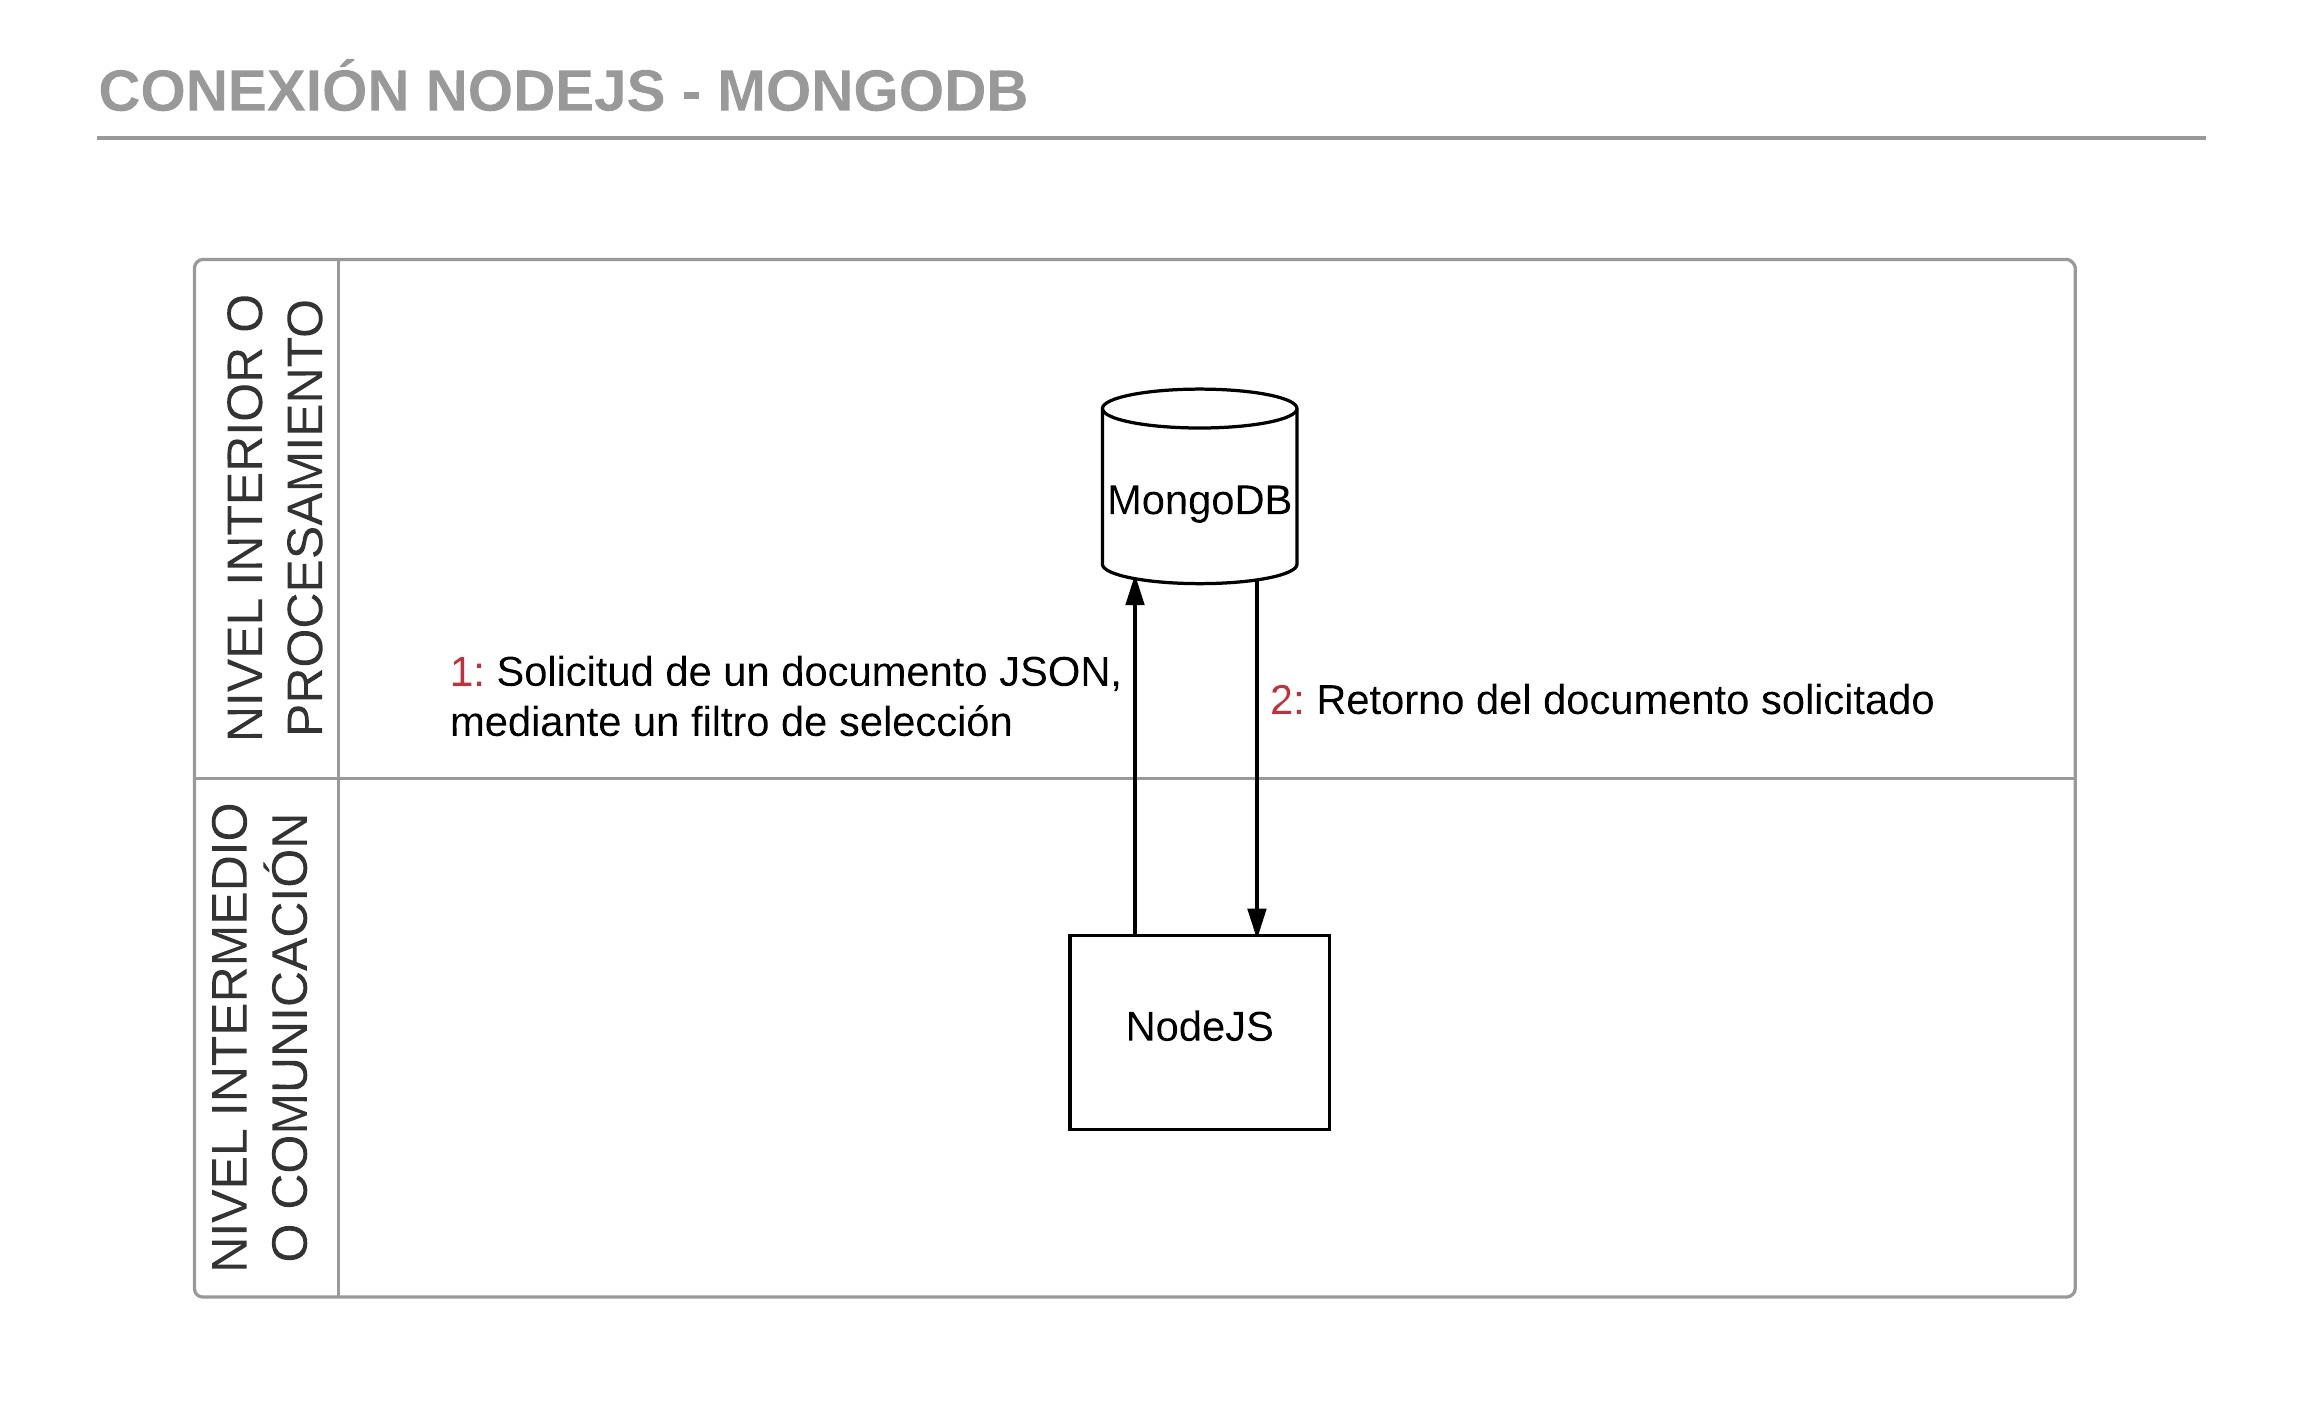
\includegraphics[width=1\linewidth]{imagenes/Conexion_NodeJS_MongoDB}
	\caption{Representación gráfica de la conexión NodeJS - MongoDB}
	\label{fig:conexionnodejsmongodb}
\end{figure}

En el sistema, se utiliza para dos cosas. La primera es para insertar y modificar los documentos que mantienen el estado de una ejecución, dentro de una colección habilitada para ello. Ahí se almacena el identificador de la ejecución, el estado en el que se encuentra y las fechas de inicio y fin. La segunda es para buscar el resultado que ha dejado Spark en la colección de la base de datos específica, filtrando los datos por el identificador que se generó previamente.

\subsection{NodeJS - D3JS}

D3JS es una librería muy potente que permite generar desde sencillos gráficos hasta de los más complejos, dándole incluso dinamismo. En NodeJS se puede integrar a través del gestor de paquetes NPM, para poder acceder a la amplia gama de funciones para generar los infogramas. La propia librería provee una galería de gráficos de ejemplo \cite{D3JSGallery} para ayudar a implementar cualquiera. Al ser totalmente abierta, el desarrollador es libre de modificar cualquiera de estos ejemplos a sus propias necesidades, o incluso diseñar uno desde cero.

Dentro de esta galería, se han utilizado uno o varios ejemplos para la creación del listado de gráficos disponibles en la API, adaptándolos a los datos resultados. Ya que no es viable generar un gráfico con todos los datos que puede contener dentro del concepto de ‘Big Data’, por eso son necesarias las técnicas de reducción y agrupación de las que se encarga Spark, teniendo en cuenta que los resultados que se dibujen en la gráfica sean representativos de lo que ocurre con los datos. 

Cabe destacar que forma parte de la propia experiencia del usuario de la API, seleccionar el gráfico adecuado para los datos seleccionados

\subsection{Interfaz web - NodeJS}

La conexión de NodeJS con la interfaz web, sigue una estructura de cliente-servidor. Es el propio usuario el que solicita información a través de la web al servidor, el cual debe retornar lo solicitado dentro de un tiempo razonable. NodeJS implementa una conexión nativa con las aplicaciones web, permitiendo la comunicación entre ambas partes, como se puede ver en la figura \ref{fig:conexioninterfaznodejs}.

\begin{figure}
	\centering
	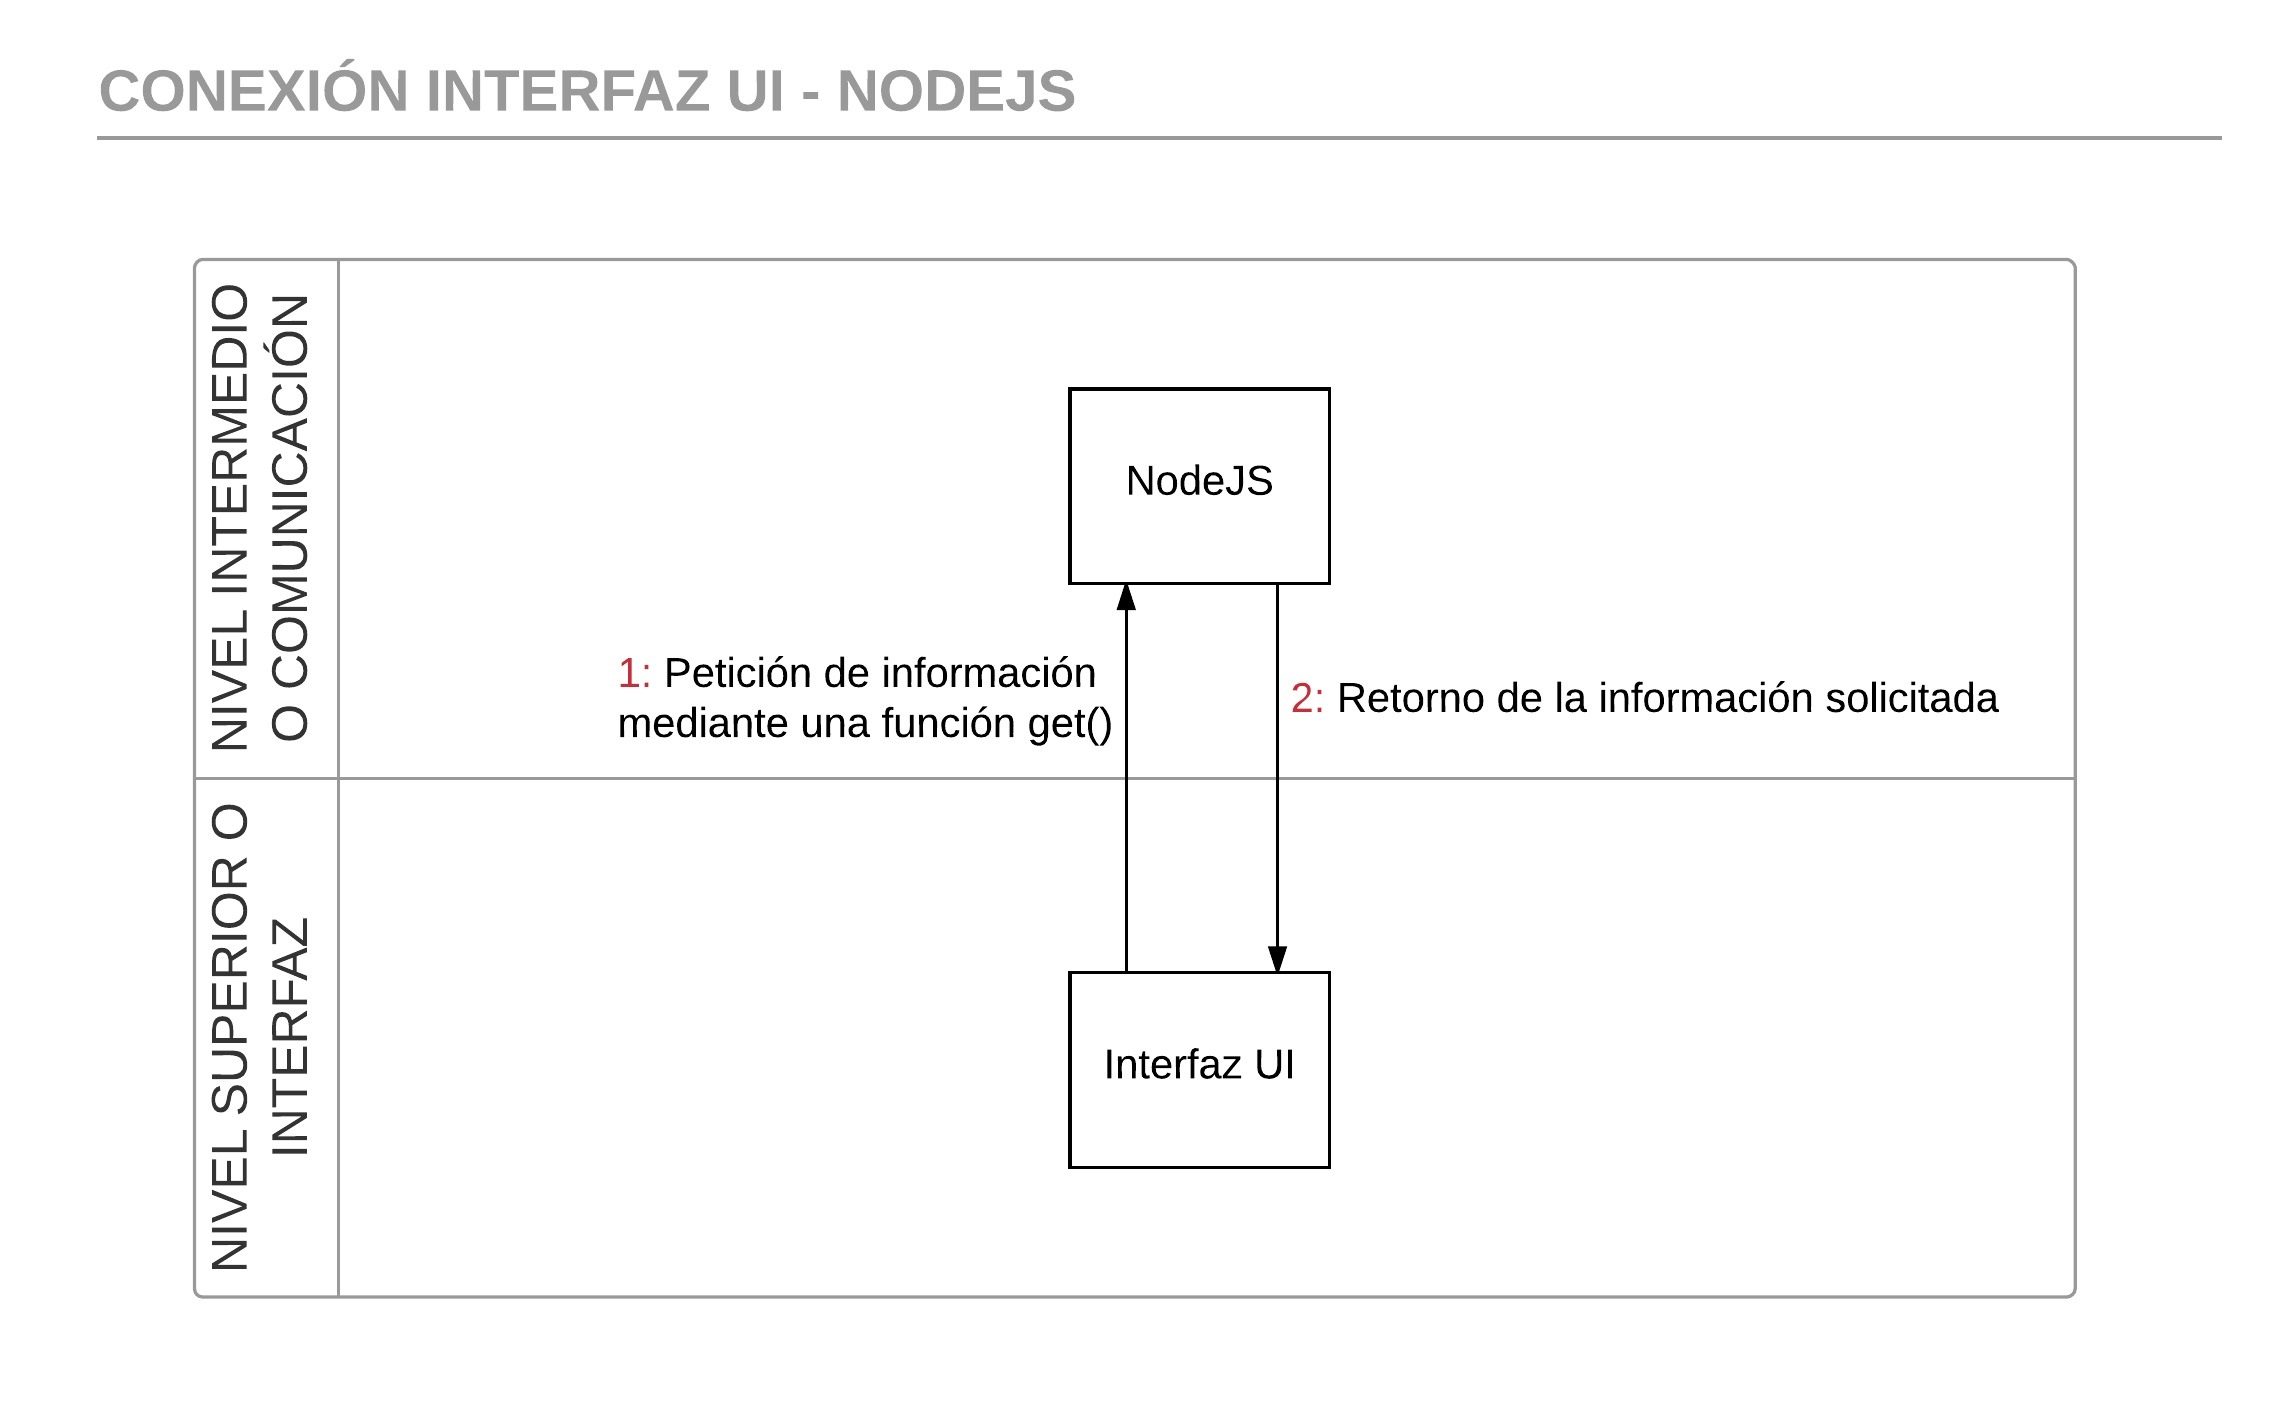
\includegraphics[width=1\linewidth]{imagenes/Conexion_Interfaz_NodeJS}
	\caption{Representación gráfica de la conexión Interfaz web - NodeJS}
	\label{fig:conexioninterfaznodejs}
\end{figure}

Además, NodeJS trae implementado un gestor de plantillas de tipo JADE (o PUG renombrado en las últimas versiones) \cite{PugInicial}. Pug es un motor de plantillas, diseñado para simplificar la escritura de código HTML, que está integrado en NodeJS. Con Pug se resume la cantidad de código que es necesario escribir para el diseño de una página HTML, siguiendo una estructura muy sencilla. NodeJS se encarga de traducir las plantillas escritas en Pug a código HTML, para que el navegador web pueda ejecutarlo. Cabe destacar que cuando se comenzó con este proyecto, todavía era Jade, dejando como tarea a desarrollar la actualización del contenido escrito en esta plantilla.

\section{Flujo de procesamiento}

En este apartado se va a explicar cómo funciona internamente el sistema cuando se solicita alguna de las funcionalidades disponibles desde la interfaz web. Lo primero es listar las funciones que se pueden realizar y explicar cada una por separado. 

\subsection{Mostrar el listado de archivos y directorios en el HDFS}

Desde la interfaz, el usuario solicita, o el propio sistema automáticamente al iniciar la API, a NodeJS listar el contenido de un directorio específico dentro del HDFS. En el caso del inicio del sistema, se solicita el directorio raíz. Después NodeJS es el encargado de pedir y recuperar esta información a Hadoop, para a continuación, devolverla a la interfaz, que será la encargada de darle el formato correcto. En la figura \ref{fig:listararchivosdelhdfs} se puede apreciar gráficamente el flujo de llamadas entre las herramientas.

Cabe destacar que el sistema solo trata actualmente con ficheros de tipo CSV y que no estén vacíos. Ampliar el número de tipos de ficheros permitidos es una de las principales mejoras de este sistema.

\begin{figure}
	\centering
	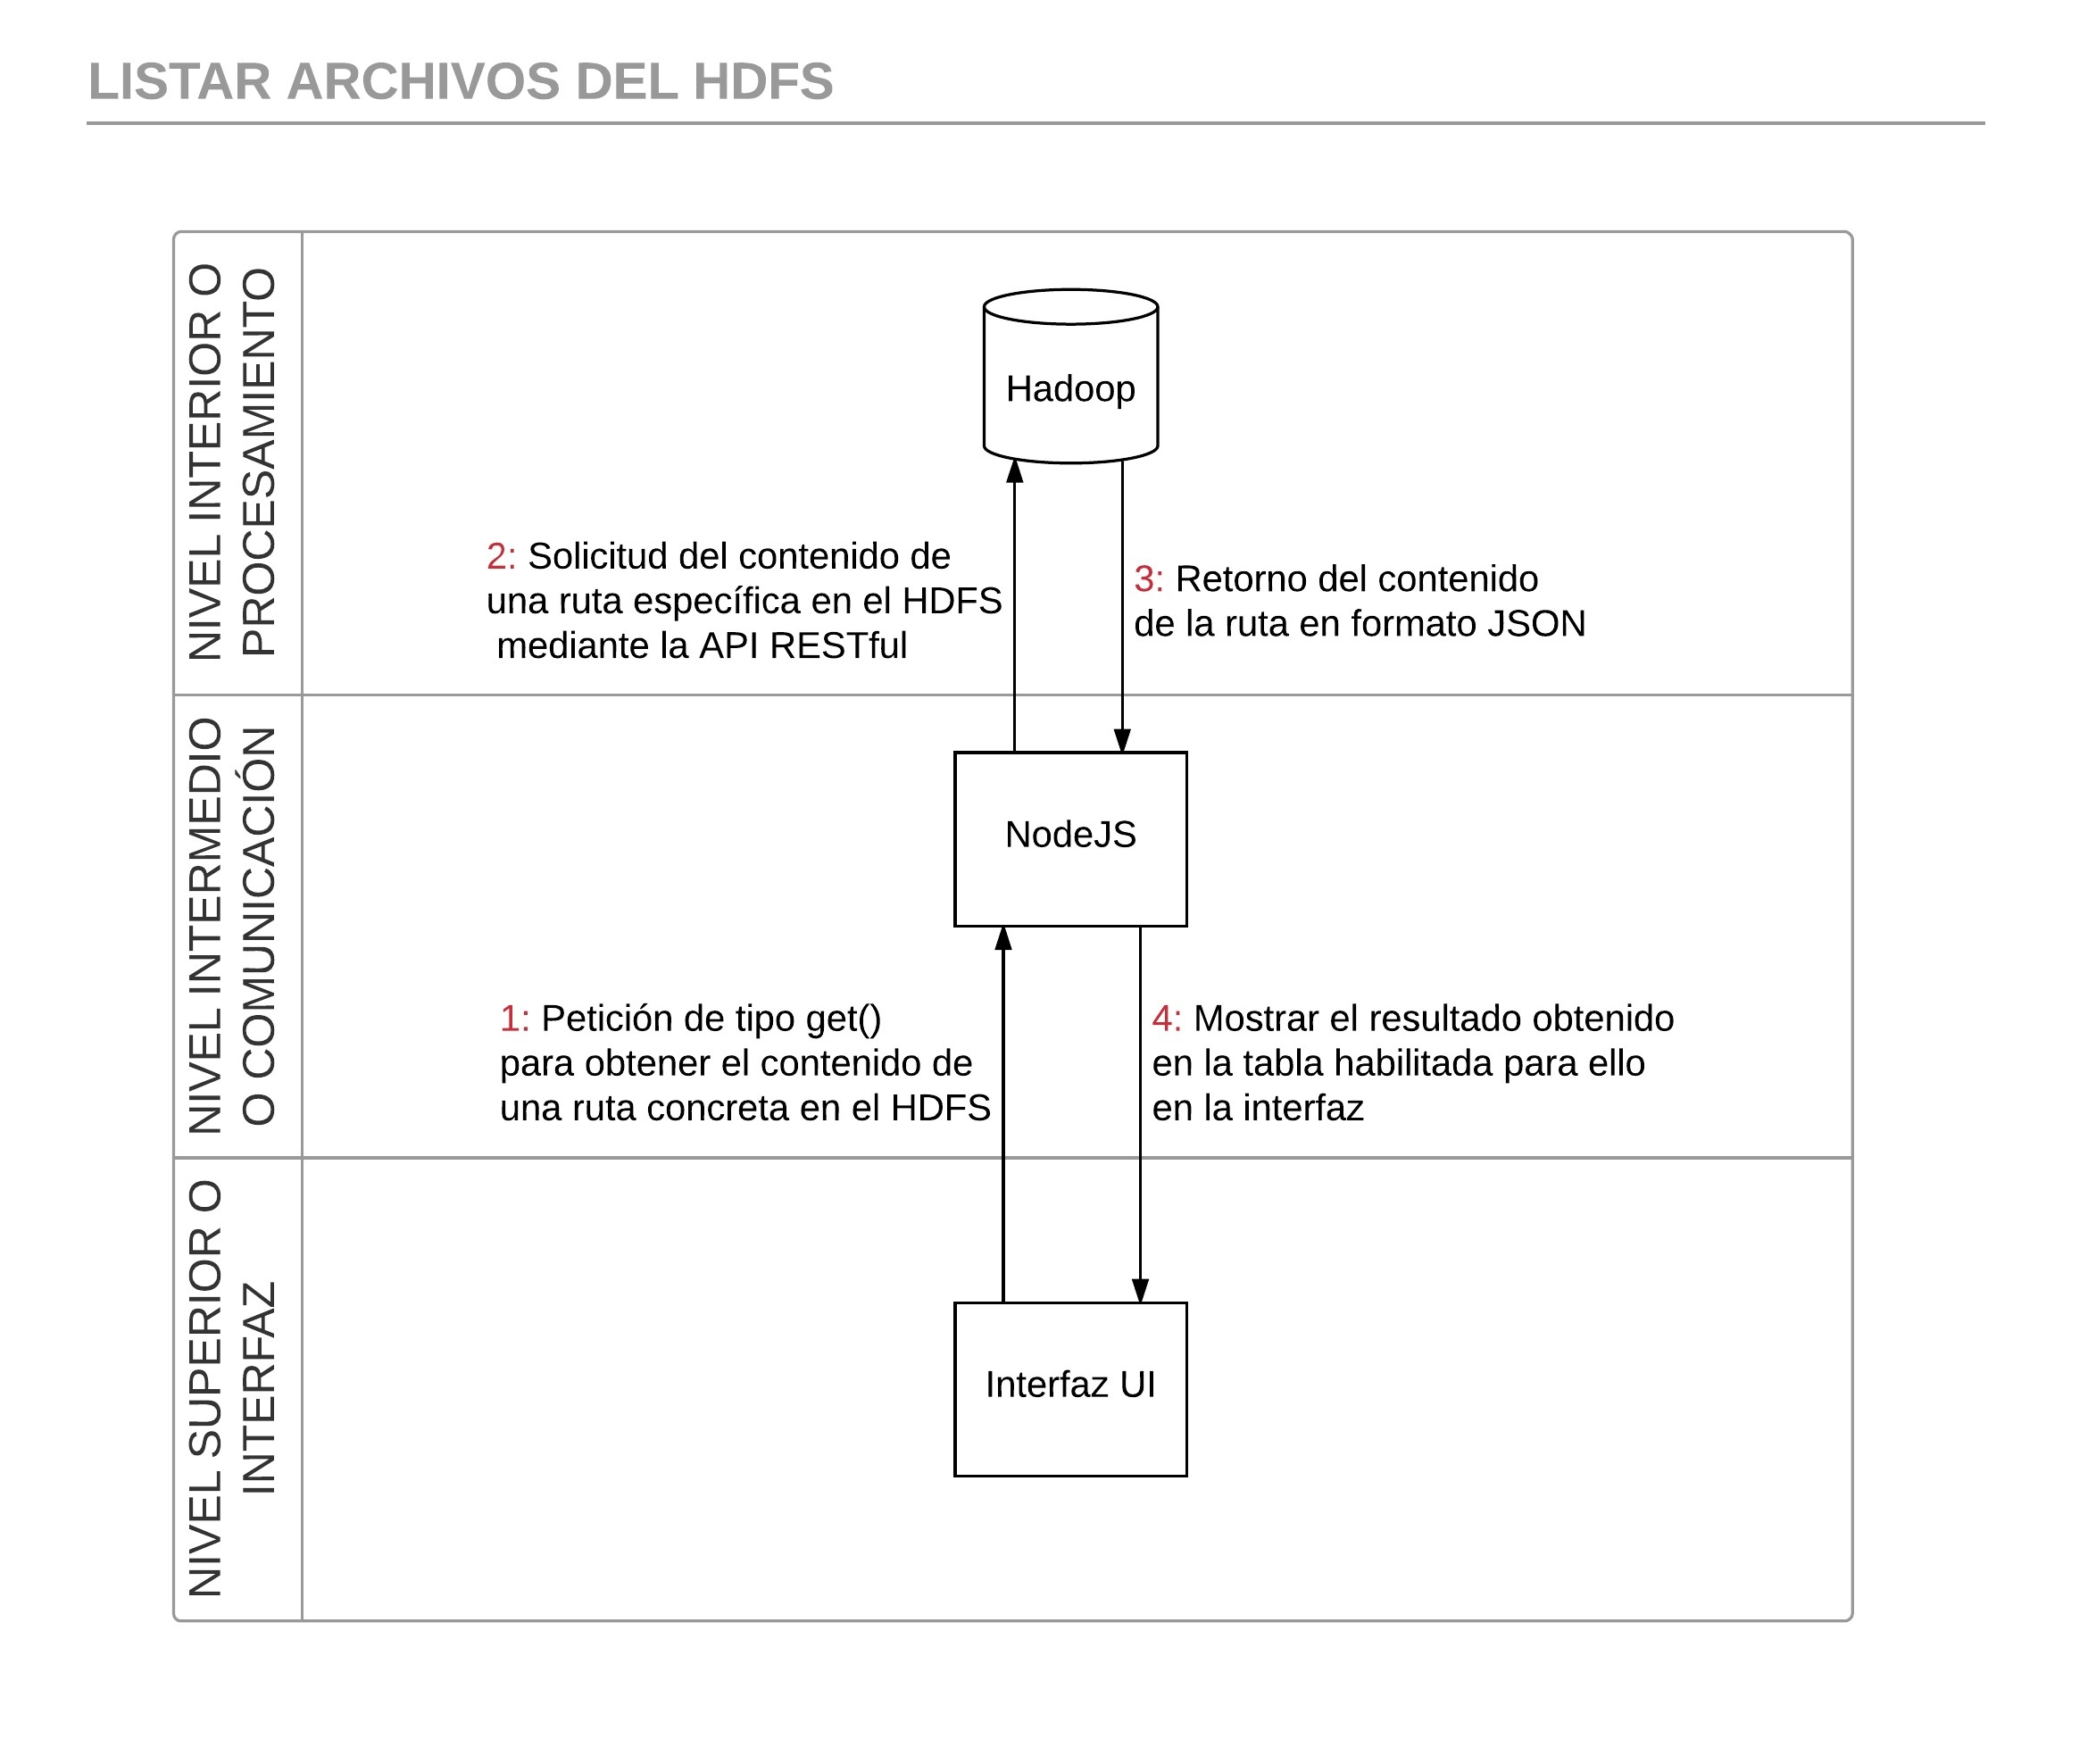
\includegraphics[width=1\linewidth]{imagenes/Listar_archivos_del_HDFS}
	\caption{Flujo de llamadas para listar el contenido del HDFS}
	\label{fig:listararchivosdelhdfs}
\end{figure}

\subsection{Ejecución de un proceso seleccionado}

Ya se trate de mostrar el resumen de un fichero seleccionado, solicitar un gráfico bajo unos parámetros concretos o simplemente mostrar los datos de dicho gráfico, el proceso que realiza el sistema internamente es el mismo. 

El primer paso es la solicitud de mostrar esa información por parte del usuario. Para ello, la interfaz web recoge los parámetros que necesita para ejecutar la función correspondiente. Si es para mostrar la información resumen del contenido de un fichero, basta con enviarle a NodeJS que fichero es y en que ruta está almacenado. En el caso que se quiera un gráfico o los datos resultados directamente, habrá que añadir todos los parámetros indicados en el formulario de la interfaz habilitado para cada uno de los infogramas disponibles. 

A continuación, NodeJS genera un identificador del proceso a partir de la ruta del fichero seleccionado, el tamaño del mismo, el gráfico que se desea generar y sus parámetros. Con el identificador creado, antes de realizar ninguna acción más, comprueba que el resultado del proceso no se encuentre ya en la colección, o esté calculándose paralelamente a este. En cuyo caso, el sistema se esperaría a que estuviese terminado para recuperar la información, evitando guardar resultados duplicados. Cuando terminase, devolverá el resultado a la interfaz para visualizarlo. Esta comprobación se explica gráficamente en la figura \ref{fig:procesoyaejecutadopreviamente}.

\begin{figure}
	\centering
	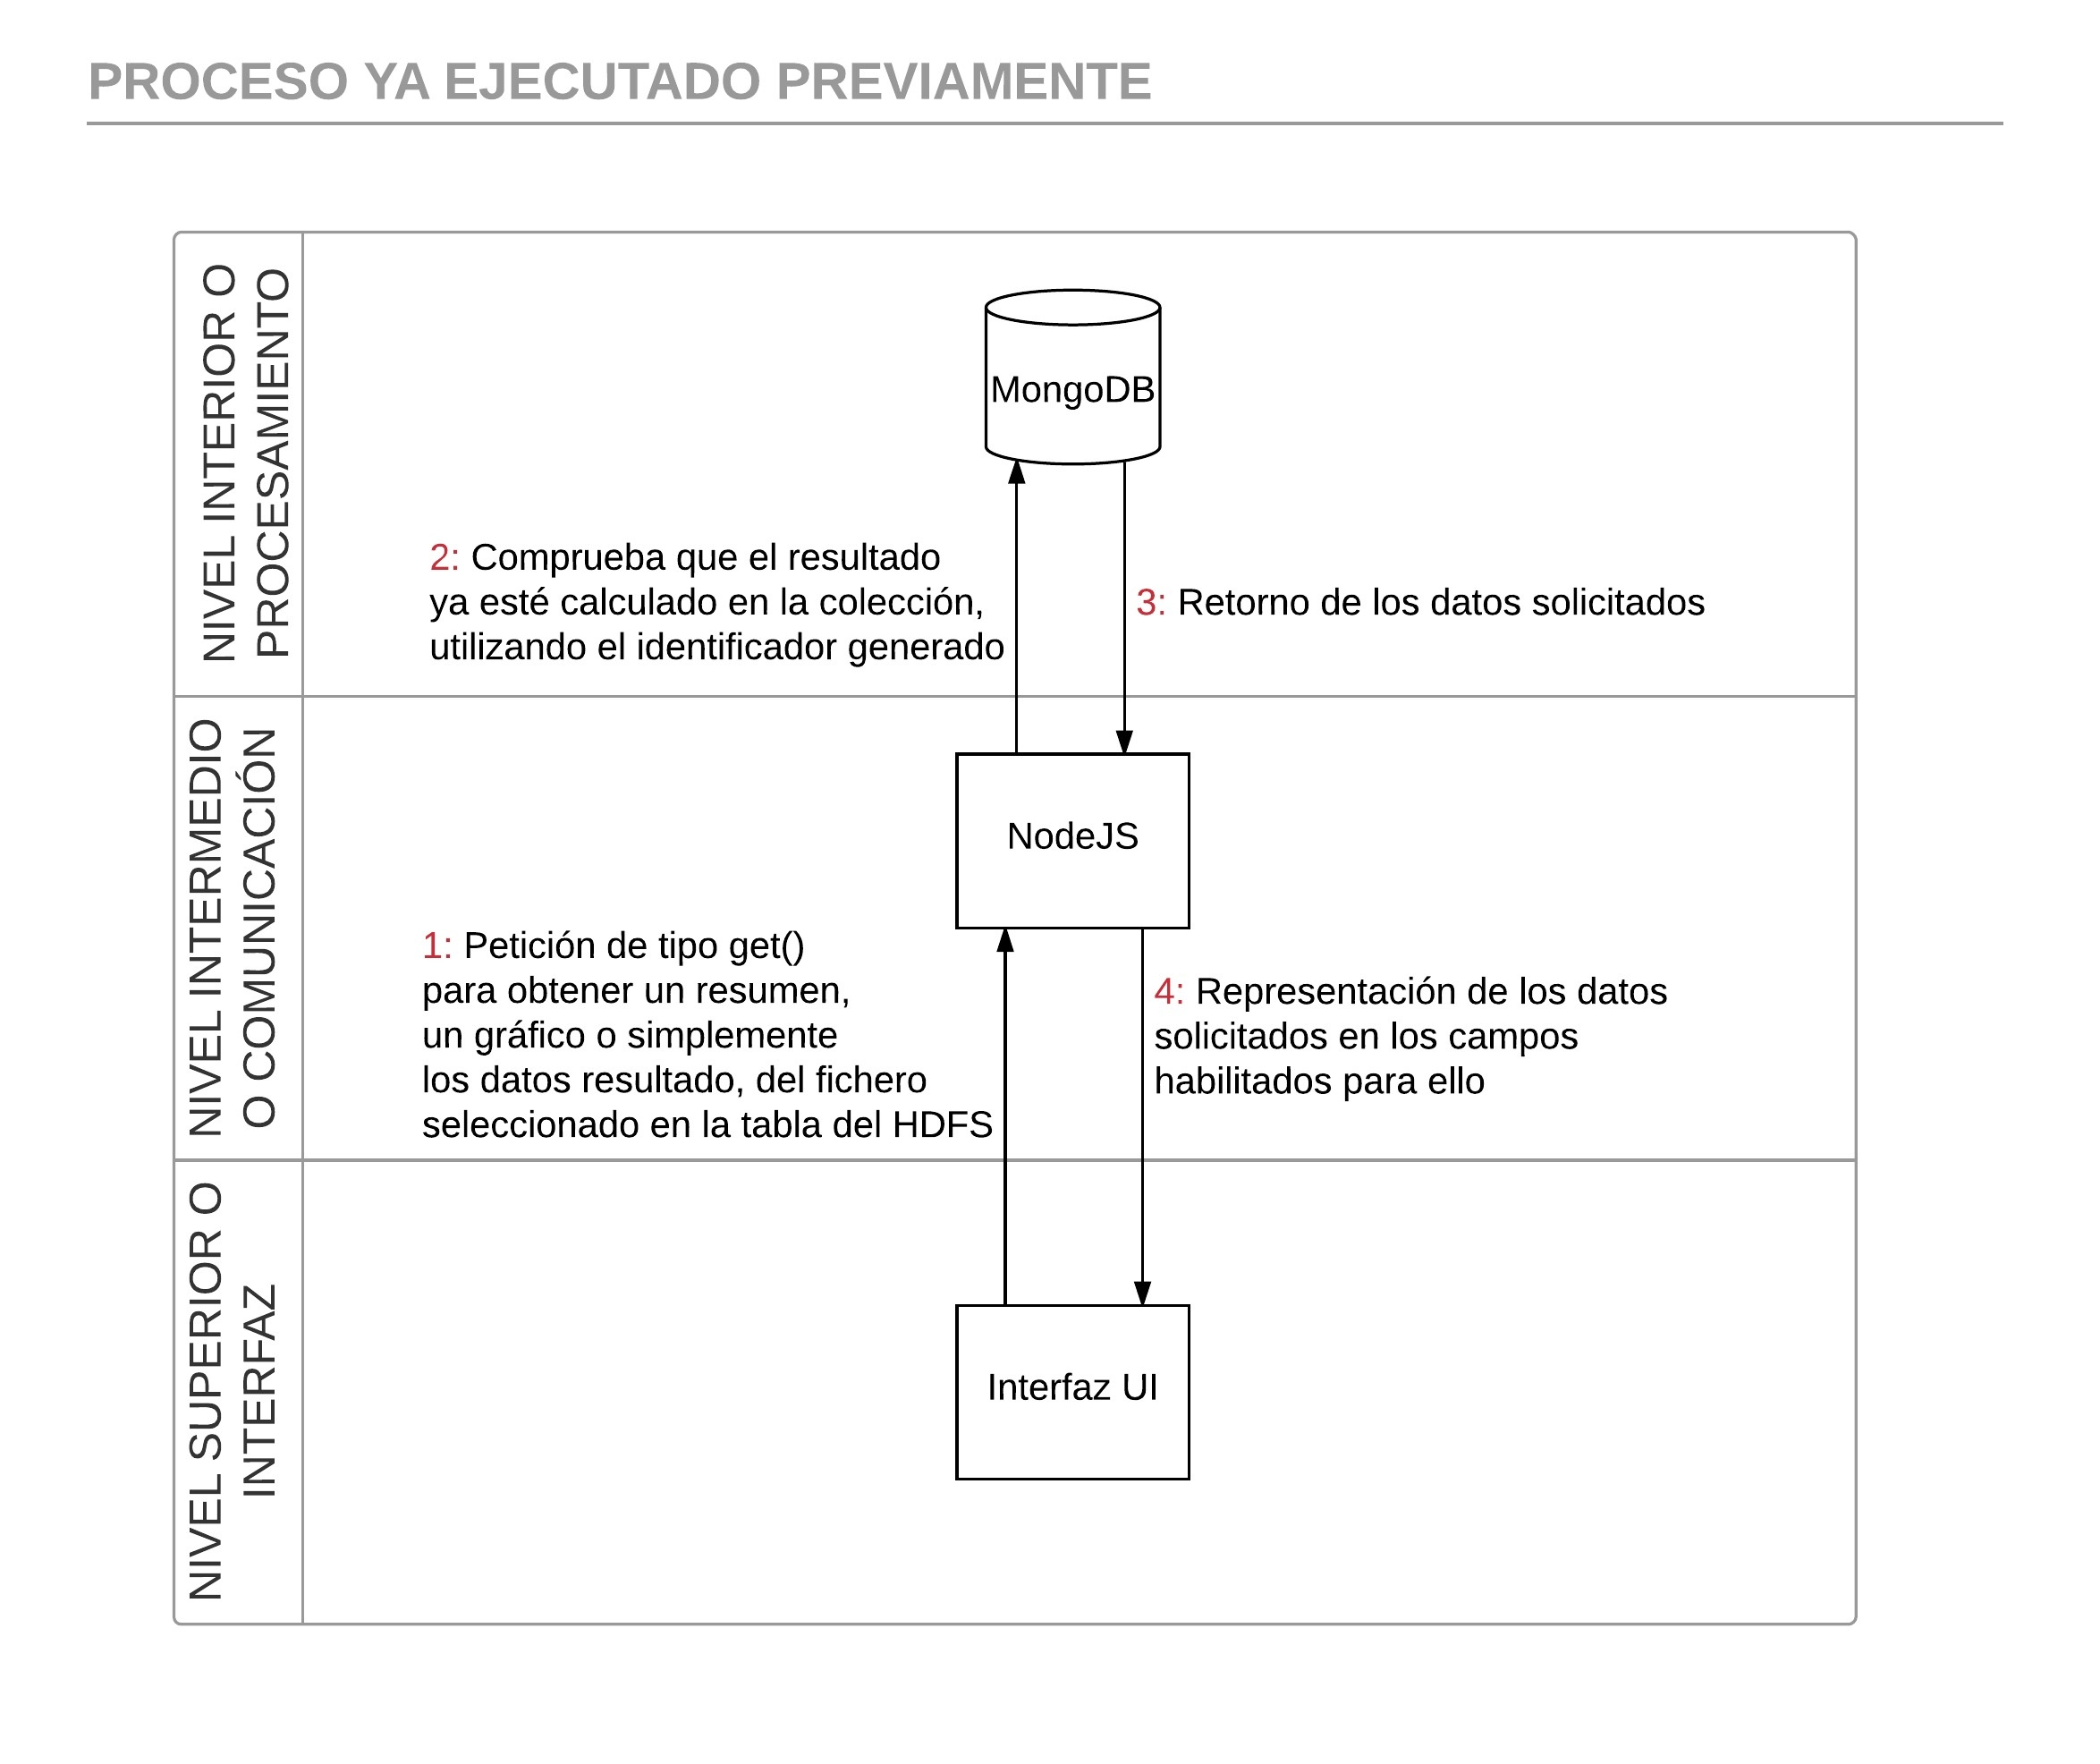
\includegraphics[width=1\linewidth]{imagenes/Proceso_ya_ejecutado_previamente}
	\caption{Ejecución de un proceso ya generado anteriormente}
	\label{fig:procesoyaejecutadopreviamente}
\end{figure}

Si no estuviera el resultado, tal y como se indica en la figura \ref{fig:ejecuciondeunproceso}, el siguiente paso sería generar un documento JSON con la información del estado actual del proceso y guardarlo en una colección habilitada para ello en MongoDB.

\begin{figure}
	\centering
	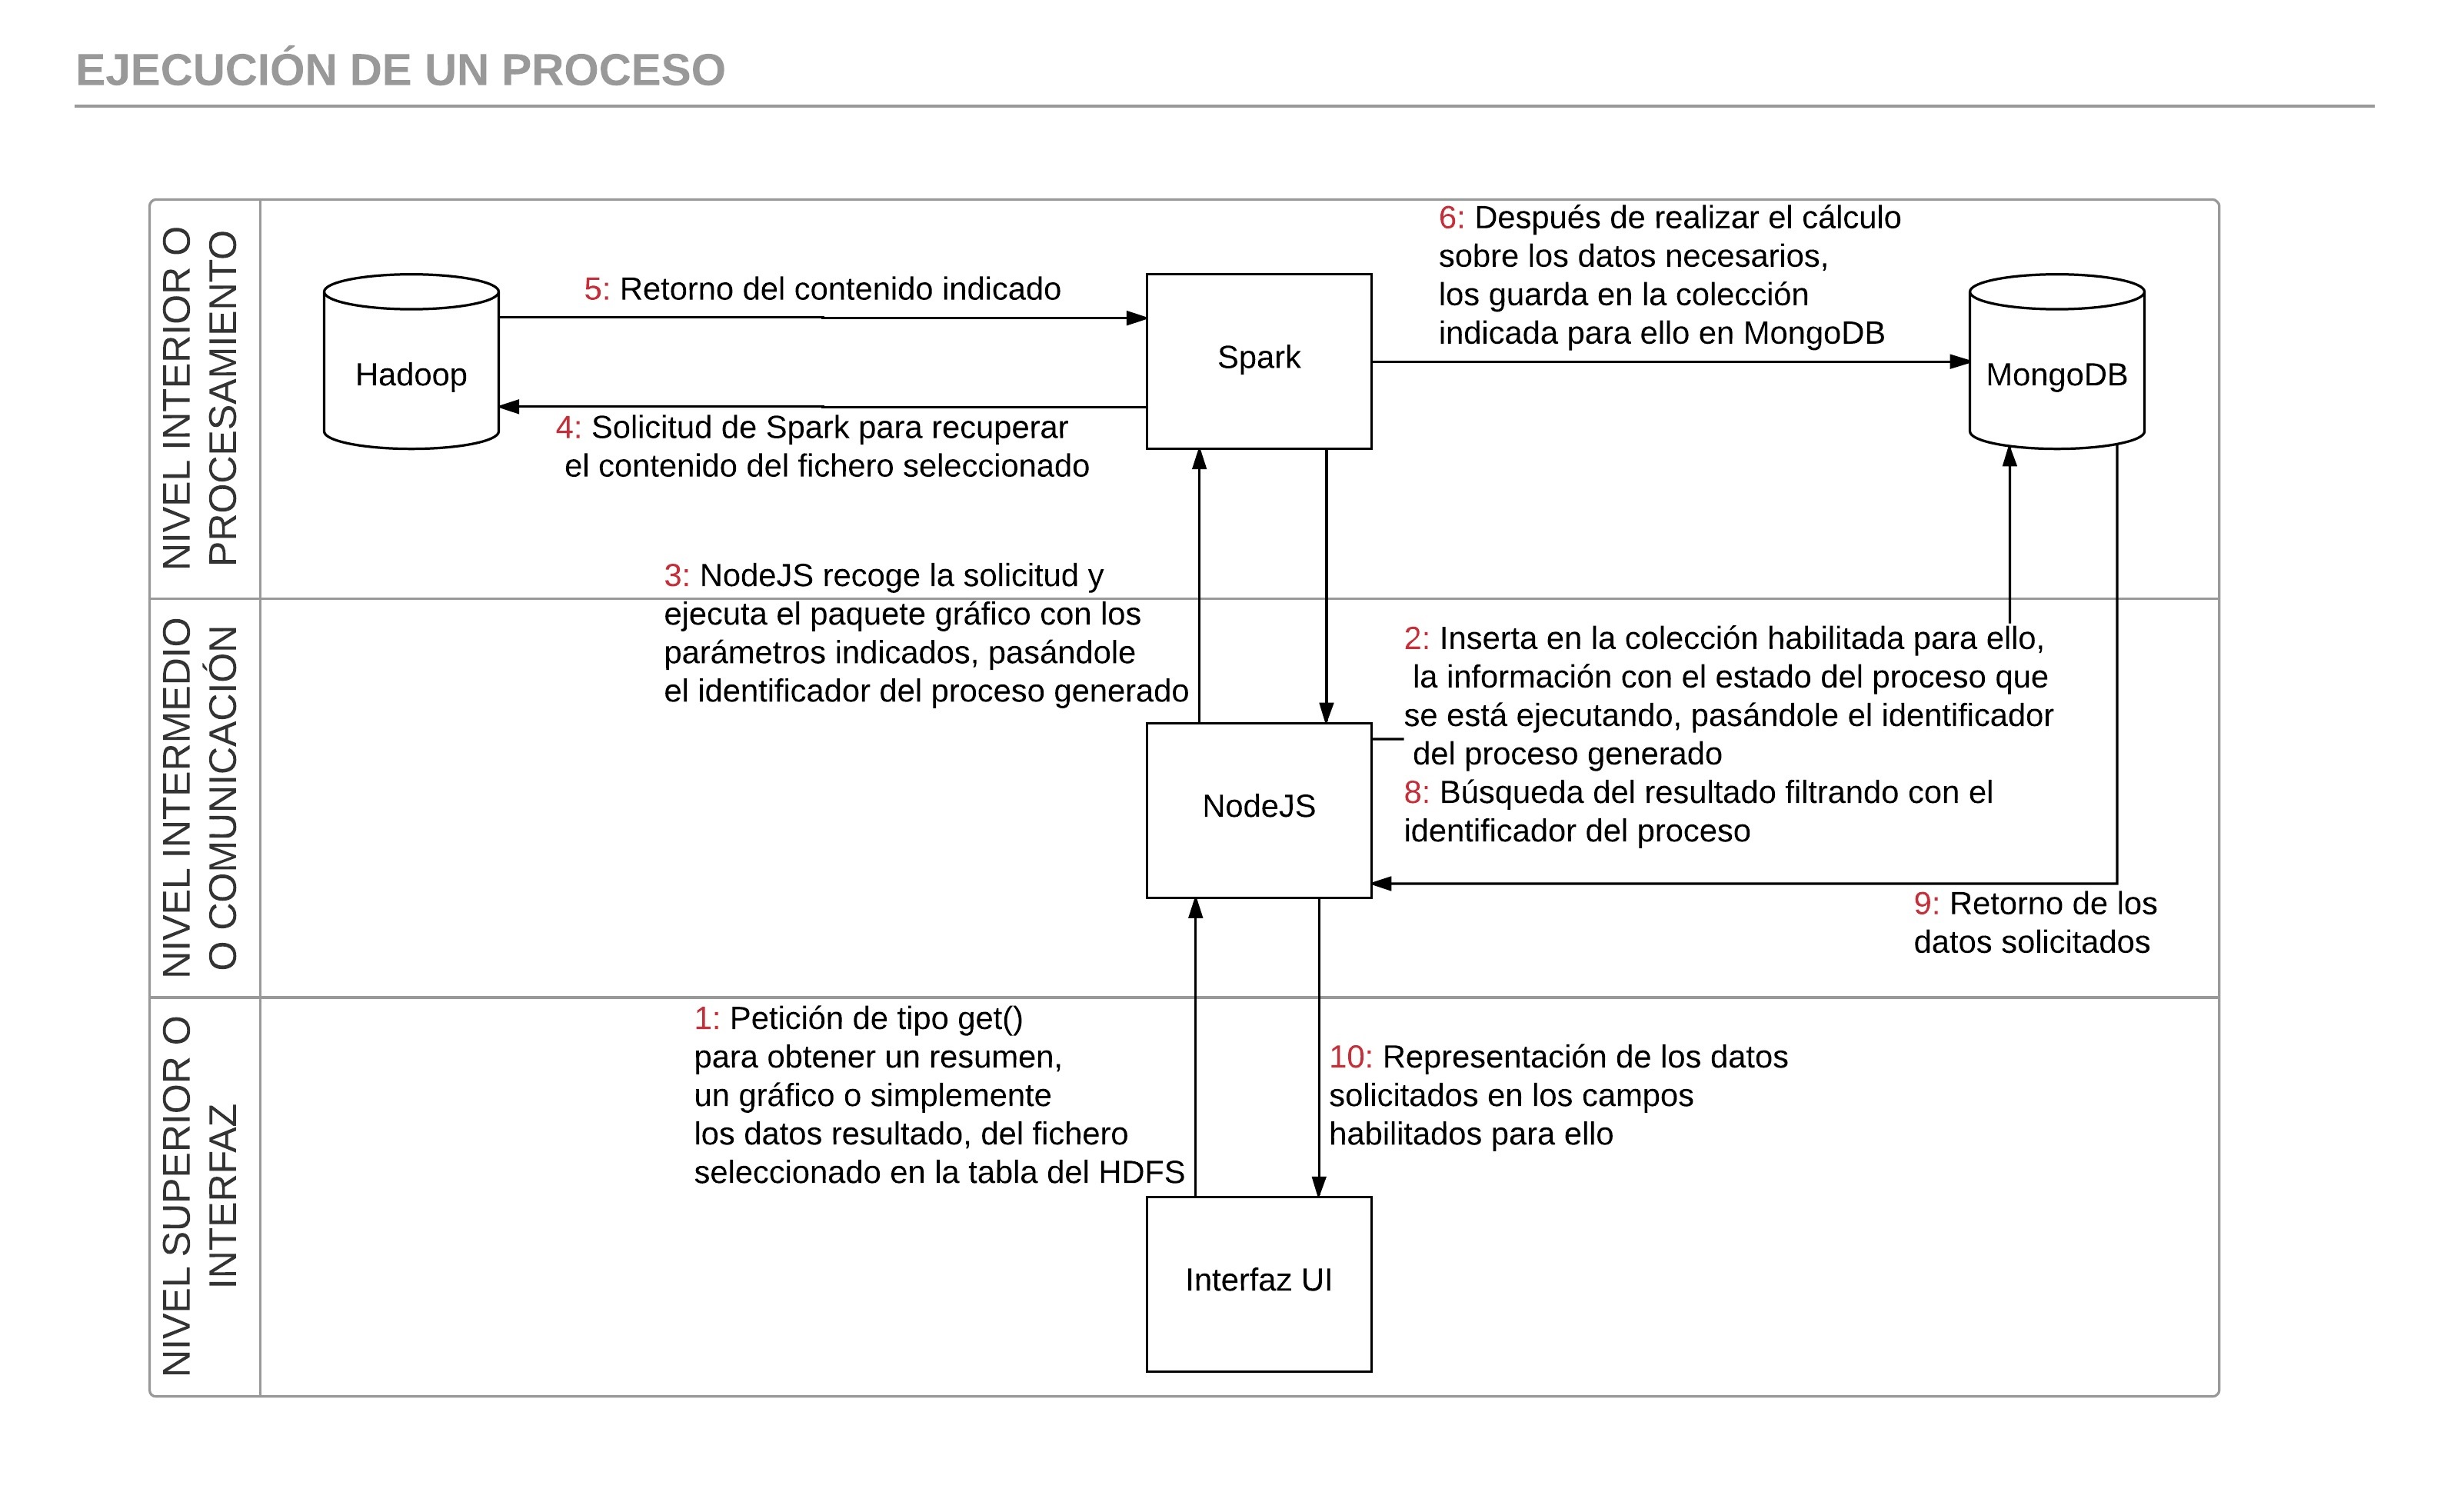
\includegraphics[width=1\linewidth]{imagenes/Ejecucion_de_un_proceso}
	\caption{Ejecución de un proceso solicitado}
	\label{fig:ejecuciondeunproceso}
\end{figure}

Ejecutar el paquete gráfico es el siguiente paso, enviándole la información de los parámetros indicada anteriormente, junto con el identificador. 

Dentro del paquete en Spark, como ya se explicó, primero se recupera el archivo del HDFS. En el caso del paquete ‘summary’, basta con obtener algunos metadatos del fichero, como la cantidad de columnas que contiene, los nombres de las mismas o el número de registros, entre otros. Si se está ejecutando un proceso gráfico, entonces el propio paquete contendrá el esquema de agrupación y las técnicas de reducción de datos que debe ejecutar para obtener el resultado correcto. Finalizado este cálculo, Spark guarda en la colección de MongoDB, el resultado junto al identificador del proceso. 

Cuanto termina de ejecutarse la librería, NodeJS busca el resultado en MongoDB, utilizando como filtro el identificador. Por último, regresará la información a la interfaz para visualizarla en los campos indicados para ello.

\section{Instalación del sistema de visualización y BigData}

Como ya se han explicado con anterioridad, los componentes necesarios para la utilización de la API son:
\begin{itemize}
	\item Spark (2.0)
	\item Hadoop (2.6)
	\item Scala (2.11)
	\item Java JDK (1.7 o superior)
	\item MongoDB (3.2)
	\item NodeJS (6.9)
	\item Sbt (0.13)
\end{itemize}

Cabe destacar que es posible que se pueda instalar la API con otras versiones de alguna de las herramientas listadas anteriormente, pero no se garantiza la correcta funcionalidad de la misma.

Es posible una instalación básica del sistema de todos estos componentes de manera automática, excepto de Hadoop, mediante el fichero installAll.sh, proporcionado dentro del directorio del proyecto en GitHub, para sistemas CentOS, Fedora, RedHat, etc. Esta instalación está basada en los requisitos mínimos para que el sistema funcione, en un solo nodo para Hadoop y Spark. La instalación de Hadoop es más complicada y por ello se debe realizar manualmente. En sistemas Debian, la instalación debe ser manual. La única diferencia es el cambio en los nombres de algunos de los comando utilizados en sistemas Debian. La instalación básica requiere de al menos 8 GB de RAM y al menos ocupa 4GB de espacio en disco.

\underline{Importante}: Para que el sistema funcione con el firewall activado, es necesario tener abiertos los puertos que solicita cada una de las herramientas como Hadoop, Spark, etc. En caso contrario, se deshabilitara el firewall para poder ejecutar la API sin ese problema. Los siguientes comando lo deshabilitan para Centos 7. (Estos comandos ya están añadidos en el fichero installAll.sh)

\begin{verbatim}
	systemctl disable firewalld
	
	systemctl stop firewalld
\end{verbatim}

También es importante abrir el puerto del ordenador o cluster que se le indique en la configuración de la API.

Para la instalación de Hadoop y Spark sobre un cluster de varios nodos, se ha seguido el siguiente tutorial \cite{InstalacionHadoopSparkNodos} proporcionado por el tutor del proyecto. La instalación de NodeJS y el resto de componentes se realiza de la misma forma que en la versión básica explicada anteriormente. 

\section{Compilación de los paquetes gráficos}

Para que el sistema pueda ejecutar cada uno de los paquetes que calculan los datos resultados necesarios para los gráficos, es necesario tener instaladas las siguientes herramientas como mínimo:
\begin{itemize}
	\item Spark
	\item MongoDB
	\item Hadoop
	\item Scala
\end{itemize}

Lo primero es compilar el paquete. Dentro del proyecto ya vienen compiladas las funciones de cada uno de los gráficos, pero si se realizan cambios sobre el código de alguno de ellos, es necesario volver a compilar. 

Para ello, es necesario situarse dentro del directorio del gráfico (histogram, boxplot, ...) y utilizar el comando "sbt assembly". A continuación, se generará un paquete .jar en ./target/scala-2.11/X-assembly-1.0.jar, donde X será el nombre del gráfico a compilar y dependiendo de la versión de Scala que esté instalada. Este paquete contendrá todas las librerías privativas necesarias para su correcto funcionamiento, indicadas dentro del fichero ‘build.sbt’, en el directorio de cada uno de los gráficos.

Dentro de estos directorios, existe un ejecutable 'launch.sh', donde se puede probar la funcionalidad del mismo paquete, con algunos datos de prueba. En la sección número 6 de este documento, se especifica que parámetros se deben introducir en cada uno de los gráficos. Tener en cuenta que se necesitan datos dentro del HDFS y que el resultado de la ejecución, se guardará en MongoDB, además de ajustar los parámetros de conexión a las condiciones de cada servidor y de cada ejecución.

\section{Uso de la biblioteca}

Durante el desarrollo del sistema, se ha utilizado una herramienta de documentación y testeo sobre NodeJS llamada \textbf{Swagger} \cite{SwaggerInicial}. Este programa permite crear documentación online de cada una de la funcionalidad implementada, y comprobar si se obtienen los resultados correctamente de una manera muy interactiva.

Para ver la documentación que ofrece Swagger, previamente diseñada por el programador dentro de NodeJS, es necesario ejecutar en un terminal Linux dentro del sistema y dentro también del directorio donde se encuentre el proyecto, el siguiente comando:

\begin{verbatim}
	swagger project edit
\end{verbatim}

Se abrirá una nueva ventana en el navegador donde se podrá ver la información sobre cada una de las funcionalidades de la API. Ahora, para poder lanzar la API desde un terminal Linux, es necesario ejecutar el siguiente comando dentro del directorio donde se encuentre.

\begin{verbatim}
	swagger project start
\end{verbatim}

Si no se desea instalar Swagger, ya que es opcional, simplemente se puede lanzar el siguiente comando para ejecutar la API 

\begin{verbatim}
	node app.js
\end{verbatim}

El problema de ejecutar este comando es que al terminar la sesión en el terminal donde se ejecutó, se cancela la ejecución del sistema. Por eso es necesario utilizar algún otro comando o programa que permita dejar funcionando el sistema aunque se termine la sesión. Para lograr este objetivo se puede utilizar el comando ‘nohup’ de la siguiente forma.

\begin{verbatim}
	nohup node app.js &
\end{verbatim}

Así permanecerá el sistema iniciado hasta que el administrador del equipo decida terminar con el proceso. Este comando tiene un pequeño inconveniente y es que no es capaz de recuperarse ante un error de la aplicación y volver a ejecutarlo. Por eso se recomienda instalar la librería \textbf{Forever} \cite{ForeverInicial}, a través del gestor de paquetes NPM. Forever tiene la capacidad de reiniciar el sistema si se produjera un error en algún momento. Se puede lanzar con el siguiente comando:

\begin{verbatim}
	forever node app.js
\end{verbatim}

También se puede combinar el comando para lanzar Swagger con Forever.
Aparte de la ejecución, instalando el monitor \textbf{Forever-Monitor} \cite{ForeverMonitor} se puede programar la ejecución para que responda a los parámetros indicados. Esto es opcional por parte del administrador del sistema.

Finalmente, hay una instalación del sistema totalmente funcionando en la siguiente dirección, para que pueda ser probada toda la funcionalidad implementada con unos datos de prueba:

\begin{verbatim}
	http://docker.ugr.es:30183/
\end{verbatim}

\subsection{API RESTful y documentación con Swagger}

Gracias a la librería Swagger \cite{SwaggerInicial}, se ha podido generar una API RESTful donde se puede comprobar el funcionamiento de cada una de los métodos implementados en el sistema, como se puede apreciar en la figura \ref{fig:swaggerfunciones} del capítulo anterior. Además, cada uno de estos métodos como sus parámetros están correctamente documentado, lo que permite entenderlos de manera más clara. Un ejemplo es la función que calcula el resultado para el histograma (ver figura \ref{fig:swaggerhistograma} del capítulo anterior). Al ser una API RESTful, se puede probar el funcionamiento de cada uno y como resultado, obtener los datos calculados en vez de visualizarlos en un gráfico.

En el siguiente capítulo se explica en detalle cada una de las funciones gráficas del sistema y para que sirven cada uno de sus parámetros.






\chapter{Métodos de Visualización Empleados}

En esta sección se discutirán los distintos métodos empleados, sobre cada uno de los gráficos, para analizar los datos seleccionados y elegir una técnica de reducción óptima para cada uno de los gráficos. Cada infograma es distinto al anterior, ya que representa información distinta y la estructura de diferente manera. Por eso no es posible aplicar las mismas técnicas sobre todos. Cada uno debe ser analizado específicamente para conocer cuáles son sus límites a la hora de dibujarlo, los tipos de datos que es capaz de representar y, que operaciones sobre los datos representan fielmente lo que quieren contar.

Los siguientes apartados se centrarán en explicar cómo funcionan cada uno de los gráficos disponibles en la API, que técnicas se han utilizado para reducir la cantidad de datos y resumirlos de forma que sean lo más representativos y, qué parámetros son necesarios indicarles para ejecutarlos. Todas las funciones se realizan mediante peticiones de tipo \textit{get}. Cabe destacar que cada uno de los gráficos que se generan son adaptativos a la resolución del dispositivo en el que se esté usando la API.

A continuación, se puede apreciar un listado con todos los gráficos disponibles en la API y que se explican en detalle posteriormente:
\begin{itemize}
	\item Histograma
	\item Boxplot
	\item Scatterplot
	\item Heatmap
	\item Bubble Chart
	\item Scatterplot Matrix
	\item Pie Chart
	\item Line Chart
	\item Stacked Area Chart
	\item Bar Chart
\end{itemize}

\section{Cuestiones generales sobre la visualización}
Como ya se ha explicado anteriormente, todo el sistema está desarrollado para funcionar sobre conjuntos de datos 'Big Data'. Esto conlleva que los cálculos sobre esos conjuntos de datos sea realmente la dificultad que tiene este proyecto. Para obtener una representación gráfica, por ejemplo un histograma o un boxplot, es necesario obtener unos valores calculados como máximo, mínimo, cuartiles, agrupaciones, conteo de datos, etc. Aquí es donde realmente está la complejidad de representar un histograma en comparación con otras herramientas clásicas, sobre conjuntos de datos de menor tamaño. 

Spark provee funcionalidad que permite calcular estas operaciones o parte de ellas de manera rápida y eficaz, pero lo interesante de este proyecto es la utilización de estas herramientas, para obtener los valores y a continuación, crear un gráfico representativo de lo que ocurre con el conjunto 'Big Data'.

En las siguientes secciones, se van a exponer cada uno de los gráficos implementados, explicando los pasos seguidos y los cálculos necesarios para dibujarlos.

\section{Histograma}
La idea del histograma es la de contabilizar los valores de una o varias columnas de un grupo de datos. Se pueden elegir la cantidad de agrupaciones o segmentos basados de los registros de los datos. Esta será la cantidad de columnas que tendrá el histograma. 

Una vez elegidos cuantos segmentos se necesitan, se calculan los limites de cada uno de ellos. Para ello, es necesario obtener el máximo y mínimo valor de todos los registros de los datos en la columna seleccionada, y aplicar la siguiente operación:

\begin{verbatim}
	(Máximo – Mínimo) / Número de segmentos = Amplitud de cada segmento
\end{verbatim}

Con la amplitud de cada uno de los segmentos, se obtienen los límites de cada uno, es decir, el máximo y mínimo valor de cada uno donde deben estar agrupados los valores. A continuación, se filtran los valores de las columnas seleccionadas y se contabilizan. Sólo queda guardar los resultados en JSON para su posterior representación gráfica.

Hay que tener en cuenta que el límite para elegir el número de segmentos son la cantidad de píxeles del gráfico en la pantalla, por esa razón se agrupan los valores a representar. Se puede ver un ejemplo en la figura \ref{fig:ejemplohistograma}
\begin{figure}
	\centering
	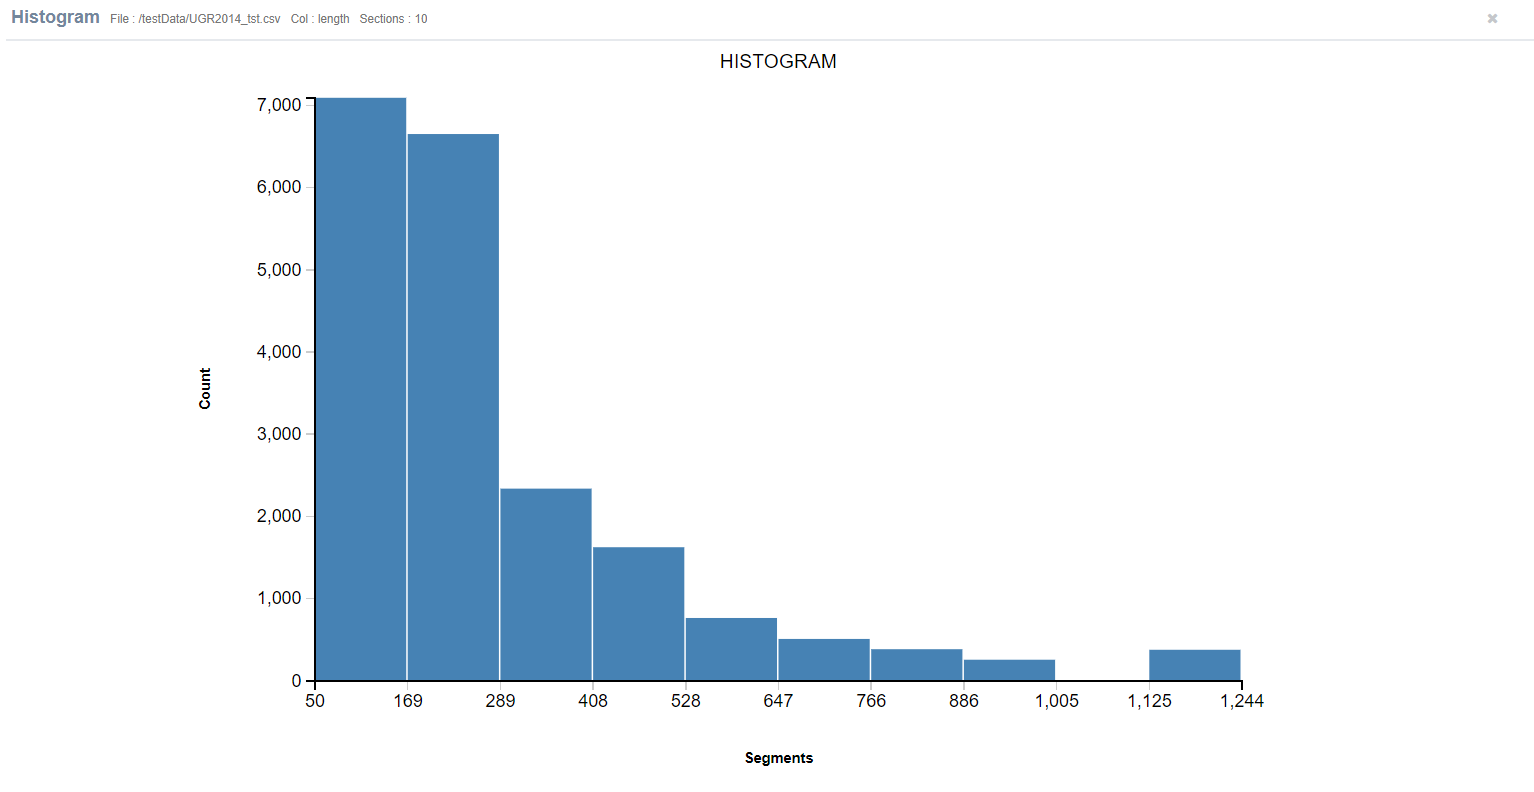
\includegraphics[width=1\linewidth]{imagenes/ejemplo_histograma}
	\caption{Ejemplo de un histograma}
	\label{fig:ejemplohistograma}
\end{figure}

Para la ejecución del histograma (ejemplo de URL\footnotemark), los parámetros por orden de inserción son:

\begin{tabular}{|l|l|p{7cm}|}
	\hline 
	\textbf{Campo} & \textbf{Tipo} & \textbf{Descripción} \\ 
	\hline \hline
	\multicolumn{3}{|c|}{\textit{Datos que proporciona la API}} \\
	\hline 
	MongoURL & String & URL del servidor MongoDB activo \\ 
	\hline 
	MongoDB & String & Base de datos dentro de MongoDB \\ 
	\hline 
	MongoCollect& String & Colección dentro de la base de datos en MongoDB \\ 
	\hline \hline
	\multicolumn{3}{|c|}{\textit{Datos que proporciona el usuario}} \\
	\hline 
	File & String & Fichero de entrada de datos, con formato CSV, situado en el HDFS (Hadoop) \\ 
	\hline 
	Col & String & Nombre de la columna del fichero de datos que se quiere analizar \\ 
	\hline 
	Sec & Number & Número de segmentos o intervalos en los que dividir los datos \\ 
	\hline 
\end{tabular} 

\footnotetext{/histogram?file=\%2FtestData\%2F1000\_ECBDL14\_10tst.csv\&col=f3\&sections=5}

\section{Boxplot}
El infograma boxplot se utiliza para representar las características principales de una distribución de valores. Estas características dan información acerca del comportamiento de los datos, en su conjunto, para una columna concreta del fichero. De cada uno de esas distribuciones o columnas de registros, lo primero es ordenar los datos de manera ascendente, para después calcular los siguientes valores:
\begin{itemize}
	\item Valor mínimo
	\item Primer cuartil
	\item Mediana
	\item Tercer cuartil
	\item Valor máximo
	\item IQR
\end{itemize}

Estas características son las que mejor representan el comportamiento de un conjunto de datos. El primer cuartil es el valor que para los que el 25\% de los valores ordenados son más pequeños que él. De manera opuesta, el tercer cuartil es el valor que representa que el 75\% de los valores son más pequeños. Después, la mediana representa el valor intermedio del conjunto de datos, lo que indica que el 50\% tienen valores más pequeños y el otro 50\% contiene registros mayores. El rango intercuartílico, o IQR, es la diferencia entre el tercer y primer cuartil del conjunto de datos. Sirve para eliminar algunos valores del conjunto que están extremadamente alejados y dispersos.

Spark implementa funciones específicas para calcular cada uno de estos valores sobre un Dataframe. Así, solo basta con utilizarlas para obtener los valores. Se puede ver un ejemplo en la figura \ref{fig:ejemploboxplot}
\begin{figure}
	\centering
	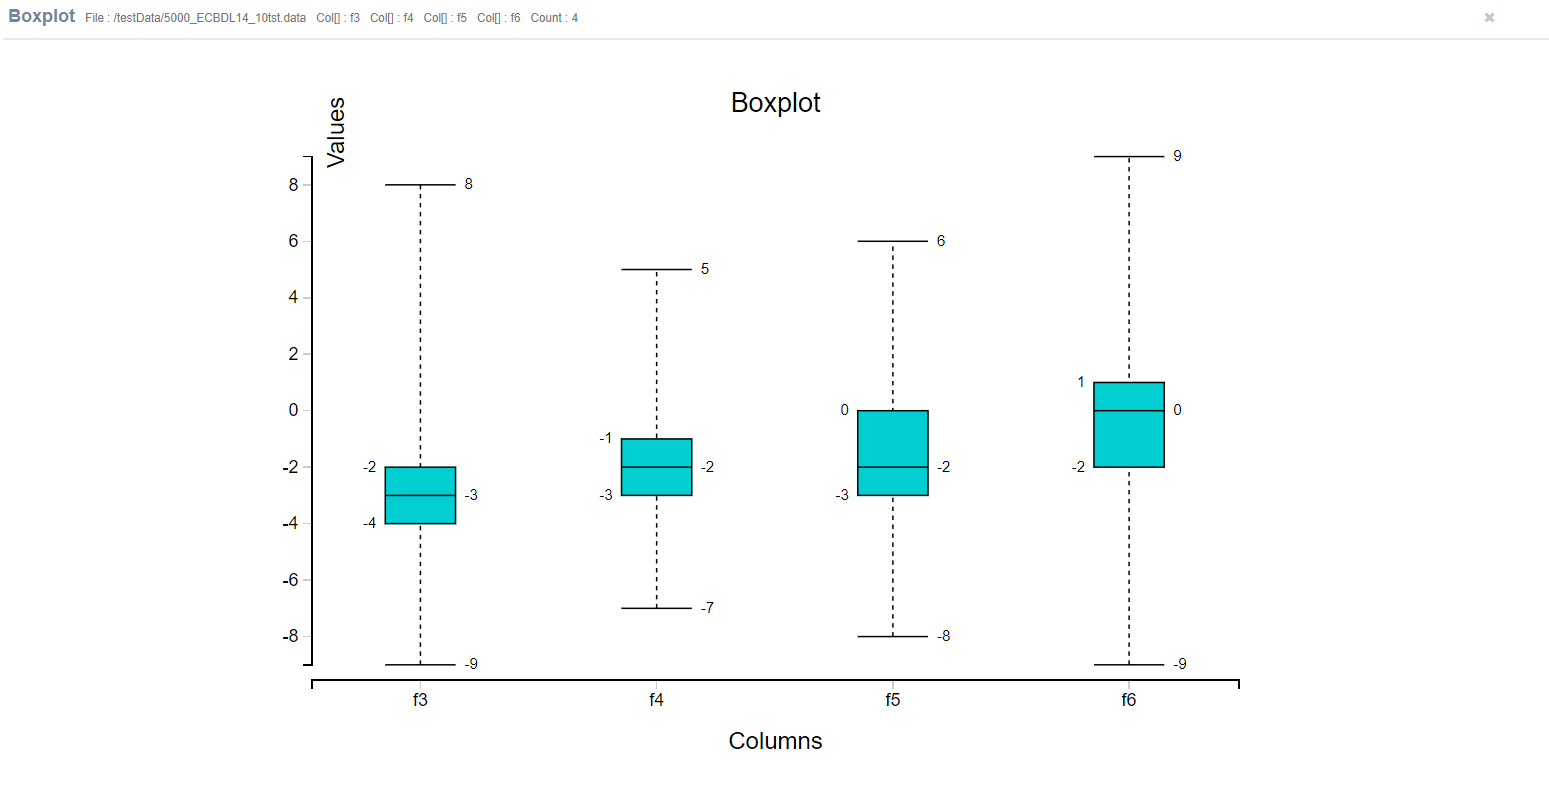
\includegraphics[width=1\linewidth]{imagenes/ejemplo_boxplot}
	\caption{Ejemplo del gráfico boxplot}
	\label{fig:ejemploboxplot}
\end{figure}

Para la ejecución del boxplot (ejemplo de URL\footnotemark), los parámetros por orden de inserción son:

\begin{tabular}{|l|l|p{7cm}|}
	\hline 
	\textbf{Campo} & \textbf{Tipo} & \textbf{Descripción} \\ 
	\hline \hline
	\multicolumn{3}{|c|}{\textit{Datos que proporciona la API}} \\
	\hline 
	MongoURL & String & URL del servidor MongoDB activo \\ 
	\hline 
	MongoDB & String & Base de datos dentro de MongoDB \\ 
	\hline 
	MongoCollect& String & Colección dentro de la base de datos en MongoDB \\ 
	\hline \hline
	\multicolumn{3}{|c|}{\textit{Datos que proporciona el usuario}} \\
	\hline 
	File & String & Fichero de entrada de datos, con formato CSV, situado en el HDFS (Hadoop) \\ 
	\hline 
	Count & Number & Numero de columnas del fichero a representar \\ 
	\hline 
	Col & Array[String] & Array con el nombre de las columnas del fichero seleccionadas \\ 
	\hline 
\end{tabular} 

\footnotetext{/boxplot?file=\%2FtestData\%2F1000\_ECBDL14\_10tst.csv\&count=3\&col=f3,f4,f5}

\section{Scatterplot}
El gráfico scatterplot está diseñado para representar pares de datos mediante puntos sobre un eje de coordenadas. Cada uno de los datos representa una posición sobre el eje correspondiente. Es una representación gráfica muy útil para averiguar si los datos siguen un determinado patrón, o por el contrario, simplemente no constata ningún comportamiento específico.

Aplicado al Big Data, reducir el número de datos a representar es fundamental, ya que dibujar todos y cada uno de los datos puede llegar a ser costoso y difícil de analizar su comportamiento. Dicho esto, es necesario buscar una solución de agrupación de los datos, sin perder información.

La técnica que se ha aplicado en este caso es dividir los ejes en secciones, de un tamaño variable, para que los datos estuvieran sobre una matriz. El siguiente paso ha sido averiguar en qué sección cae cada uno de los datos. Para hace esto de manera eficiente, se ha aplicado el siguiente algoritmo:
\begin{itemize}
	\item Se calcula el máximo y mínimo de cada uno de los ejes (grupo de datos)
	\item Obtenemos el tamaño de cada sección de la matriz por eje:
	\begin{verbatim}
		Tamaño de la sección = (Máximo – Mínimo) / Número de secciones
	\end{verbatim}
	\item Calculamos a que sección pertenece cada punto por eje:
	\begin{verbatim}
		Valor absoluto ((valor X - Mínimo) / Tamaño de la sección)
	\end{verbatim}
\end{itemize}

De esta manera, es posible saber en qué sección de la matriz cae cada uno de los puntos. Por último, contar cuantos puntos pertenecen a cada uno de las secciones de la matriz y calcular el centroide. Así, es posible reducir el número de datos a representar sin perder demasiada información de los mismos.

Como añadido, se ha insertado una gama de colores en la representación gráfica según la cantidad de puntos agrupados por secciones, para así facilitar la densidad de registros en ciertas zonas del gráfico.  Se puede ver un ejemplo en la figura \ref{fig:ejemploscatterplot}
\begin{figure}
	\centering
	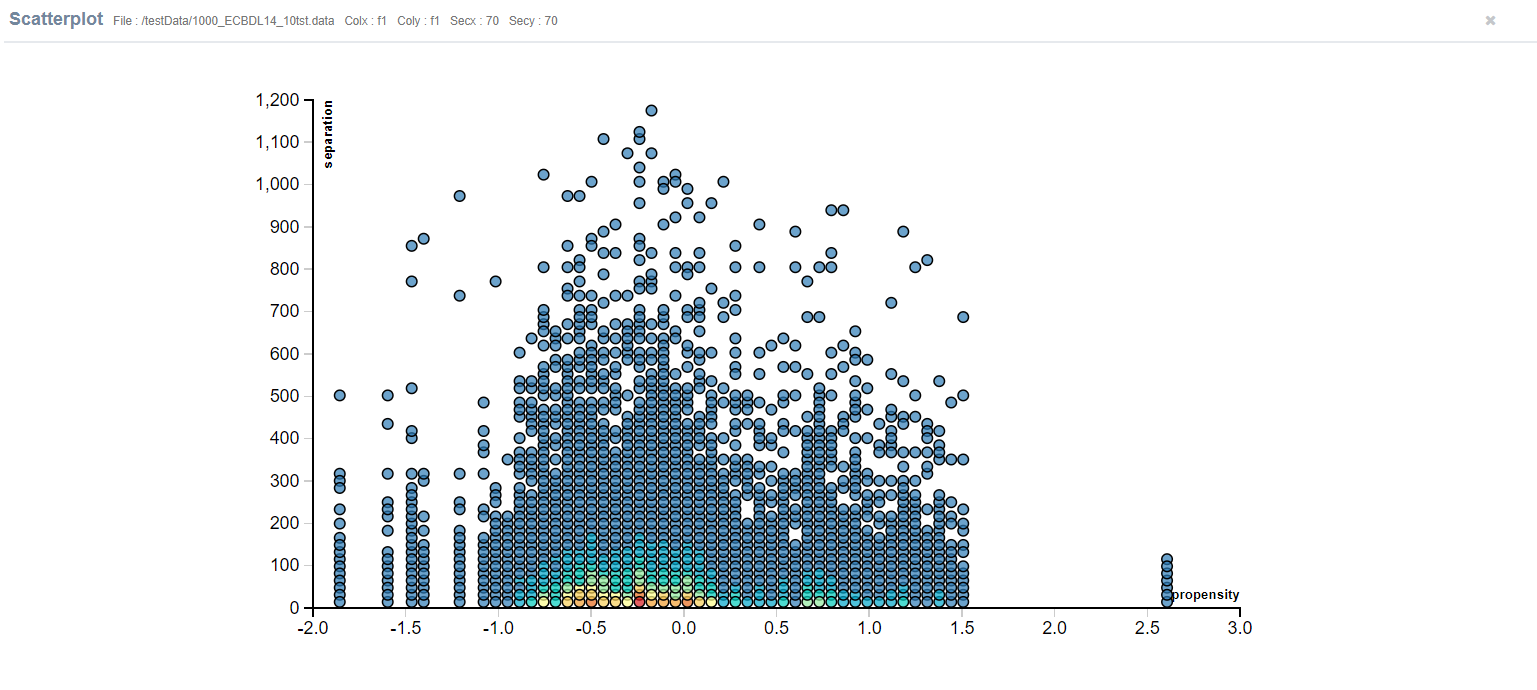
\includegraphics[width=1\linewidth]{imagenes/ejemplo_scatterplot}
	\caption{Ejemplo de scatterplot}
	\label{fig:ejemploscatterplot}
\end{figure}

Para la ejecución del scatterplot (ejemplo de URL\footnotemark), los parámetros por orden de inserción son:

\begin{tabular}{|l|l|p{7cm}|}
	\hline 
	\textbf{Campo} & \textbf{Tipo} & \textbf{Descripción} \\ 
	\hline \hline
	\multicolumn{3}{|c|}{\textit{Datos que proporciona la API}} \\
	\hline 
	MongoURL & String & URL del servidor MongoDB activo \\ 
	\hline 
	MongoDB & String & Base de datos dentro de MongoDB \\ 
	\hline 
	MongoCollect& String & Colección dentro de la base de datos en MongoDB \\ 
	\hline \hline
	\multicolumn{3}{|c|}{\textit{Datos que proporciona el usuario}} \\
	\hline 
	File & String & Fichero de entrada de datos, con formato CSV, situado en el HDFS (Hadoop) \\ 
	\hline 
	Colx & String & Columna de datos a representar como eje X \\ 
	\hline 
	Coly & String & Columna de datos a representar como eje Y \\ 
	\hline 
	Secx & Number & Número de secciones en el eje X para la matriz \\ 
	\hline 
	Secy & Number & Número de secciones en el eje Y para la matriz \\ 
	\hline 
\end{tabular} 

\footnotetext{/scatterplot?file=\%2FtestData\%2F1000\_ECBDL14\_10tst.csv\&colx=f3\&coly=f4\&secx=10\&secy=10}

\section{Heatmap}
El infograma Heatmap representa los datos en un formato de tabla con una gama de colores definida en base a una frecuencia u operación, desde colores que representan valores bajos hasta altos. Esta representación basada en colores hace que el gráfico sea mucho más fácil de entender y, por tanto, comprender mejor lo que indican los datos.

En la API, se seleccionan las columnas que van a representar los ejes X e Y, la columna de datos numéricos que calcular y el tipo de operación sobre dicha columna. Lo primero es agrupar los valores de las columnas seleccionados en variables de tipo ‘key-value’, tal que la clave esté formada por los valores de las columnas de los ejes, sin repeticiones, y el valor sea la columna elegida a representar, con la operación seleccionada aplicada, ya sea sumar, encontrar el valor máximo o encontrar el valor mínimo. Estas operaciones vienen implementadas por defecto en Spark para poder calcular estos valores. La dificultad del Big Data en este caso es que puede llegar a agruparse un número muy grande de registros, pero para ello también hay funciones de Spark que realizan estas agrupaciones, paralelizando el proceso, obteniendo más velocidad de cómputo.

Para los colores se ha aplicado la misma técnica que se utiliza en el gráfico Scatterplot.  Se puede ver un ejemplo en la figura \ref{fig:ejemploheatmap}
\begin{figure}
	\centering
	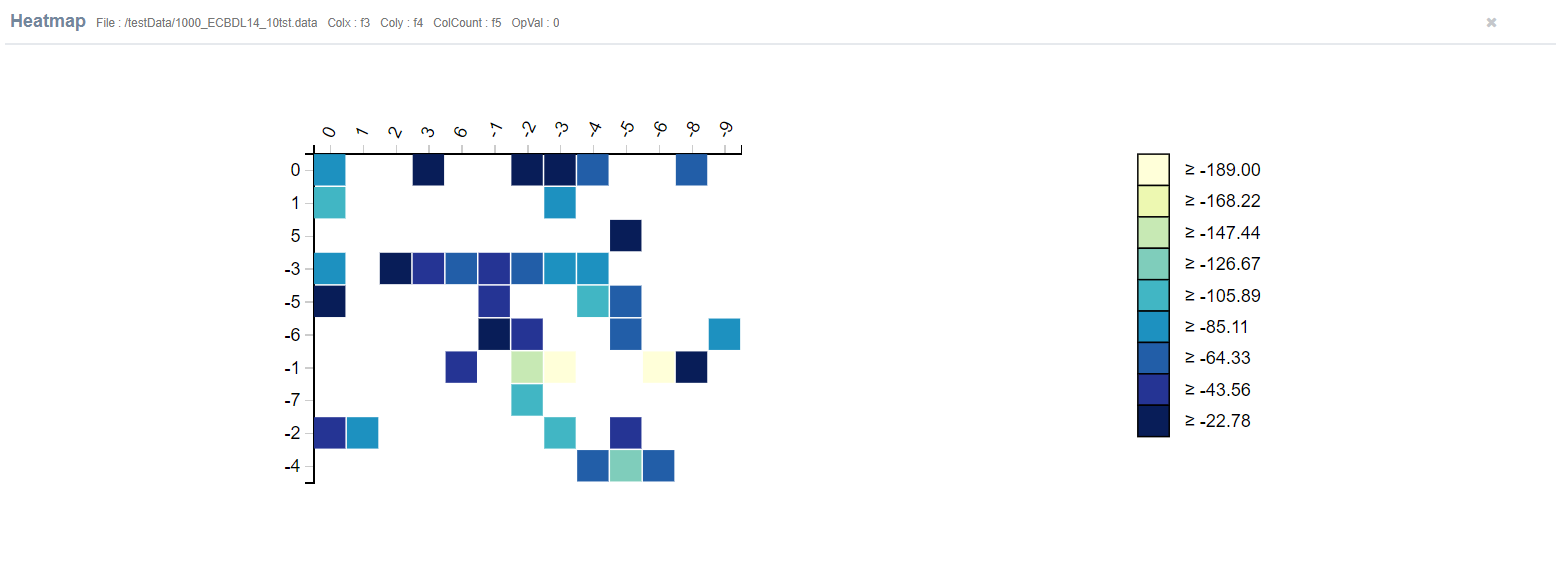
\includegraphics[width=1\linewidth]{imagenes/ejemplo_heatmap}
	\caption{Ejemplo de heatmap}
	\label{fig:ejemploheatmap}
\end{figure}

Para la ejecución del heatmap (ejemplo de URL\footnotemark), los parámetros por orden de inserción son:

\begin{tabular}{|l|l|p{7cm}|}
	\hline 
	\textbf{Campo} & \textbf{Tipo} & \textbf{Descripción} \\ 
	\hline \hline
	\multicolumn{3}{|c|}{\textit{Datos que proporciona la API}} \\
	\hline 
	MongoURL & String & URL del servidor MongoDB activo \\ 
	\hline 
	MongoDB & String & Base de datos dentro de MongoDB \\ 
	\hline 
	MongoCollect& String & Colección dentro de la base de datos en MongoDB \\ 
	\hline \hline
	\multicolumn{3}{|c|}{\textit{Datos que proporciona el usuario}} \\
	\hline 
	File & String & Fichero de entrada de datos, con formato CSV, situado en el HDFS (Hadoop) \\ 
	\hline 
	Colx & String & Columna de datos a representar como eje X \\ 
	\hline 
	Coly & String & Columna de datos a representar como eje Y \\ 
	\hline 
	Colcount & String & Columna de datos para representar el valor \\ 
	\hline 
	Opval & Number & Código de la operación para ser aplicada  [0-Sum, 1-Max, 2-Min] \\ 
	\hline 
\end{tabular} 

\footnotetext{/heatmap?file=\%2FtestData\%2F1000\_ECBDL14\_10tst.csv\&colx=f3\&coly=f4\&colCount=f5\&opVal=0}

\section{Bubble Chart}
El gráfico Bubble Chart está basado en el mismo algoritmo que el gráfico Scatterplot. Los datos se ejecutan de la misma forma que al aplicar el Scatterplot, cambiando únicamente la representación gráfica.

La diferencia principal del Bubble Chart es al representar los puntos del gráfico con tamaños diferentes, e incluso con colores diferentes, para enfatizar más la densidad de datos que se localizan en una zona concreta. Si hay muchos datos en una zona, aumenta el interés en esa zona y, por tanto, se representa con un círculo de mayor tamaño en comparación con otras zonas en las que existen menos puntos de datos.

Para calcular el tamaño de los círculos, se ha aplicado el mismo algoritmo que se utiliza para los colores en el gráfico Scatterplot, cambiando la densidad de puntos que se representa por un color, por un aumento en el radio del círculo.  Se puede ver un ejemplo en la figura \ref{fig:ejemplobubblechart}
\begin{figure}
	\centering
	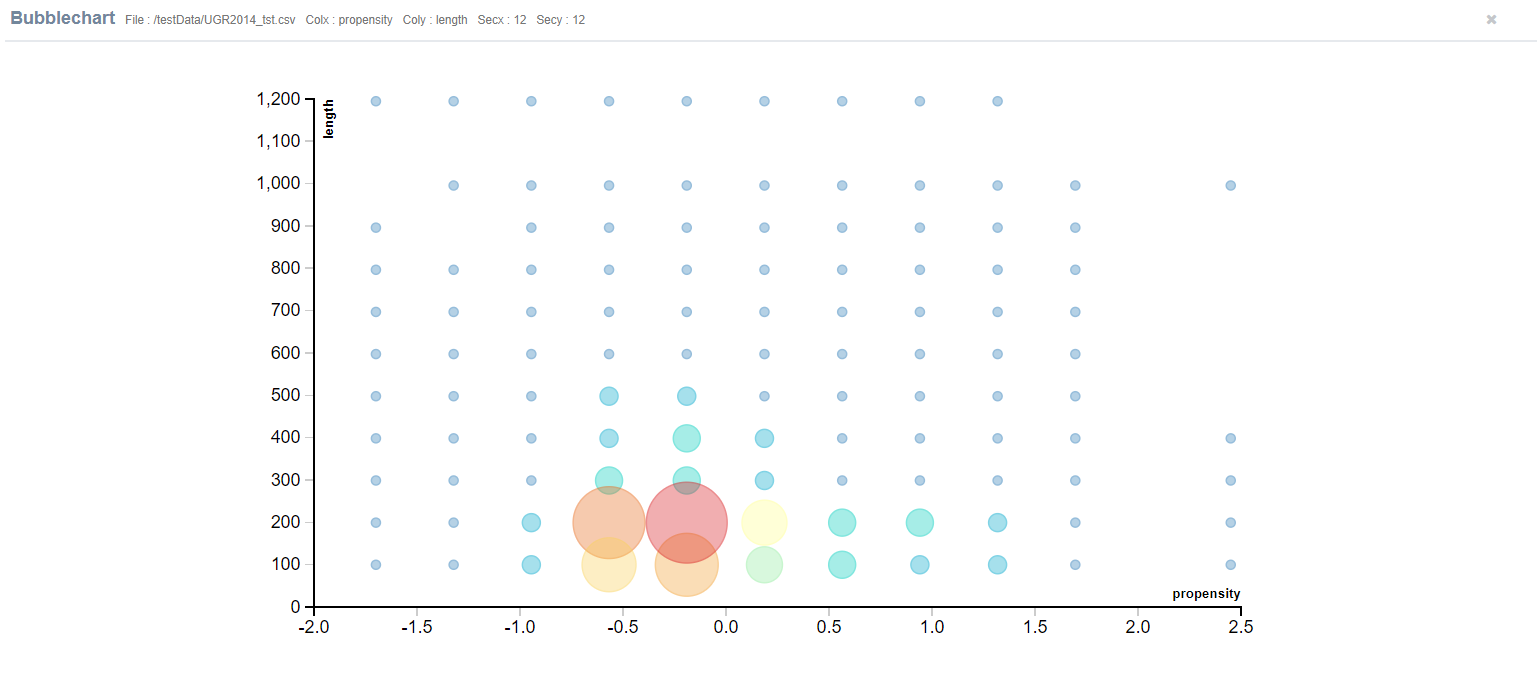
\includegraphics[width=1\linewidth]{imagenes/ejemplo_bubblechart}
	\caption{Ejemplo de un bubble chart}
	\label{fig:ejemplobubblechart}
\end{figure}

Para la ejecución del bubble chart (ejemplo de URL\footnotemark), los parámetros por orden de inserción son:

\begin{tabular}{|l|l|p{7cm}|}
	\hline 
	\textbf{Campo} & \textbf{Tipo} & \textbf{Descripción} \\ 
	\hline \hline
	\multicolumn{3}{|c|}{\textit{Datos que proporciona la API}} \\
	\hline 
	MongoURL & String & URL del servidor MongoDB activo \\ 
	\hline 
	MongoDB & String & Base de datos dentro de MongoDB \\ 
	\hline 
	MongoCollect& String & Colección dentro de la base de datos en MongoDB \\ 
	\hline \hline
	\multicolumn{3}{|c|}{\textit{Datos que proporciona el usuario}} \\
	\hline 
	File & String & Fichero de entrada de datos, con formato CSV, situado en el HDFS (Hadoop) \\ 
	\hline 
	Colx & String & Columna de datos a representar como eje X \\ 
	\hline 
	Coly & String & Columna de datos a representar como eje Y \\ 
	\hline 
	Secx & Number & Número de secciones en el eje X para la matriz \\ 
	\hline 
	Secy & Number & Número de secciones en el eje Y para la matriz \\ 
	\hline 
\end{tabular} 

\footnotetext{/bubblechart?file=\%2FtestData\%2F1000\_ECBDL14\_10tst.csv\&colx=f3\&coly=f4\&secx=10\&secy=10}

\section{Scatterplot Matrix}
El infograma Scatterplot Matrix es muy útil para determinar si existe algún tipo de correlación lineal entre un número determinado de variables. Saber que variables pueden contener alguna relación entre sí, o simplemente conocer que no aportan ningún tipo de información de valor, es de gran ayuda al analizar grandes cantidades de datos. El gráfico Scatterplot Matrix permite, de un solo vistazo, conocer esta información, para a continuación, entrar más en detalle con un Scatterplot sobre esas variables de interés.

Como ocurre con el gráfico Bubble Chart, el algoritmo para calcular cada uno de los cruces entre variables en el Scatterplot Matrix, es el mismo que el de Scatterplot. En esta ocasión, en vez de elegir dos columnas de los datos que representen cada uno de los ejes, se escogen un rango de variables que el usuario pueda conocer que sean de interés, y el algoritmo calculará cada uno de los cruces entre los mismos, con el fin de conocer si existe una correlación lineal entre varias. Se puede ver un ejemplo en la figura \ref{fig:ejemploscatterplotmatrix}
\begin{figure}
	\centering
	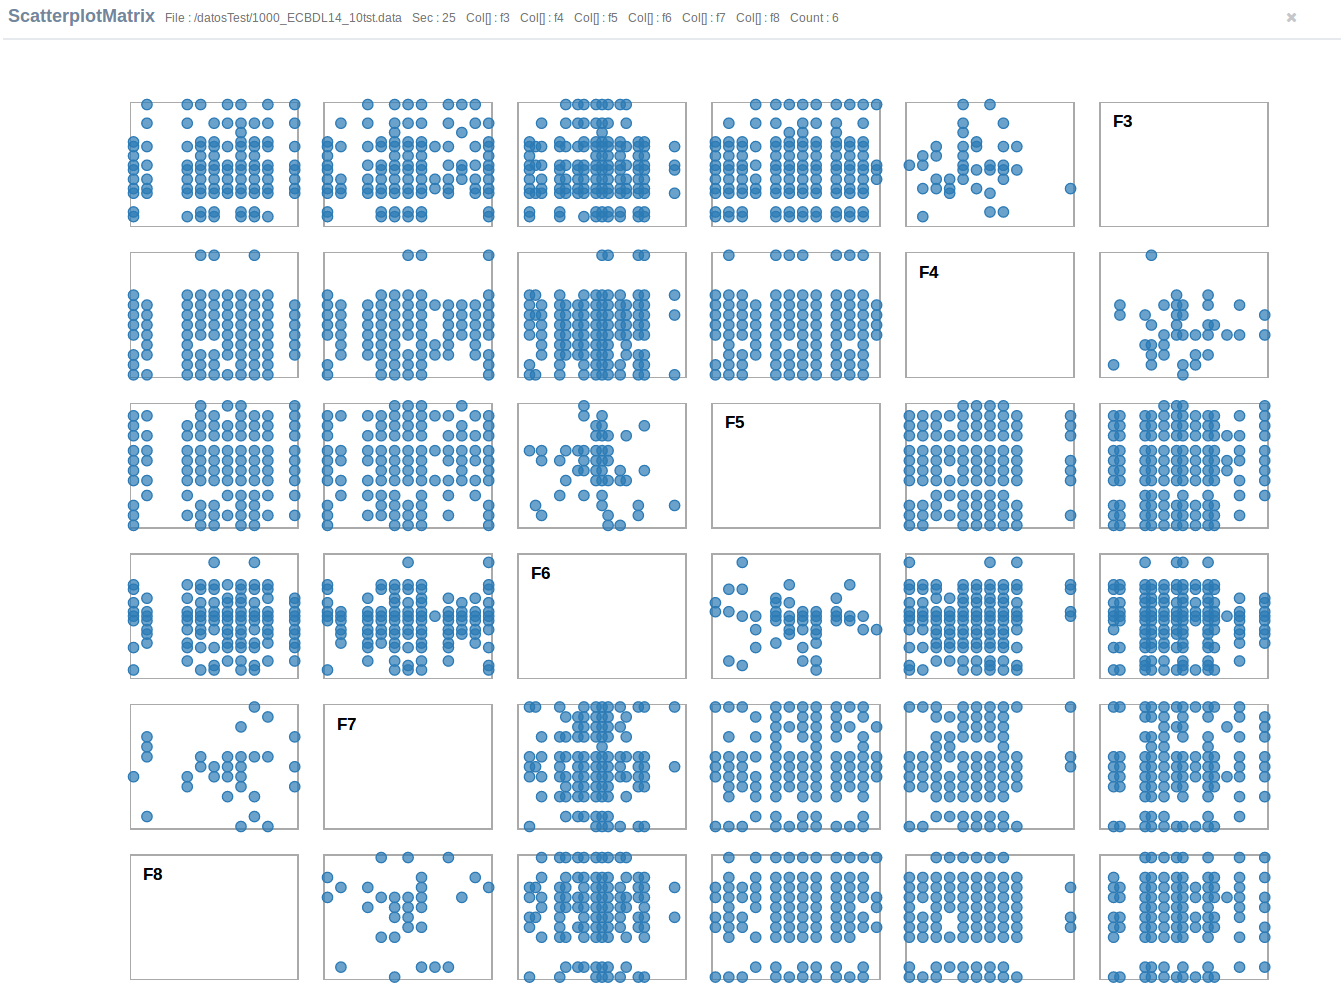
\includegraphics[width=1\linewidth]{imagenes/ejemplo_scatterplotMatrix}
	\caption{Ejemplo de scatterplot matrix}
	\label{fig:ejemploscatterplotmatrix}
\end{figure}

Para la ejecución del scatterplot matrix (ejemplo de URL\footnotemark), los parámetros por orden de inserción son:

\begin{tabular}{|l|l|p{7cm}|}
	\hline 
	\textbf{Campo} & \textbf{Tipo} & \textbf{Descripción} \\ 
	\hline \hline
	\multicolumn{3}{|c|}{\textit{Datos que proporciona la API}} \\
	\hline 
	MongoURL & String & URL del servidor MongoDB activo \\ 
	\hline 
	MongoDB & String & Base de datos dentro de MongoDB \\ 
	\hline 
	MongoCollect& String & Colección dentro de la base de datos en MongoDB \\ 
	\hline \hline
	\multicolumn{3}{|c|}{\textit{Datos que proporciona el usuario}} \\
	\hline 
	File & String & Fichero de entrada de datos, con formato CSV, situado en el HDFS (Hadoop) \\ 
	\hline 
	Sec & Number & Número de secciones sobre los ejes X e Y para la matriz \\ 
	\hline 
	Count & Number & Número de columnas seleccionadas a representar \\ 
	\hline 
	Col & Array[String] & Array con el nombre de las columnas del fichero seleccionadas \\ 
	\hline  
\end{tabular} 

\footnotetext{/scatterplotMatrix?file=\%2FtestData\%2F1000\_ECBDL14\_10tst.csv\&sec=5\&count=2\&col=f3,f4}

\section{Pie Chart}
El diagrama de sectores o Pie Chart, es un gráfico que consiste en dibujar un círculo dividido en sectores, en el que cada uno representa un valor de frecuencia de unos datos. Dicha frecuencia se dibuja aumentando el tamaño del sector dentro del círculo o disminuyéndolo. Por lo general, el gráfico Pie Chart suele representar valores cualitativos.

En la API, el algoritmo utilizado para realizar los cálculos ha sido agrupar los valores cualitativos de una variable seleccionada, de manera que no se repitan, junto con otra variable que represente la frecuencia de los distintos sectores. A cada uno de los valores cualitativos, se le asigna un sector del círculo, y el tamaño lo determina la variable de frecuencia seleccionada. Al igual que ocurre con el gráfico Heatmap, Spark proporciona métodos para agrupar valores en formato 'key-value' con las columnas seleccionadas. Como ha ocurrido en otros gráficos, se puede seleccionar una operación concreta que se desea aplicar sobre la variable de frecuencia. Las operaciones que se pueden seleccionar son de conteo, suma, máximo y mínimo.

Además, se ha añadido una leyenda con el nombre de los valores de los sectores y un color identificativo de cada uno de los sectores. Se puede ver un ejemplo en la figura \ref{fig:ejemplopiechart}
\begin{figure}
	\centering
	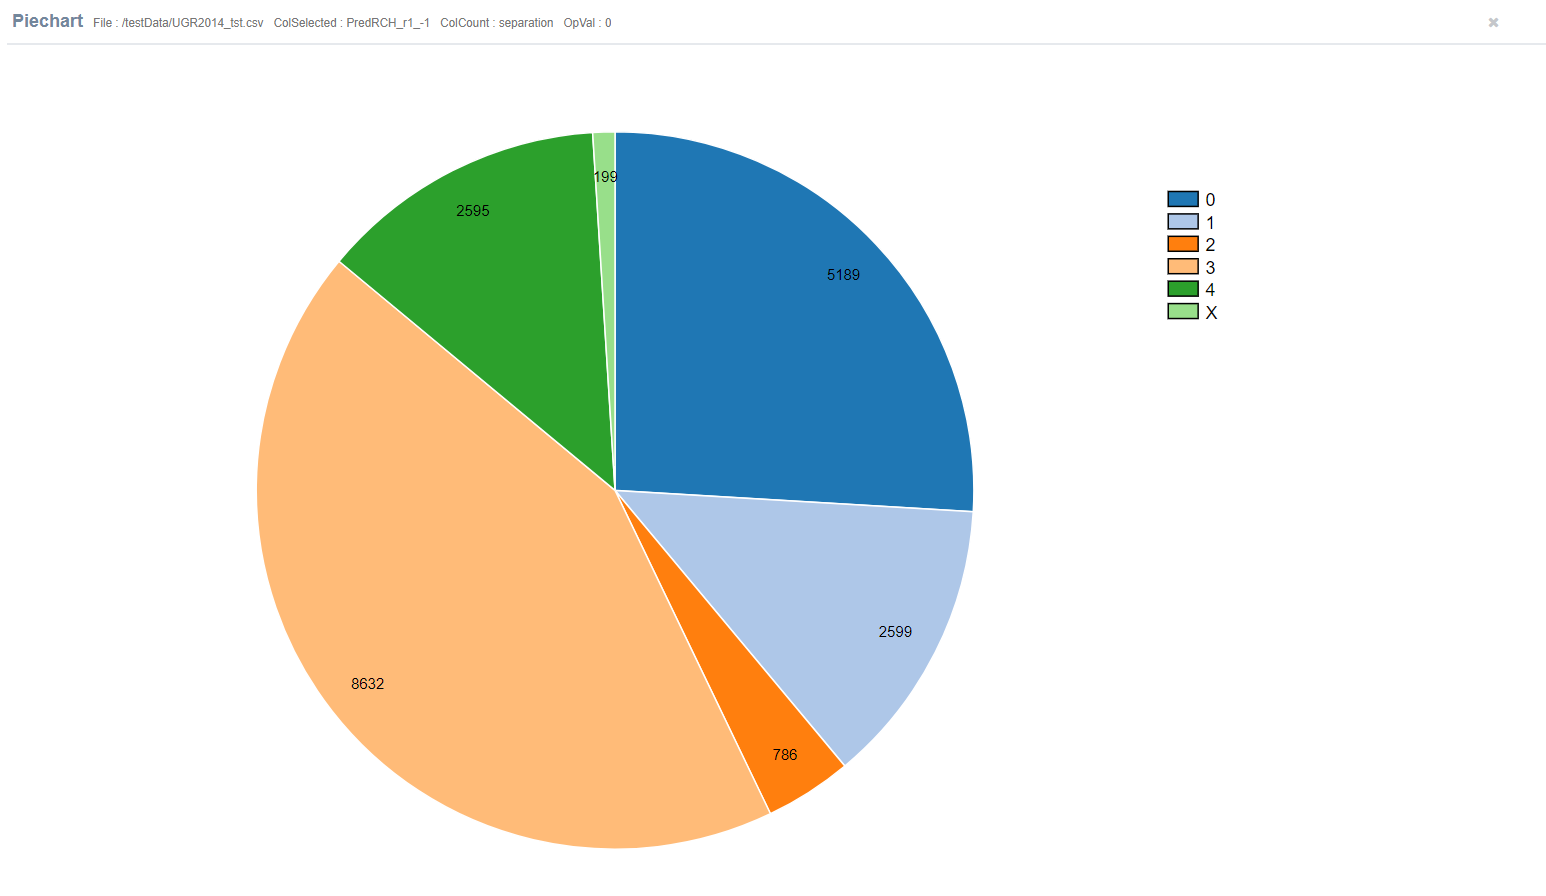
\includegraphics[width=1\linewidth]{imagenes/ejemplo_piechart}
	\caption{Ejemplo de pie chart}
	\label{fig:ejemplopiechart}
\end{figure}

Para la ejecución del pie chart (ejemplo de URL\footnotemark), los parámetros por orden de inserción son:

\begin{tabular}{|l|l|p{7cm}|}
	\hline 
	\textbf{Campo} & \textbf{Tipo} & \textbf{Descripción} \\ 
	\hline \hline
	\multicolumn{3}{|c|}{\textit{Datos que proporciona la API}} \\
	\hline 
	MongoURL & String & URL del servidor MongoDB activo \\ 
	\hline 
	MongoDB & String & Base de datos dentro de MongoDB \\ 
	\hline 
	MongoCollect& String & Colección dentro de la base de datos en MongoDB \\ 
	\hline \hline
	\multicolumn{3}{|c|}{\textit{Datos que proporciona el usuario}} \\
	\hline 
	File & String & Fichero de entrada de datos, con formato CSV, situado en el HDFS (Hadoop) \\ 
	\hline 
	Colselected & String & Columna que representa cada uno de los sectores del círculo \\ 
	\hline 
	Colcount & String & Columna que representa la variable de frecuencia de cada uno de los sectores \\ 
	\hline 
	Opval & Number & Código de la operación para ser aplicada [0-Count, 1-Sum, 2-Max, 3-Min] \\ 
	\hline  
\end{tabular} 

\footnotetext{/piechart?file=\%2FtestData\%2F1000\_ECBDL14\_10tst.csv\&colSelected=f3\&colCount=f4\&opVal=0}

\section{Line Chart}
Los gráficos de líneas representan una serie de puntos conectados por una línea, ajustados a una gran cantidad de datos mediante una sucesión consecutiva de valores, generalmente un periodo continuado de tiempo. Este gráfico es ideal para mostrar tendencias de los datos.

El algoritmo implementado para este gráfico se basa en subdividir los periodos de tiempo o un conjunto de valores que se representa en el eje X, y calcular el número de datos que caen dentro de cada una de las secciones. Es parecido al algoritmo que se utiliza en el Scatterplot solamente que en el LineChart se aplica sobre el eje X, pero no sobre el eje Y del gráfico. Una vez divididos los datos del eje X en sectores y asignados los puntos en cada uno de ellos, basta con calcular el punto medio entre ellos, para obtener un único punto en cada uno de las divisiones. Así, uniendo estos puntos, se obtiene como resultado la línea del gráfico.

Además, la API permite seleccionar un grupo de variables que representen una línea, componiendo así un gráfico de múltiples líneas comparativas, sobre la misma variable de valores continuos asociada al eje X. Se puede ver un ejemplo en la figura \ref{fig:ejemplolinechart}
\begin{figure}
	\centering
	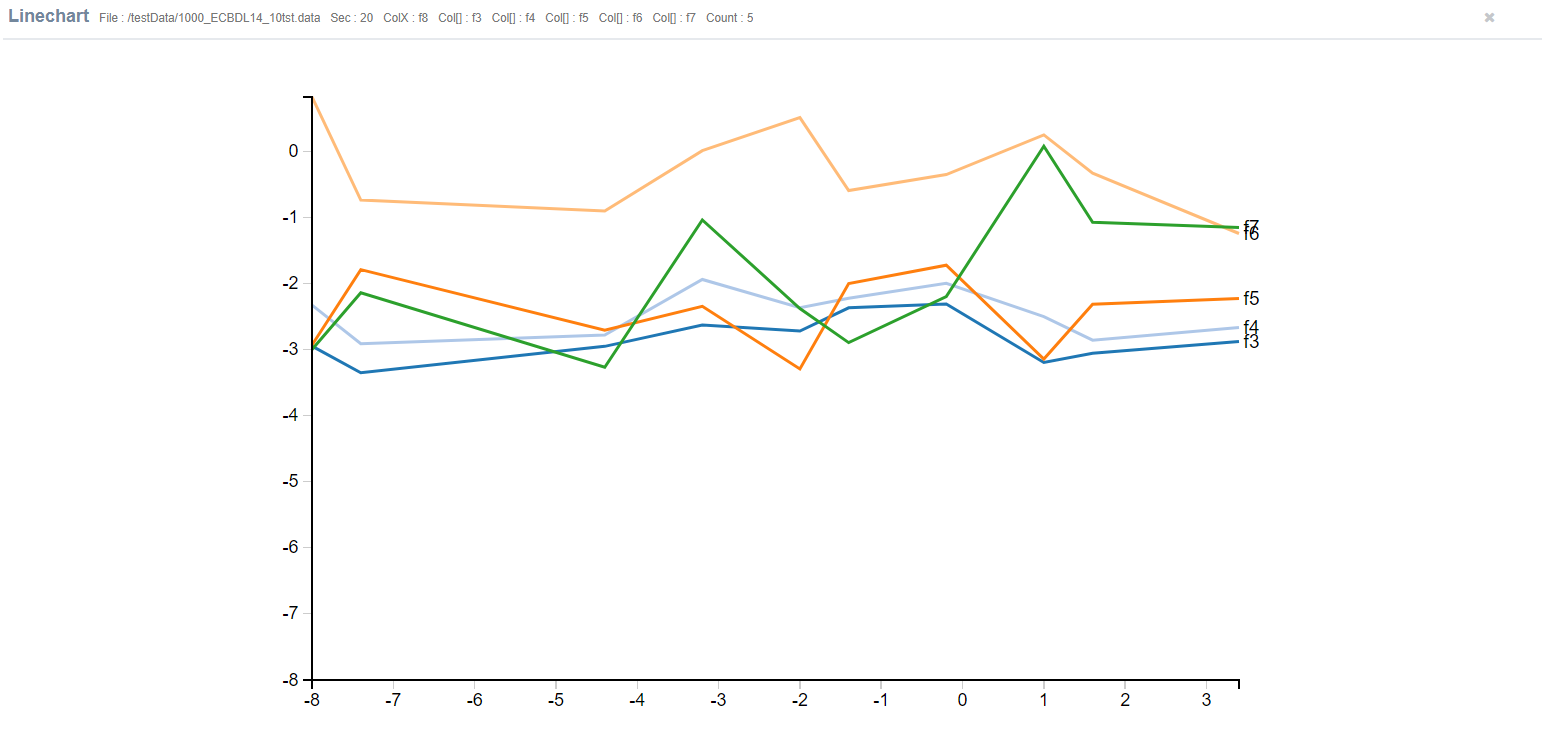
\includegraphics[width=1\linewidth]{imagenes/ejemplo_linechart}
	\caption{Ejemplo de line chart}
	\label{fig:ejemplolinechart}
\end{figure}

Para la ejecución del line chart (ejemplo de URL\footnotemark), los parámetros por orden de inserción son:

\begin{tabular}{|l|l|p{7cm}|}
	\hline 
	\textbf{Campo} & \textbf{Tipo} & \textbf{Descripción} \\ 
	\hline \hline
	\multicolumn{3}{|c|}{\textit{Datos que proporciona la API}} \\
	\hline 
	MongoURL & String & URL del servidor MongoDB activo \\ 
	\hline 
	MongoDB & String & Base de datos dentro de MongoDB \\ 
	\hline 
	MongoCollect& String & Colección dentro de la base de datos en MongoDB \\ 
	\hline \hline
	\multicolumn{3}{|c|}{\textit{Datos que proporciona el usuario}} \\
	\hline 
	File & String & Fichero de entrada de datos, con formato CSV, situado en el HDFS (Hadoop) \\ 
	\hline 
	Sec & Number & Número de secciones que dividir el eje X \\ 
	\hline 
	Colx & String & Columna que represente los valores continuos del eje X \\ 
	\hline 
	Count & Number & Número de columnas seleccionadas a representar por líneas \\ 
	\hline  
	Col & Array[String] & Array con el nombre de las columnas del fichero seleccionadas \\ 
	\hline
\end{tabular} 

\footnotetext{/linechart?file=\%2FtestData\%2F1000\_ECBDL14\_10tst.csv\&sec=10\&colX=f3\&count=2\&col=f4,f5}

\section{Stacked Area Chart}
El gráfico Stacked Area Chart utiliza una serie de variables con múltiples datos. Cada una de ellas comienza a partir de último punto sobre el eje X de la variable anterior. El gráfico representa todos los trazos de cada una de las variables acumuladas una sobre la otra. El Stacked Area Chart muestra las relaciones entre las distintas variables seleccionadas, ayudando a visualizar como contribuyen cada una al total acumulado.

El algoritmo para obtener los datos necesarios para pintarlo es el mismo que el aplicado en el Line chart. La diferencia está en la manera de visualizarlos, aportando otro tipo de información al usuario. Se puede ver un ejemplo en la figura \ref{fig:ejemplostackedareachart}

\begin{figure}
	\centering
	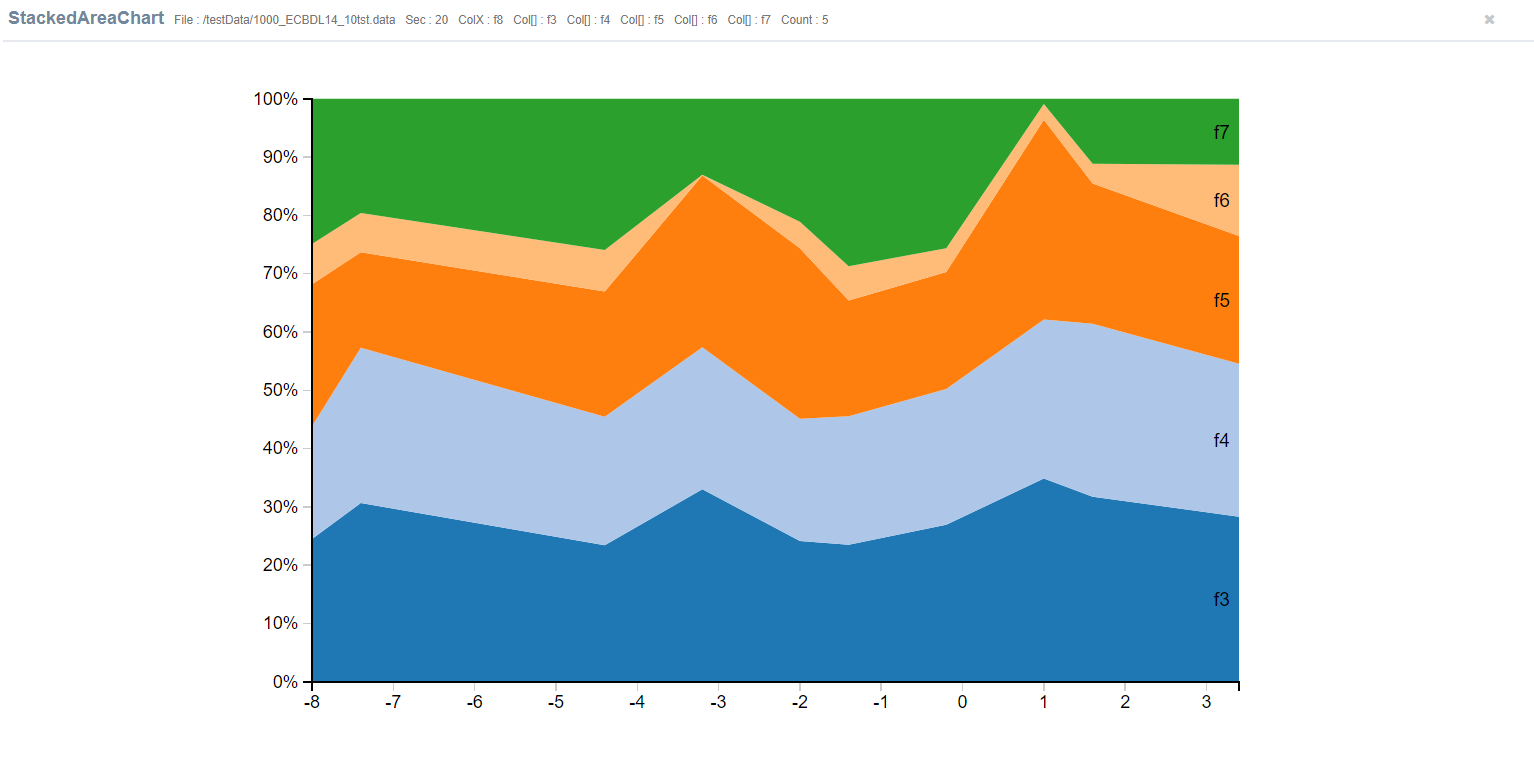
\includegraphics[width=1\linewidth]{imagenes/ejemplo_stackedareachart}
	\caption{Ejemplo de un stacked area chart}
	\label{fig:ejemplostackedareachart}
\end{figure}

Para la ejecución del stacked area chart (ejemplo de URL\footnotemark), los parámetros por orden de inserción son:

\begin{tabular}{|l|l|p{7cm}|}
	\hline 
	\textbf{Campo} & \textbf{Tipo} & \textbf{Descripción} \\ 
	\hline \hline
	\multicolumn{3}{|c|}{\textit{Datos que proporciona la API}} \\
	\hline 
	MongoURL & String & URL del servidor MongoDB activo \\ 
	\hline 
	MongoDB & String & Base de datos dentro de MongoDB \\ 
	\hline 
	MongoCollect& String & Colección dentro de la base de datos en MongoDB \\ 
	\hline \hline
	\multicolumn{3}{|c|}{\textit{Datos que proporciona el usuario}} \\
	\hline 
	File & String & Fichero de entrada de datos, con formato CSV, situado en el HDFS (Hadoop) \\ 
	\hline 
	Sec & Number & Número de secciones que dividir el eje X \\ 
	\hline 
	Colx & String & Columna que represente los valores continuos del eje X \\ 
	\hline 
	Count & Number & Número de columnas seleccionadas a representar por líneas \\ 
	\hline  
	Col & Array[String] & Array con el nombre de las columnas del fichero seleccionadas \\ 
	\hline
\end{tabular} 

\footnotetext{/stackedAreaChart?file=\%2FtestData\%2F1000\_ECBDL14\_10tst.csv\&sec=10\&colX=f3\&count=2\&col=f4,f5}

\section{Bar Chart}
Un gráfico Bar Chart resume un grupo de variables de tipo cuantitativas, usando otra variable que represente un valor numérico. Gráficamente, este valor representa la altura de cada una de las barras, teniendo información visual sobre la comparativa entre las distintas variables cuantitativas de cada una de las barras. Probablemente sea el gráfico más sencillo, pero a su vez el que más información aporta sobre el comportamiento de los datos subyacentes. 

Para el Bar Chart, se ha utilizado el mismo algoritmo que se ha implementado para el Pie Chart. Utiliza una variable o columna que representa cada uno de los valores del eje Y, agrupados para evitar repetición, sobre otra columna numérica a la que se le aplica una de las operaciones disponibles, las mismas que se pueden aplicar sobre el Pie Chart. Destacar que el gráfico se representa de manera horizontal, para representar en barras un mayor número de variables. Se puede ver un ejemplo en la figura \ref{fig:ejemplobarchart}
\begin{figure}
	\centering
	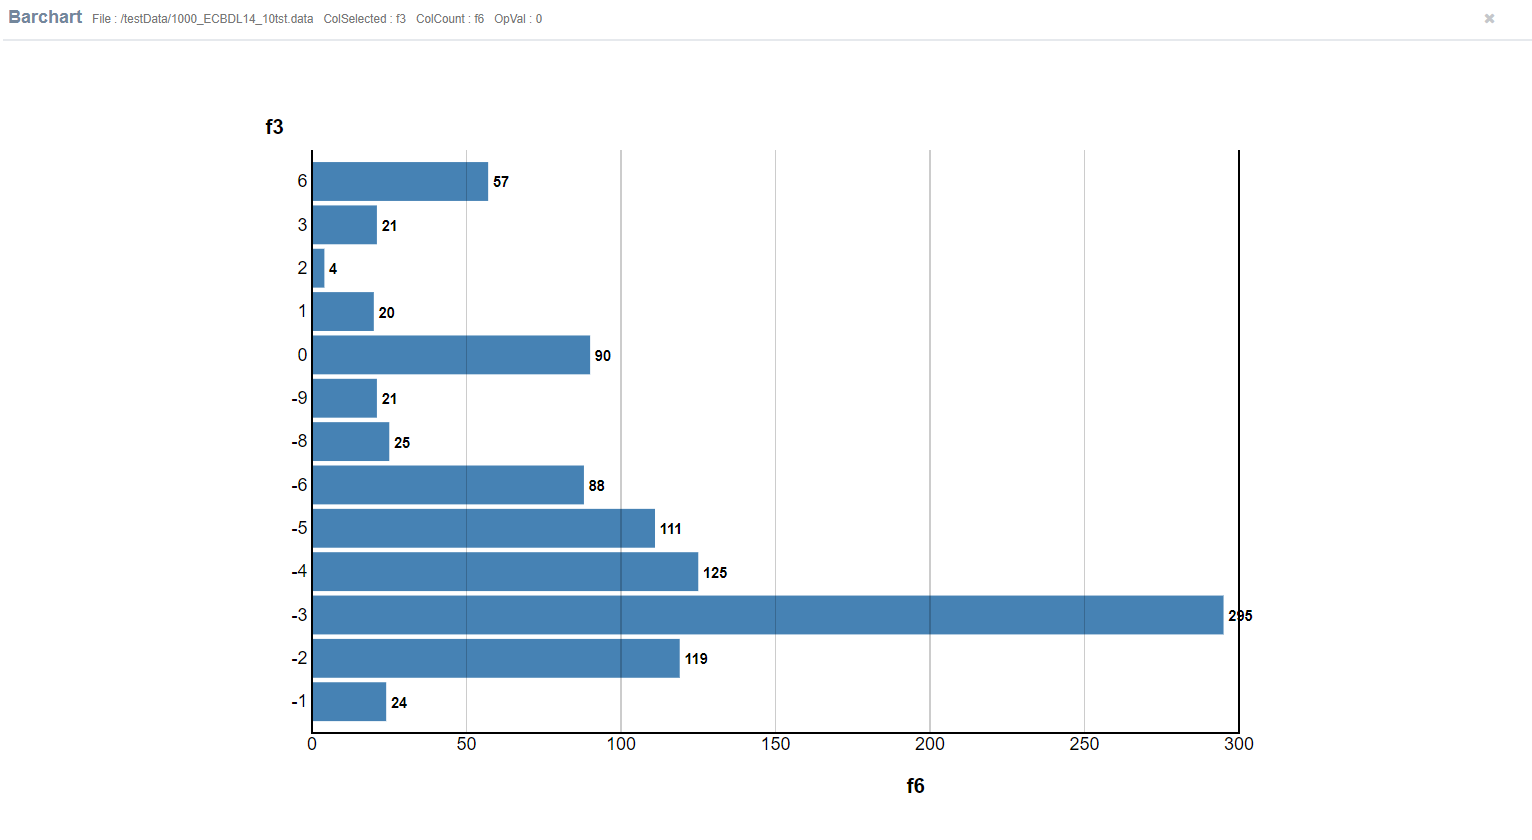
\includegraphics[width=1\linewidth]{imagenes/ejemplo_barchart}
	\caption{Ejemplo de bar chart}
	\label{fig:ejemplobarchart}
\end{figure}

Para la ejecución del bar chart (ejemplo de URL\footnotemark), los parámetros por orden de inserción son:

\begin{tabular}{|l|l|p{7cm}|}
	\hline 
	\textbf{Campo} & \textbf{Tipo} & \textbf{Descripción} \\ 
	\hline \hline
	\multicolumn{3}{|c|}{\textit{Datos que proporciona la API}} \\
	\hline 
	MongoURL & String & URL del servidor MongoDB activo \\ 
	\hline 
	MongoDB & String & Base de datos dentro de MongoDB \\ 
	\hline 
	MongoCollect& String & Colección dentro de la base de datos en MongoDB \\ 
	\hline \hline
	\multicolumn{3}{|c|}{\textit{Datos que proporciona el usuario}} \\
	\hline 
	File & String & Fichero de entrada de datos, con formato CSV, situado en el HDFS (Hadoop) \\ 
	\hline 
	Colselected & String & Columna que representa cada uno de las barras del diagrama \\ 
	\hline 
	Colcount & String & Columna que representa la variable de frecuencia de cada uno de las barras \\ 
	\hline 
	Opval & Number & Código de la operación para ser aplicada [0-Count, 1-Sum, 2-Max, 3-Min] \\ 
	\hline  
\end{tabular} 

\footnotetext{/barchart?file=\%2FtestData\%2F1000\_ECBDL14\_10tst.csv\&colSelected=f3\&colCount=f4\&opVal=0}
\chapter{Conclusiones}

La creación de herramientas capaces de analizar y presentar de manera gráfica grandes cantidades de datos es una de las necesidades que demanda actualmente el mercado de la tecnología. Teniendo esto en mente, el objetivo principal del proyecto se han cumplido.

La creación de una biblioteca capaz de generar representaciones gráficas de un conjunto de datos de tipo 'Big Data', se ha cumplido con éxito. Obtener los valores necesarios para generar un gráfico a partir de este tipo de datos, apoyándose en herramientas específicas para Big Data, ha sido la clave para que este proyecto funcione. La parte difícil ha sido comunicar entre si estas herramientas para funcionar como una sola, pero todos los problemas se han superado. Tener la posibilidad de utilizar más fuentes de datos, no solo de tipo CSV, sino también JSON o incluso bases de datos SQL, no formaban parte de los objetivos, pero sí se planteó como una futura mejora.

También se ha logrado el objetivo de implementar una API RESTful. Esta permite acceder a cada una de los métodos diseñados en el sistema de manera individual para obtener información sobre ello y probar su funcionamiento.

Por último, el diseño de una interfaz web para utilizar todas las funciones implementadas en el sistema, también se ha cumplido como objetivo. Se trata de una interfaz sencilla, con la accesibilidad que proporciona una web y con la eficacia de poder gestionar las funciones de manera asíncrona. Además está diseñada bajo una estructura bien jerarquizada, de manera que se pueda modificar cualquier elemento o añadir nuevos fácilmente.

Uno de los aspectos que han faltado por implementar, también por falta de tiempo, ha sido tener una gestión de usuarios de acceso al sistema e implementar un apartado de configuración de las variables del sistema, de manera que el usuario no tenga necesidad de introducirse en el código de la aplicación. 

Poder desarrollar esta aplicación supone un avance en el campo del Big Data en cuanto a la posibilidad de entender, de una manera gráfica, qué ocurre con los datos en tiempo real. Esto significa que para medianas y grandes organizaciones que generan cada día una multitud de datos, tan variados y de distintas procedencias, este tipo de aplicaciones se vuelven imprescindibles para poder tomar las las mejores decisiones. 

\appendix
\chapter{Listado de Funciones de la API}
En este apéndice se va a listar cada una de los métodos implementadas en el sistema, con una breve descripción de su funcionamiento, ordenadas alfabéticamente:

\begin{tabular}{|l|p{8cm}|}
	\hline 
	\textbf{Función} & \textbf{Descripción} \\ 
	\hline 
	About & Devuelve información sobre la aplicación y sus desarrolladores \\ 
	\hline 
	Api-docs & Genera una nueva ventana con la documentación generada por Swagger \\ 
	\hline 
	Barchart & Devuelve los datos necesarios para dibujar un diagrama de barras \\ 
	\hline 
	Boxplot & Devuelve los datos necesarios para dibujar un diagrama de cajas \\ 
	\hline 
	Bubblechart & Devuelve los datos necesarios para dibujar un diagrama de burbujas \\ 
	\hline 
	Files & Devuelve una lista con los archivos del HDFS en la ruta especificada  \\ 
	\hline 
	Heatmap & Devuelve los datos necesarios para dibujar un mapa de calor \\ 
	\hline 
	Histogram & Devuelve los datos necesarios para dibujar un histograma \\ 
	\hline 
	Linechart & Devuelve los datos necesarios para dibujar un diagrama de líneas \\ 
	\hline 
	Piechart & Devuelve los datos necesarios para dibujar un diagrama de sectores \\ 
	\hline 
	Scatterplot & Devuelve los datos necesarios para dibujar un diagrama de puntos \\ 
	\hline 
	ScatterplotMatrix & Devuelve los datos necesarios para dibujar una matriz de diagramas de puntos \\ 
	\hline 
	StackedAreaChart & Devuelve los datos necesarios para dibujar un diagrama de áreas \\ 
	\hline 
	Summary & Devuelve información sobre el archivo seleccionado del HDFS \\ 
	\hline 
\end{tabular} 

\listoffigures

\backmatter
% bibliography, glossary and index would go here.

%\bibliographystyle{jtbnew}
\bibliographystyle{unsrt}
\bibliography{./bibliografia/bibliografia}

\end{document}